% !Mode:: "TeX:UTF-8"
% !TEX root = ..\thesis.tex
\chapter{实验结果图表}
%模型1 和模型2 运用其相应的不同算法得到了目标函数值、流水线均衡率等结果。
%不同决策参数$\lambda_1$、流水线数量$m$及订单数量$n$的环境下,模型1 的所得结果如\reff{fig:result1} -- \reff{fig:result3}所示,模型2 的所得结果如\reff{fig:result4} -- \reff{fig:result9}所示。
\vspace{-1em}
% !Mode:: "TeX:UTF-8"
% !TEX root = ..\thesis.tex
\begin{table}[h]
  \centering
  \caption{Cyc -- ATC、Cyc -- Tabu、Vtr -- Tabu 算法求解模型1 目标函数值($\lambda_1 = 0.4$)}
  \subfloat{  \begin{tabular}{cccccccc}
    \toprule
    流水线数量($m$) & 订单数量($n$) &$ 20    $&$ 30    $&$ 50    $&$ 70    $&$ 100   $&$ 150 $\\
    \midrule
    \multirow{3}[0]{*}{$5$} & Cyc - ATC &$ 5581  $&$ 11585 $&$ 35912 $&$ 58236 $&$ 116557 $&$ 289619$ \\
          & Cyc - Tabu &$ 4945  $&$ 9627  $&$ 29568.6 $&$ 46551.6 $&$ 94332.8 $&$ 229521.2$ \\
          & Vtr - Tabu &$ 4203  $&$ 8003.4 $&$ 25104.8 $&$ 39186.6 $&$ 79288.2 $&$ 187143.2$ \\
    \multirow{3}[0]{*}{$6$} & Cyc - ATC &$ 4756  $&$ 9840.6 $&$ 30910 $&$ 52190.8 $&$ 105418.6 $&$ 262350.8$ \\
          & Cyc - Tabu &$ 4117  $&$ 8133.8 $&$ 25205 $&$ 40733.8 $&$ 81944 $&$ 205849$ \\
          & Vtr - Tabu &$ 3602  $&$ 6980.4 $&$ 20784.6 $&$ 34011.2 $&$ 68408.6 $&$ 167215$ \\
    \multirow{3}[0]{*}{$7$} & Cyc - ATC &$ 4661  $&$ 9583.6 $&$ 30563.2 $&$ 51475.8 $&$ 104903.8 $&$ 260983.4$ \\
          & Cyc - Tabu &$ 3979  $&$ 7978.8 $&$ 24748.6 $&$ 40596.8 $&$ 81936.6 $&$ 204826.8$ \\
          & Vtr - Tabu &$ 3484  $&$ 6828.2 $&$ 20403.2 $&$ 33730.6 $&$ 67947.2 $&$ 166778$ \\
    \bottomrule
    \end{tabular}
}\\
\subfloat{
\begin{tabular}{ccccccc}
\toprule
流水线数量($m$) & 订单数量($n$) &$ 200   $&$ 300   $&$ 500   $&$ 750   $&$ 1000$ \\
\midrule
\multirow{3}[0]{*}{$5$} & Cyc - ATC &$ 551295 $&$ 1229710 $&$ 3357427 $&$ 7388241 $&$ 13365000$ \\
      & Cyc - Tabu &$ 442831.2 $&$ 983565 $&$ 2692518.6 $&$ 5863540 $&$ 10587368$ \\
      & Vtr - Tabu &$ 369743.2 $&$ 813236.6 $&$ 2218180.4 $&$ 4809759.4 $&$ 8702396.2$ \\
\multirow{3}[0]{*}{$6$} & Cyc - ATC &$ 491435.6 $&$ 1105733 $&$ 3067669.6 $&$ 6878062.6 $&$ 12701013$ \\
      & Cyc - Tabu &$ 442831.2 $&$ 876495 $&$ 2403561.6 $&$ 5411006 $&$ 9985752$ \\
      & Vtr - Tabu &$ 369743.2 $&$ 716757 $&$ 1960913.2 $&$ 4370667.2 $&$ 8191029.4$ \\
\multirow{3}[0]{*}{$7$} & Cyc - ATC &$ 491485.4 $&$ 1098758.2 $&$ 3064412.4 $&$ 6886176.4 $&$ 12758606$ \\
      & Cyc - Tabu &$ 392325.4 $&$ 872953.2 $&$ 2411157.6 $&$ 5400248 $&$ 9988071.2$ \\
      & Vtr - Tabu &$ 322642.8 $&$ 714846 $&$ 1957291 $&$ 4340928.4 $&$ 8131055.6$ \\
\bottomrule
\end{tabular}
}
\label{tab:resultmodel104}
\end{table}
% !Mode:: "TeX:UTF-8"
% !TEX root = ..\thesis.tex
\begin{table}[!h]
\centering
\caption{Cyc -- ATC、Cyc -- Tabu、Vtr -- Tabu 算法求解模型1 目标函数值($\lambda_1 = 0.5$)}
\subfloat{
\begin{tabular}{cccccccc}
\toprule
流水线数量($m$) & 订单数量($n$) &$ 20    $&$ 30    $&$ 50    $&$ 70    $&$ 100   $&$ 150$ \\
\midrule
\multirow{3}[0]{*}{$5$} & Cyc - ATC &$ 4780  $&$ 9978  $&$ 31425 $&$ 51791 $&$ 103325 $&$ 264838$ \\
      & Cyc - Tabu &$ 4199  $&$ 8192  $&$ 25250 $&$ 40170 $&$ 81942 $&$ 205510$ \\
      & Vtr - Tabu &$ 3541  $&$ 6758.5 $&$ 21498 $&$ 33480 $&$ 67960.5 $&$ 164038.5$ \\
\multirow{3}[0]{*}{$6$} & Cyc - ATC &$ 4118  $&$ 8740  $&$ 27933.5 $&$ 47573.5 $&$ 96258 $&$ 248084.5$ \\
      & Cyc - Tabu &$ 3515  $&$ 7129.5 $&$ 22146 $&$ 36511 $&$ 73294.5 $&$ 190964$ \\
      & Vtr - Tabu &$ 3050  $&$ 6011.5 $&$ 17978.5 $&$ 29580.5 $&$ 59568.5 $&$ 151768.5$ \\
\multirow{3}[0]{*}{$7$} & Cyc - ATC &$ 3995  $&$ 8527  $&$ 27745.5 $&$ 46939 $&$ 95269.5 $&$ 247589.5$ \\
      & Cyc - Tabu &$ 3416  $&$ 6986.5 $&$ 21855.5 $&$ 36205.5 $&$ 73165 $&$ 190116$ \\
      & Vtr - Tabu &$ 2985  $&$ 5888.5 $&$ 17547.5 $&$ 29350.5 $&$ 59311 $&$ 151254.5$ \\
\bottomrule
\end{tabular}
}\\
\subfloat{
\begin{tabular}{ccccccc}
\toprule
流水线数量($m$) & 订单数量($n$) &$ 200   $&$ 300   $&$ 500   $&$ 750   $&$ 1000$ \\
\midrule
\multirow{3}[0]{*}{$5$} & Cyc - ATC &$ 495784 $&$ 1100705 $&$ 3026502 $&$ 6693485 $&$ 12058054$ \\
      & Cyc - Tabu &$ 389869.5 $&$ 863417.5 $&$ 2377471 $&$ 5200593 $&$ 9344528$ \\
      & Vtr - Tabu &$ 319789 $&$ 700956.5 $&$ 1922185 $&$ 4178898.5 $&$ 7527673.5$ \\
\multirow{3}[0]{*}{$6$} & Cyc - ATC &$ 461957.5 $&$ 1031038 $&$ 2896712.5 $&$ 6436879.5 $&$ 11697210$ \\
      & Cyc - Tabu &$ 389869.5 $&$ 799935 $&$ 2237562 $&$ 4992762.5 $&$ 9032005$ \\
      & Vtr - Tabu &$ 319789 $&$ 653621.5 $&$ 1779688 $&$ 3977370 $&$ 7304717.5$ \\
\multirow{3}[0]{*}{$7$} & Cyc - ATC &$ 459643.5 $&$ 1030355.5 $&$ 2888723.5 $&$ 6402199.5 $&$ 11663579$ \\
      & Cyc - Tabu &$ 359077 $&$ 796370 $&$ 2230433 $&$ 4974146 $&$ 9026475.5$ \\
      & Vtr - Tabu &$ 291215 $&$ 647937.5 $&$ 1772640 $&$ 3959083.5 $&$ 7289415$ \\
\bottomrule
\end{tabular}
}
\label{tab:resultmodel105}
\end{table}
\begin{sidewaysfigure}
\centering
\subfloat[$n = 20$]{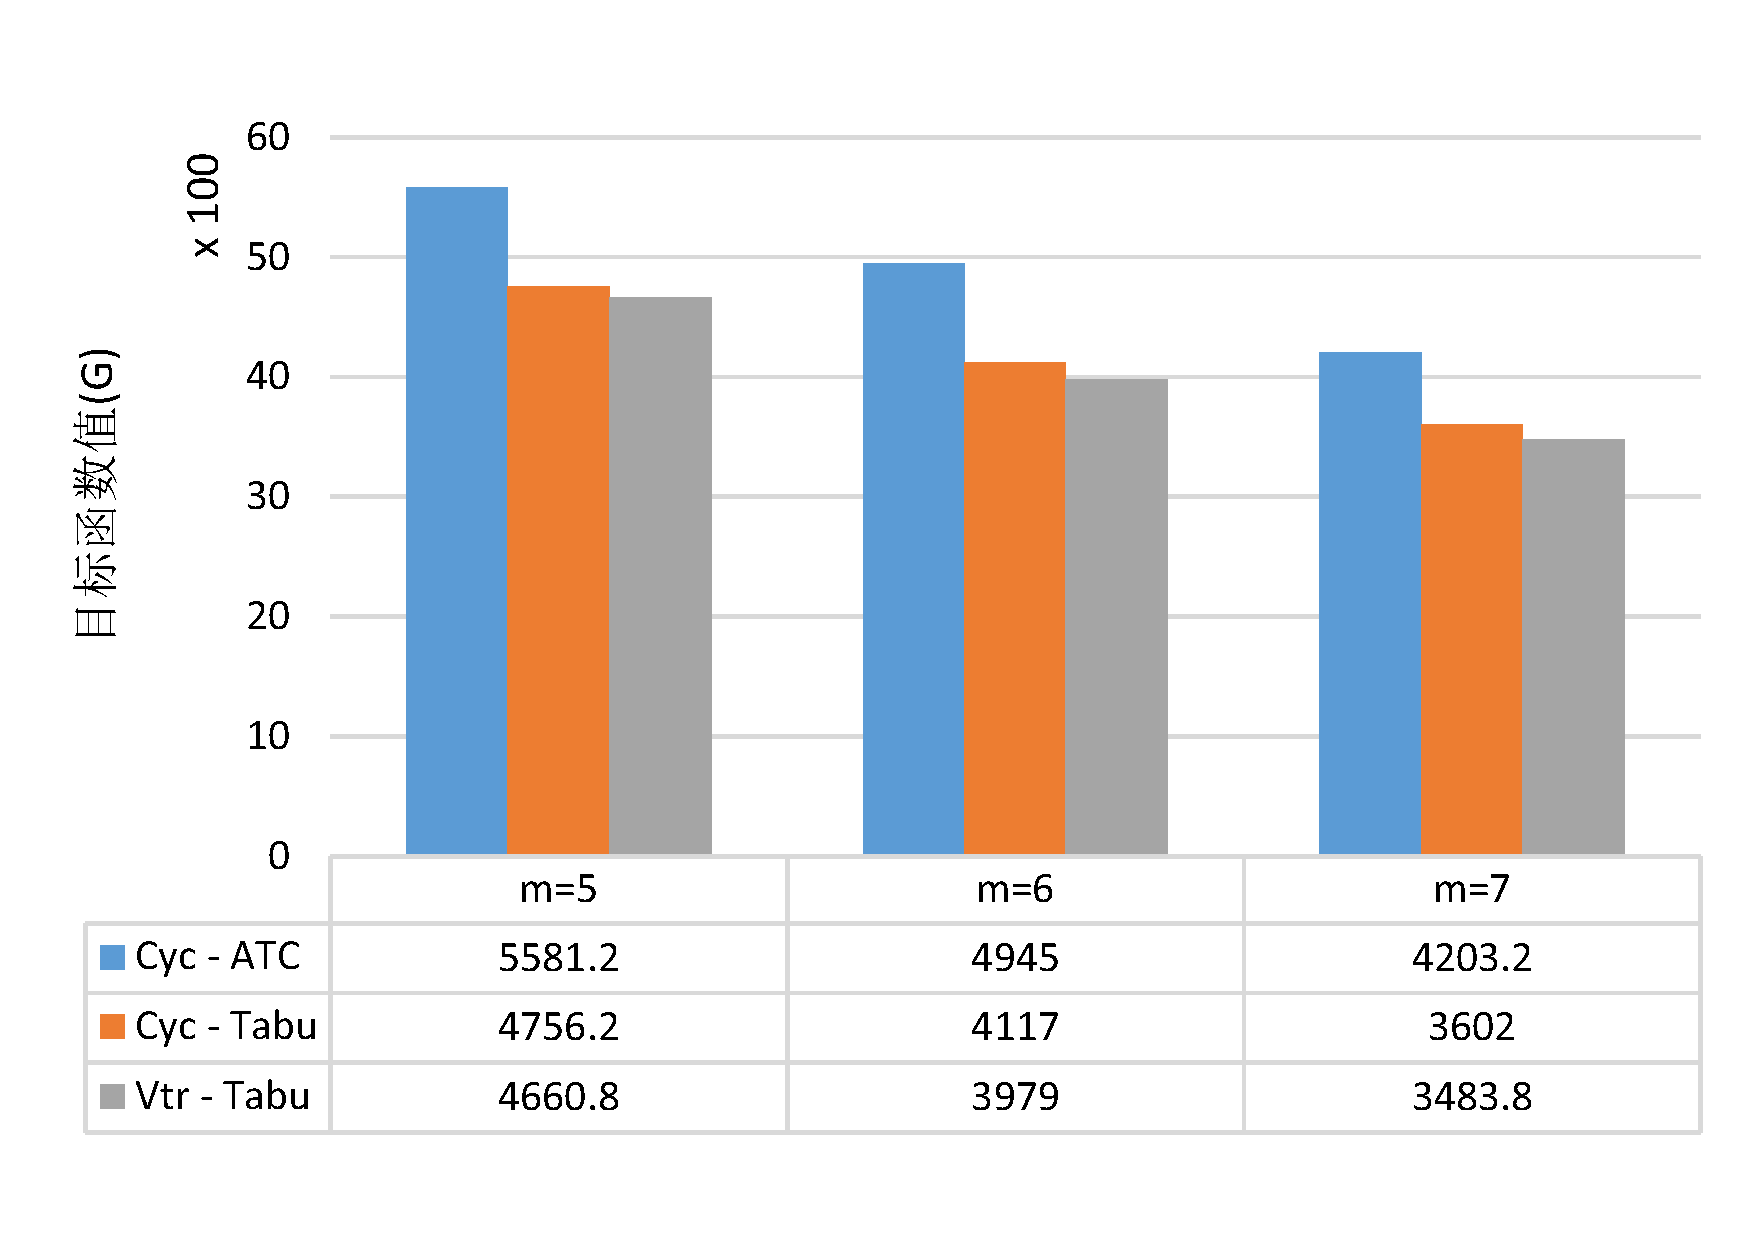
\includegraphics[height = 6cm, angle = -90]{basic_04_20}}
\subfloat[$n = 30$]{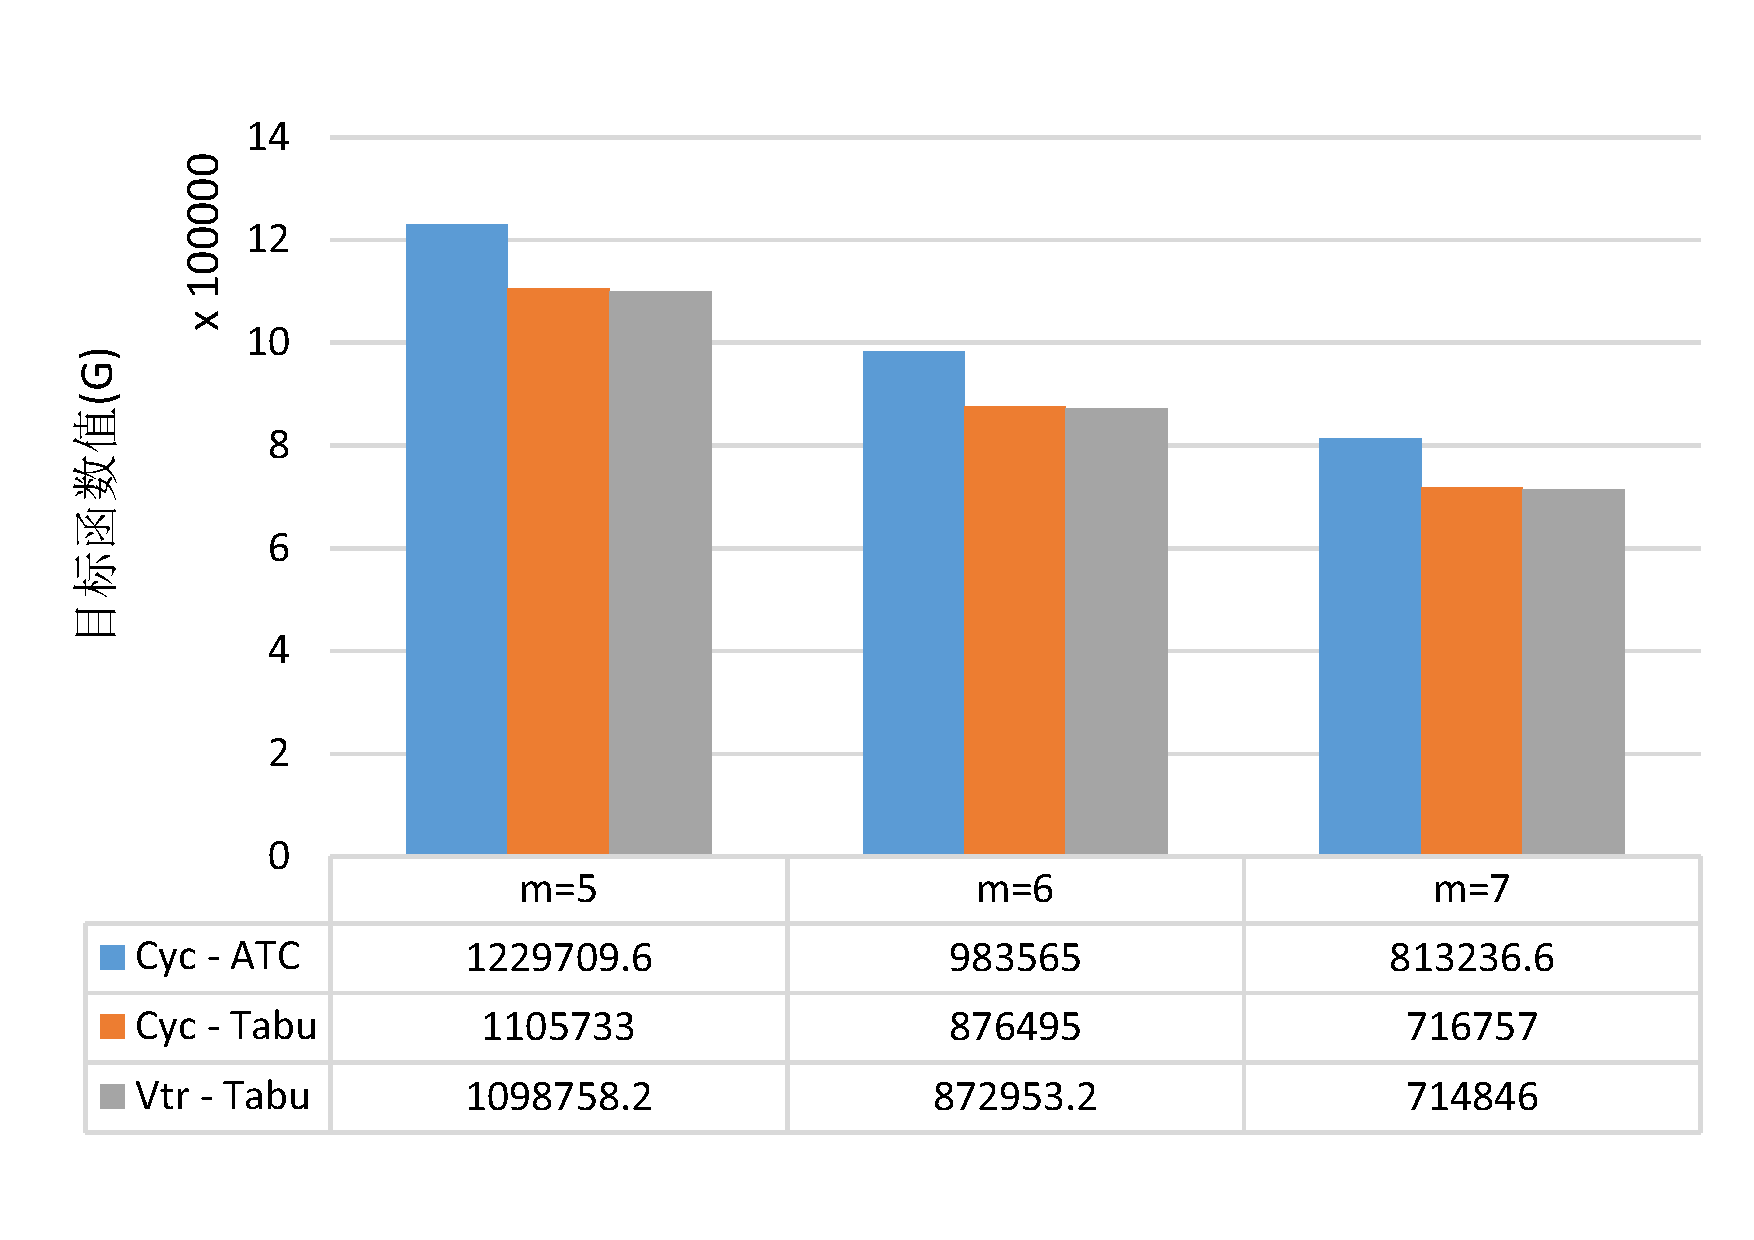
\includegraphics[height = 6cm, angle = -90]{basic_04_300}}
\subfloat[$n = 50$]{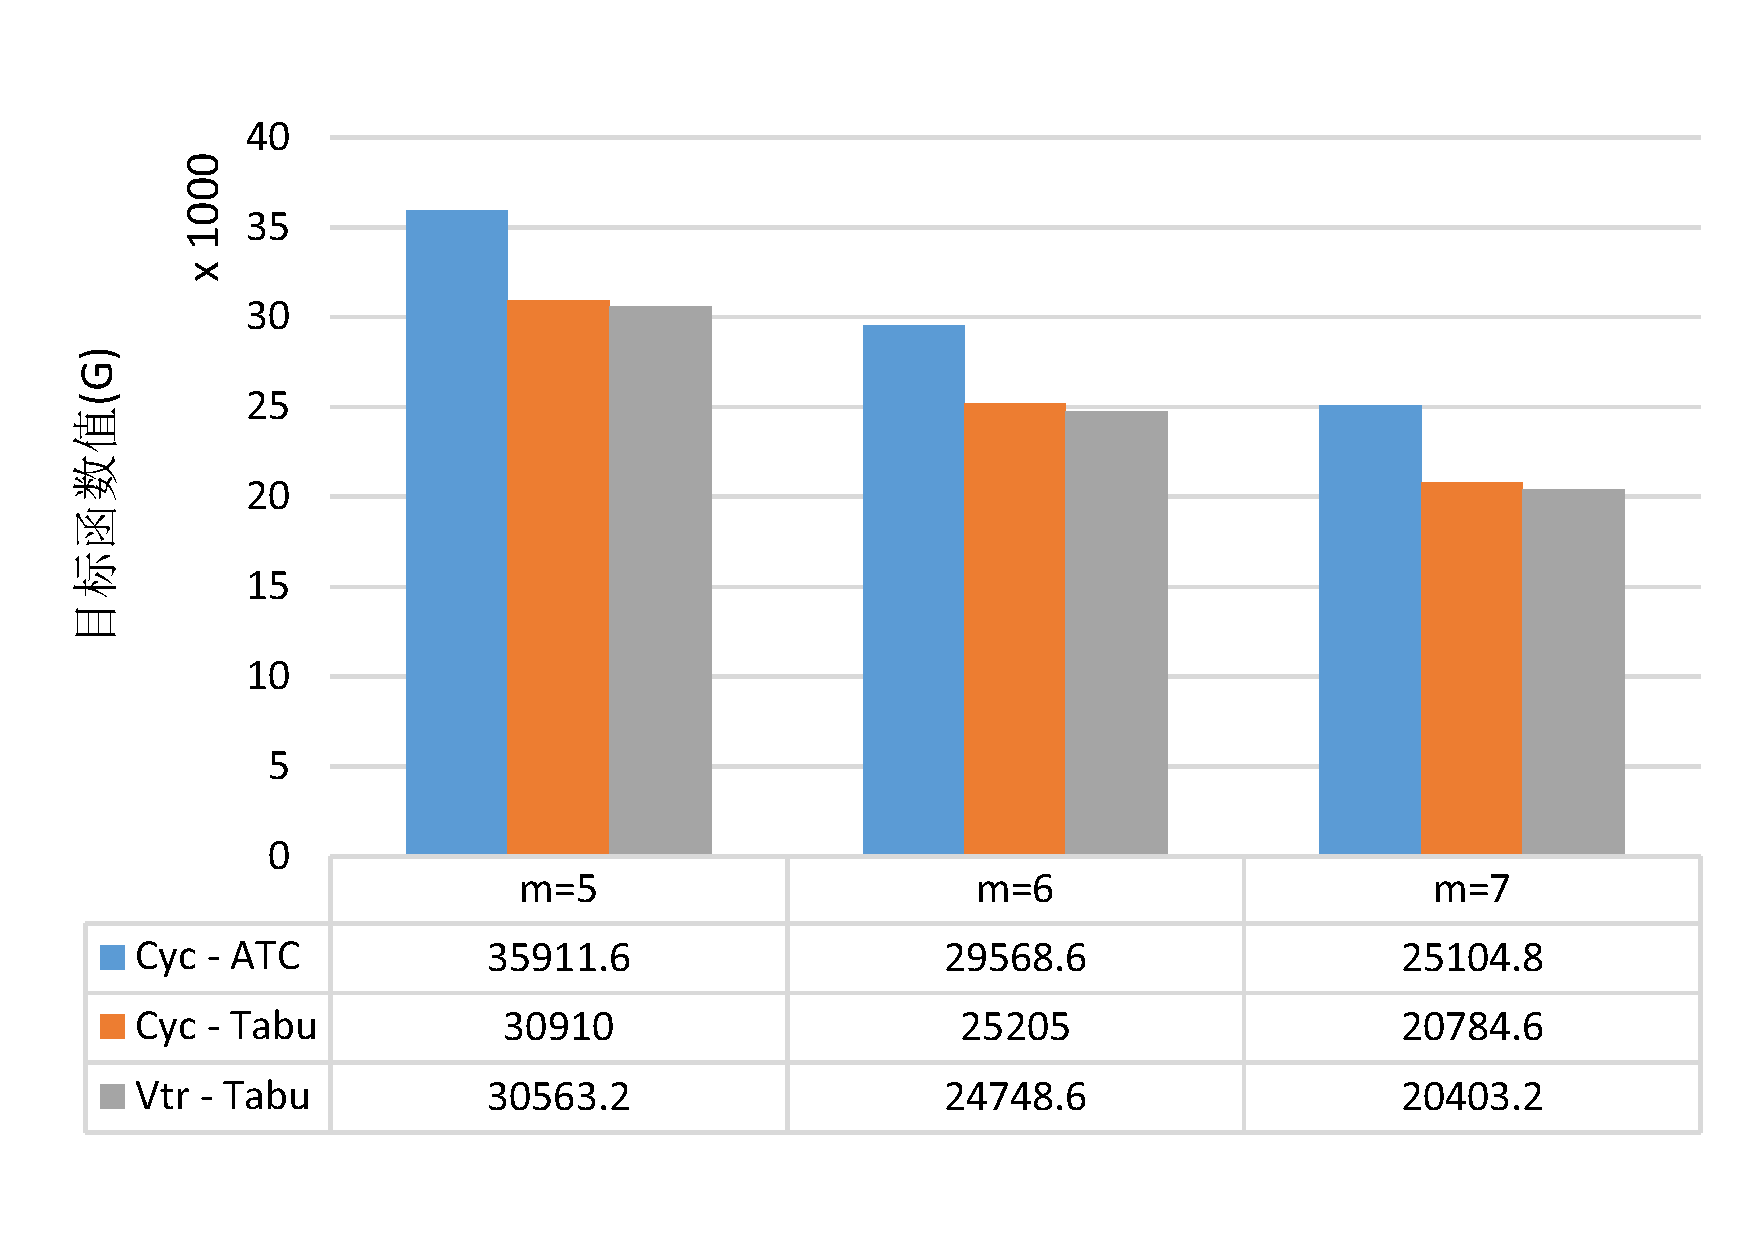
\includegraphics[height = 6cm, angle = -90]{basic_04_50}}
\subfloat[$n = 70$]{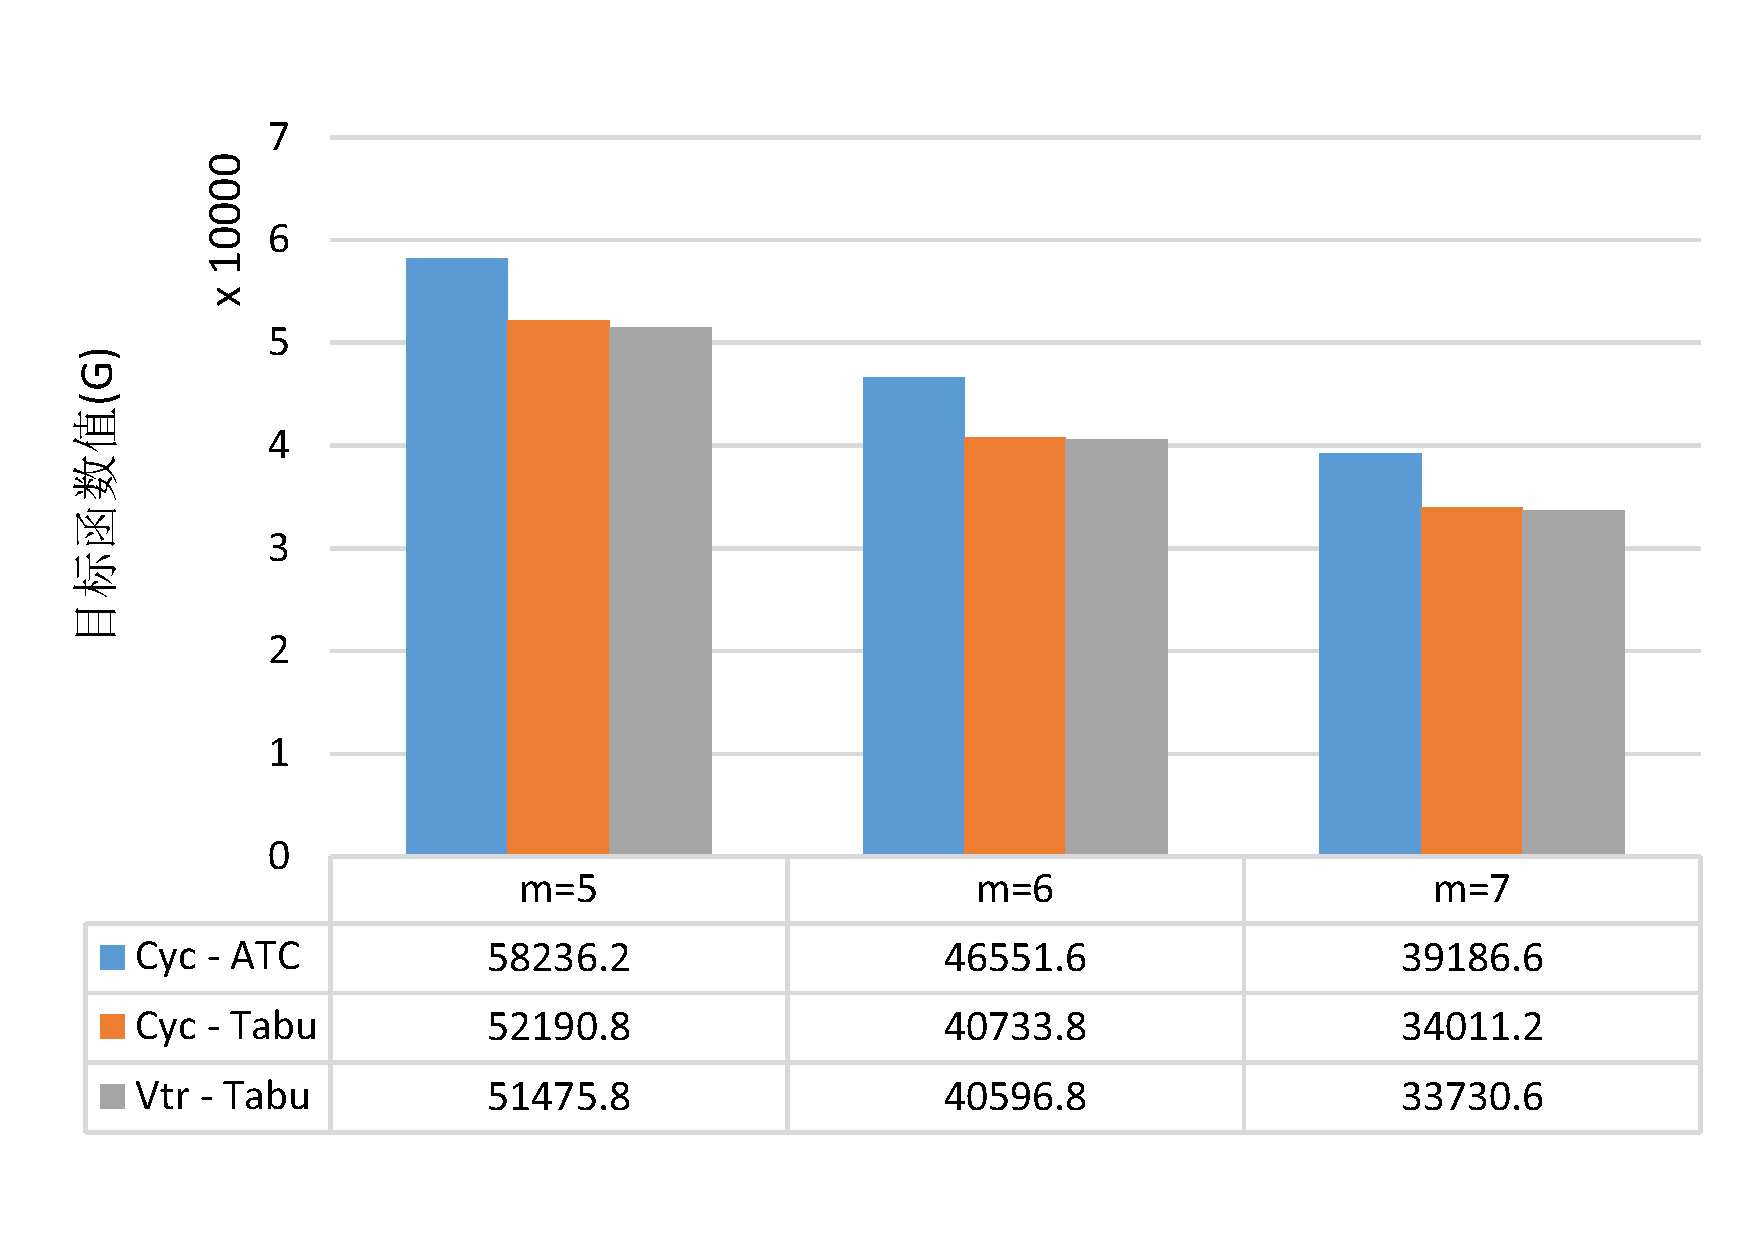
\includegraphics[height = 6cm, angle = -90]{basic_04_70}}\\
\subfloat[$n = 100$]{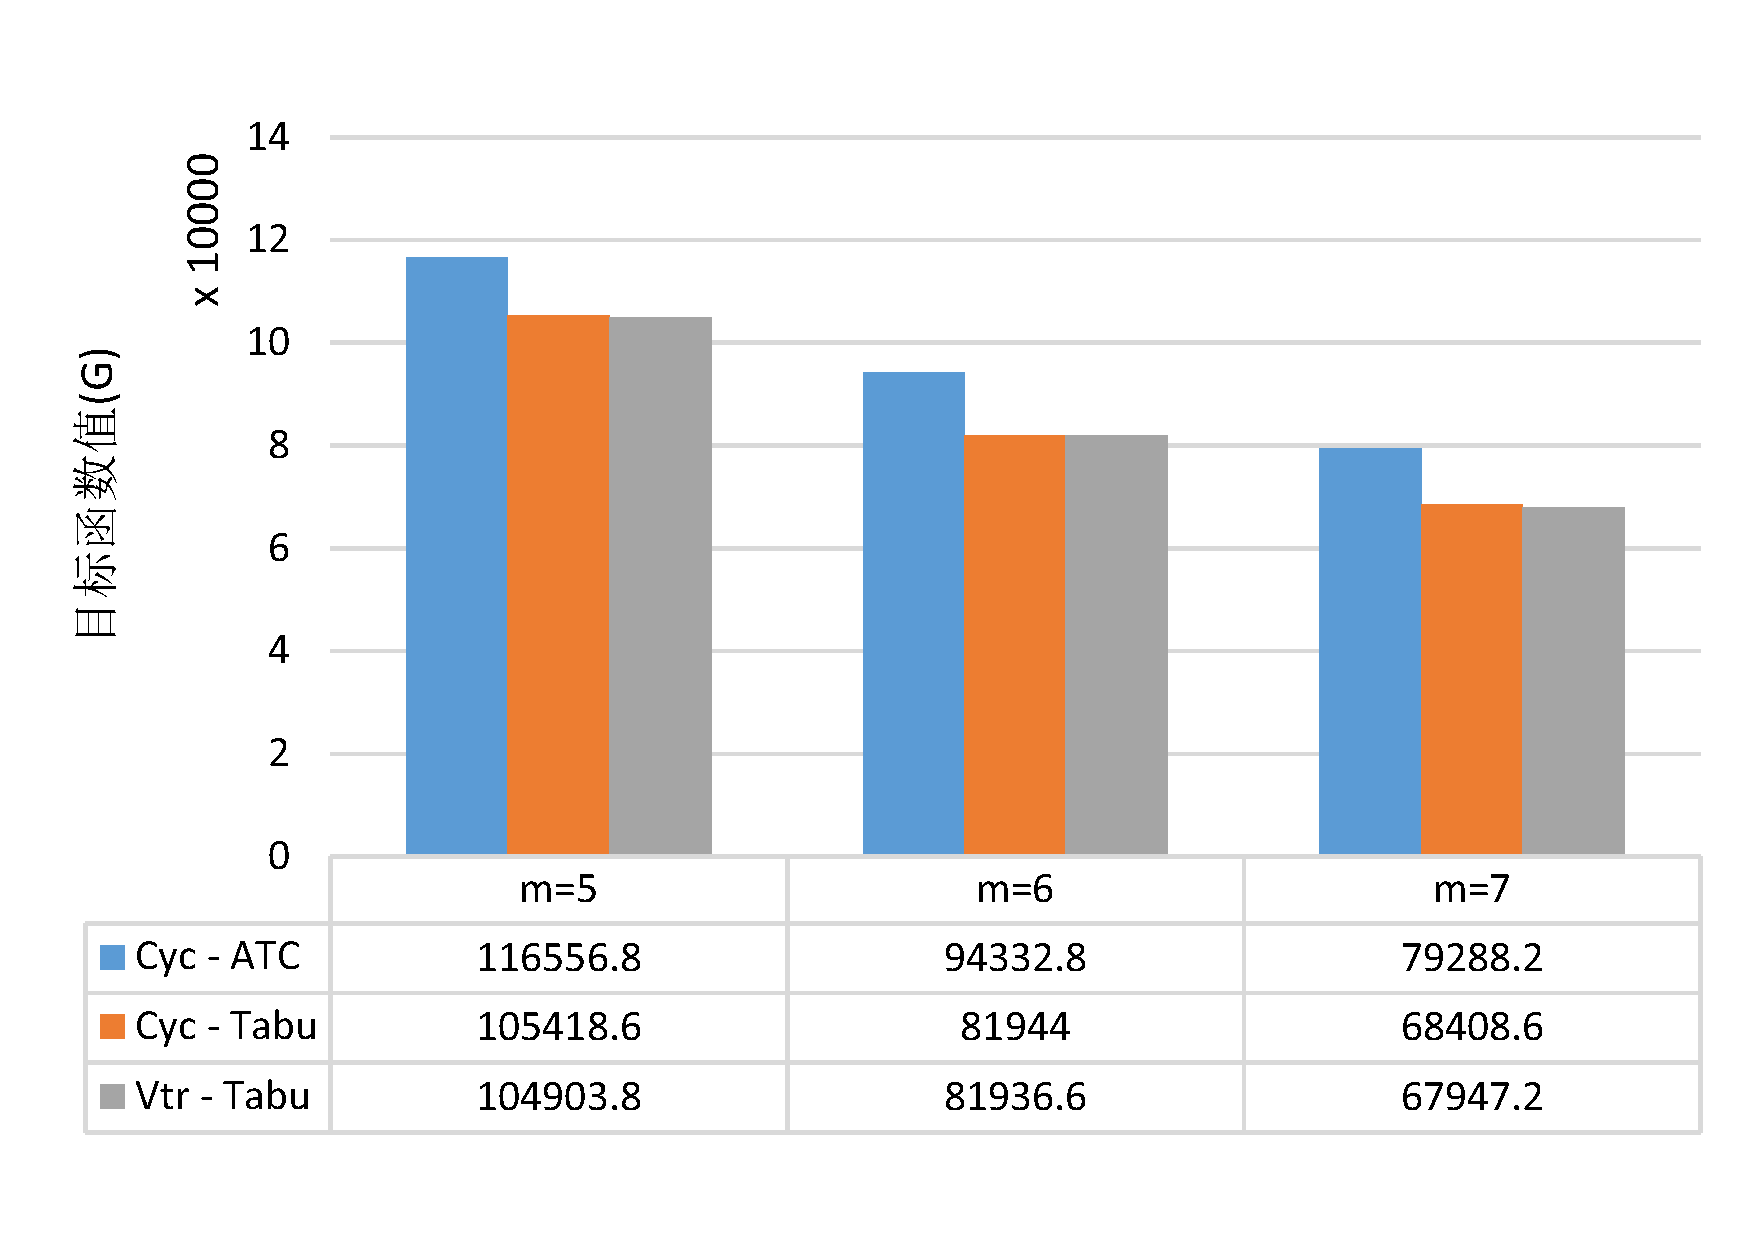
\includegraphics[height = 6cm, angle = -90]{basic_04_100}}
\subfloat[$n = 150$]{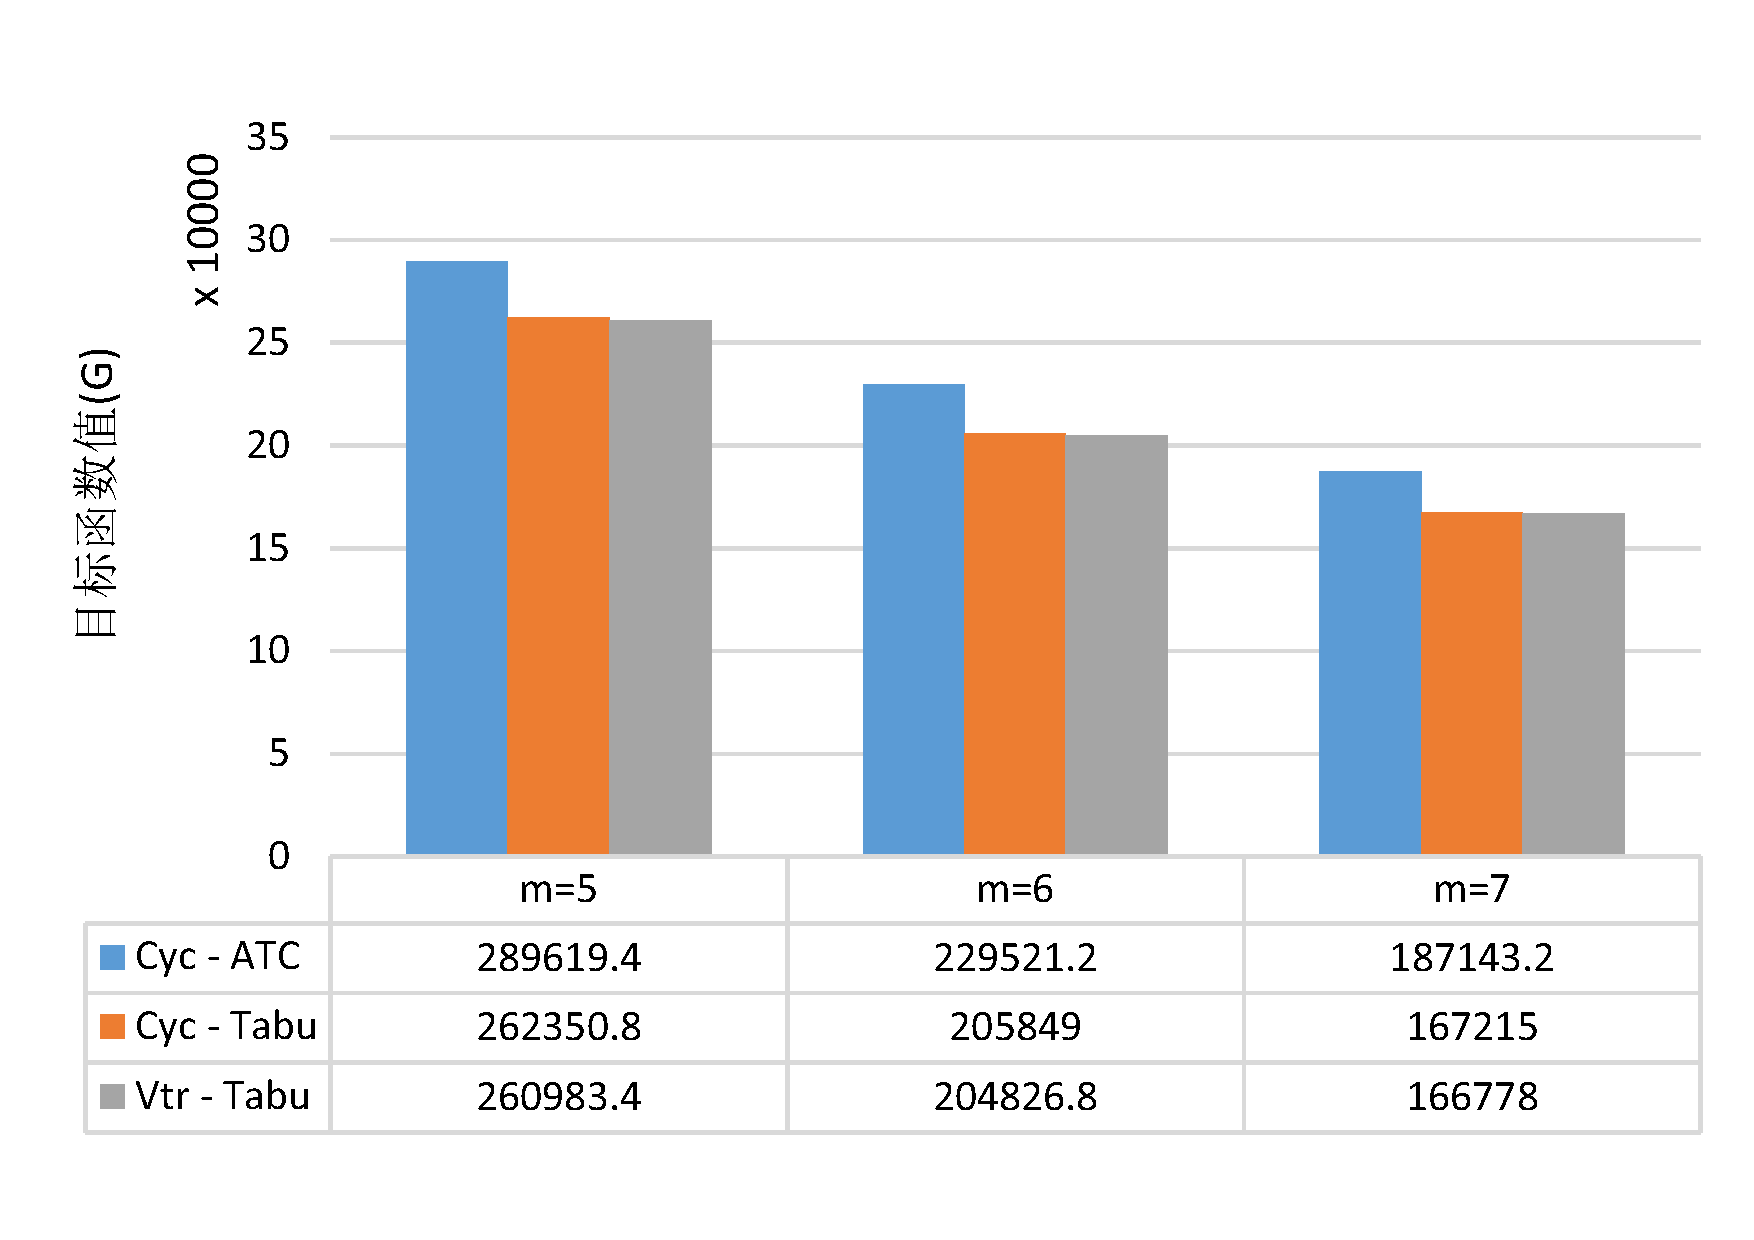
\includegraphics[height = 6cm, angle = -90]{basic_04_150}}
\subfloat[$n = 200$]{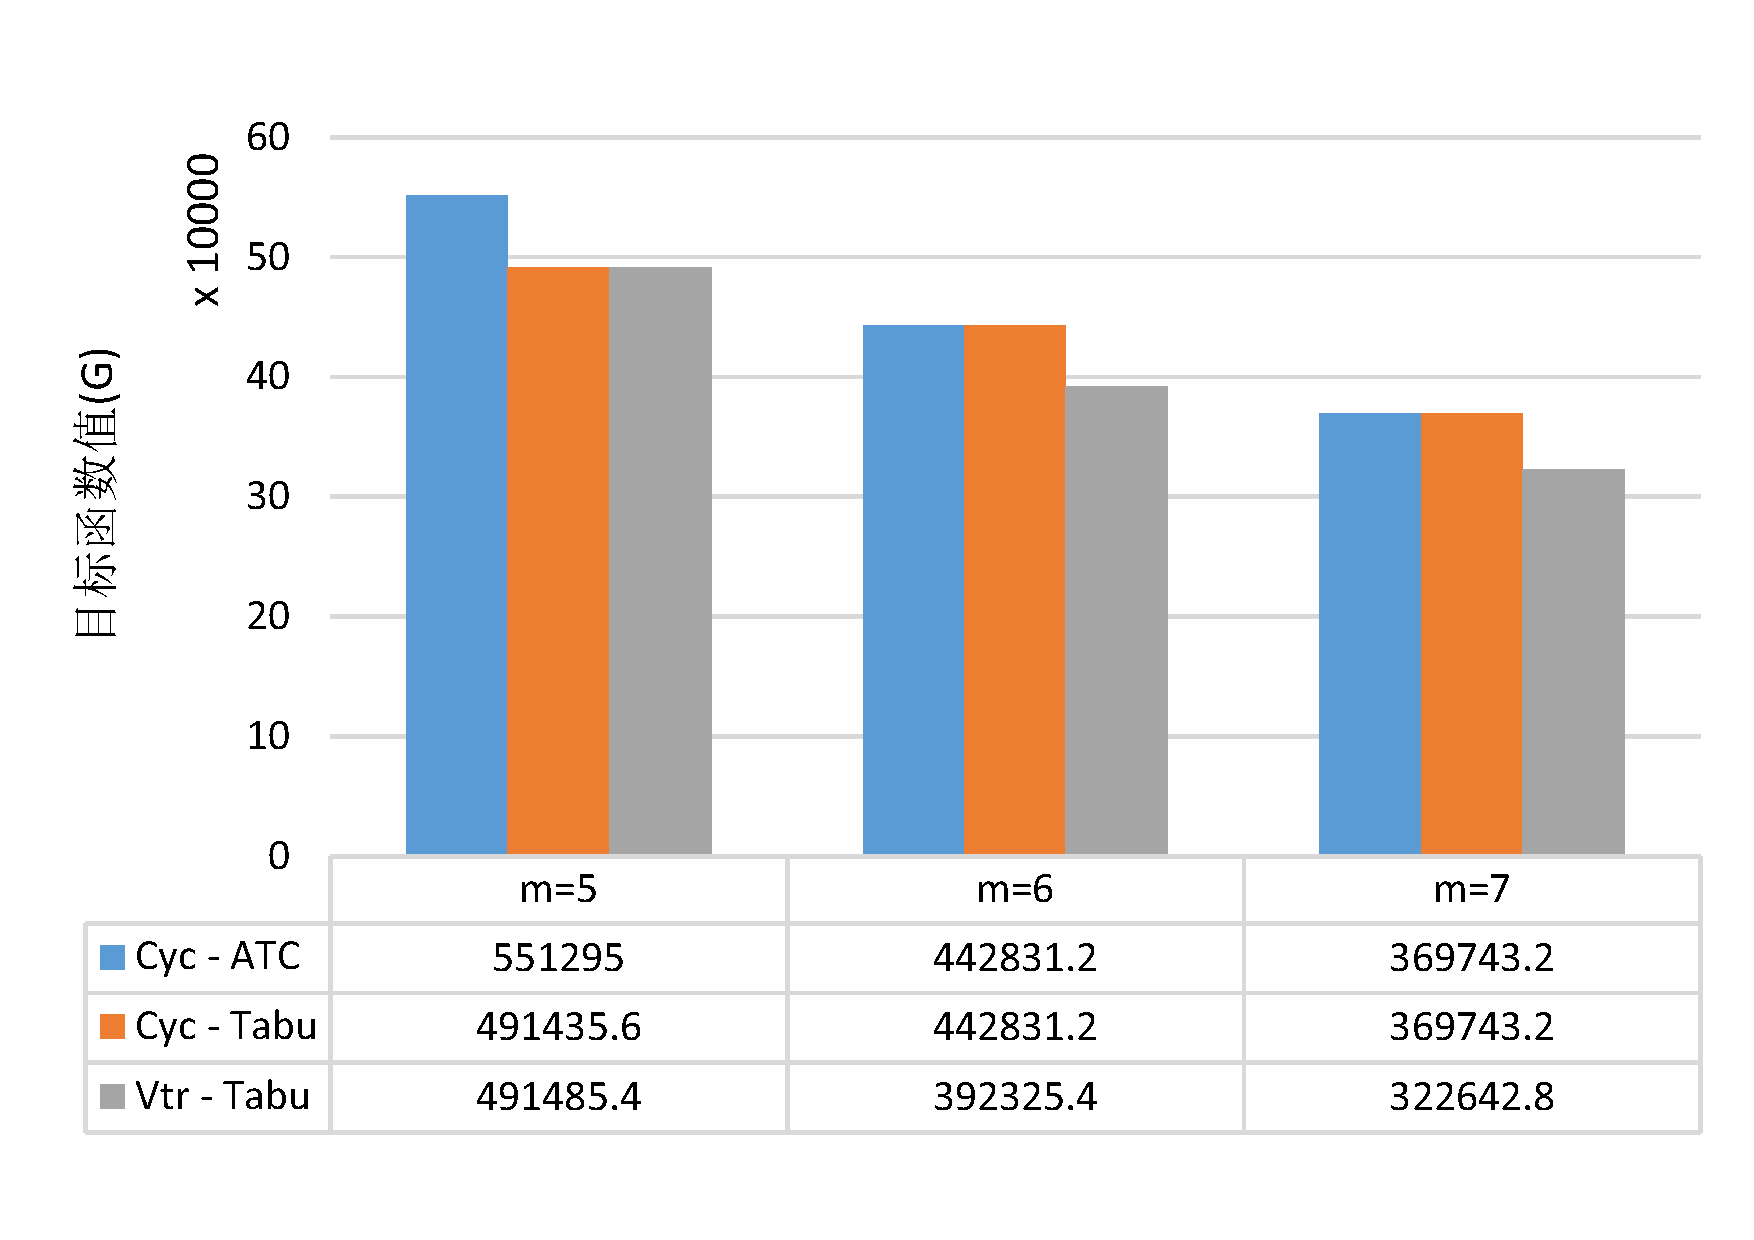
\includegraphics[height = 6cm, angle = -90]{basic_04_200}}
\subfloat[$n = 300$]{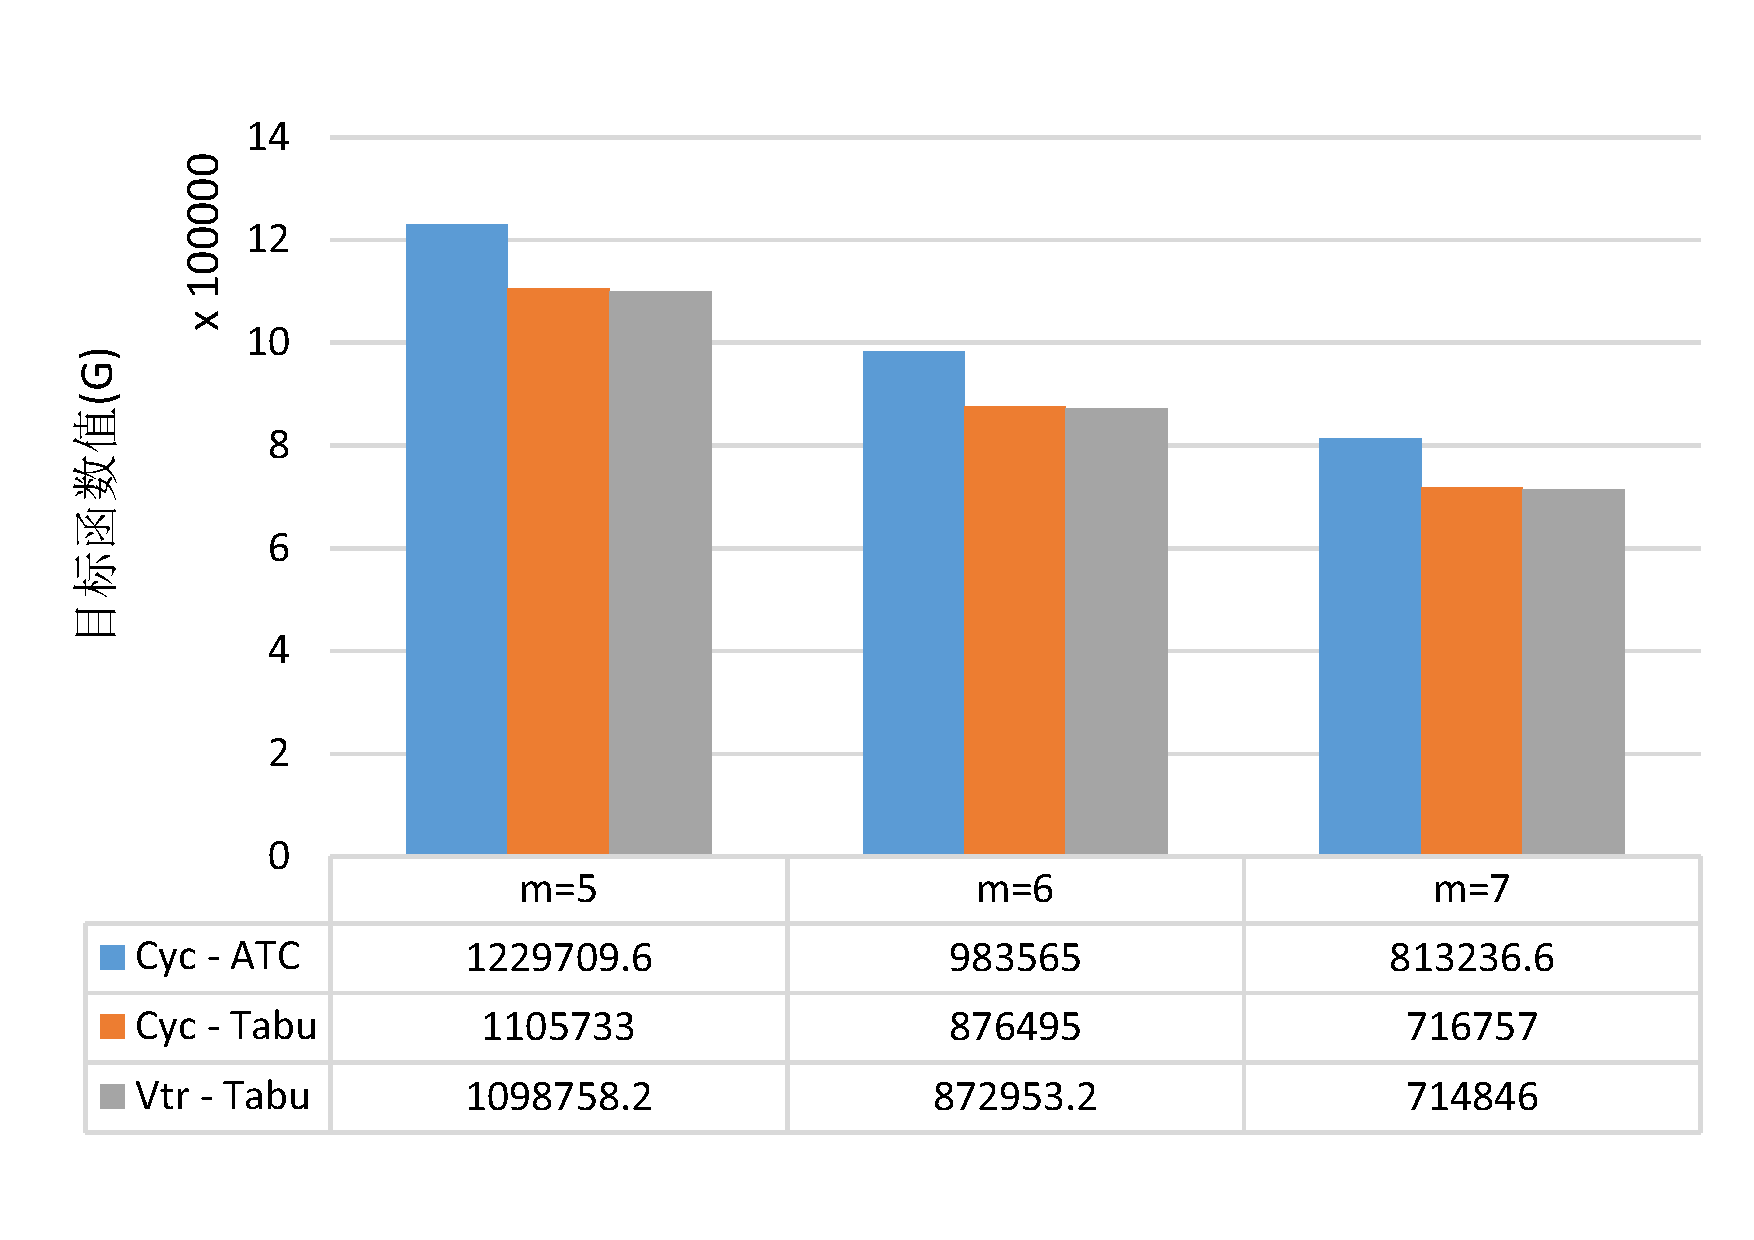
\includegraphics[height = 6cm, angle = -90]{basic_04_300}}\\
\subfloat[$n = 500$]{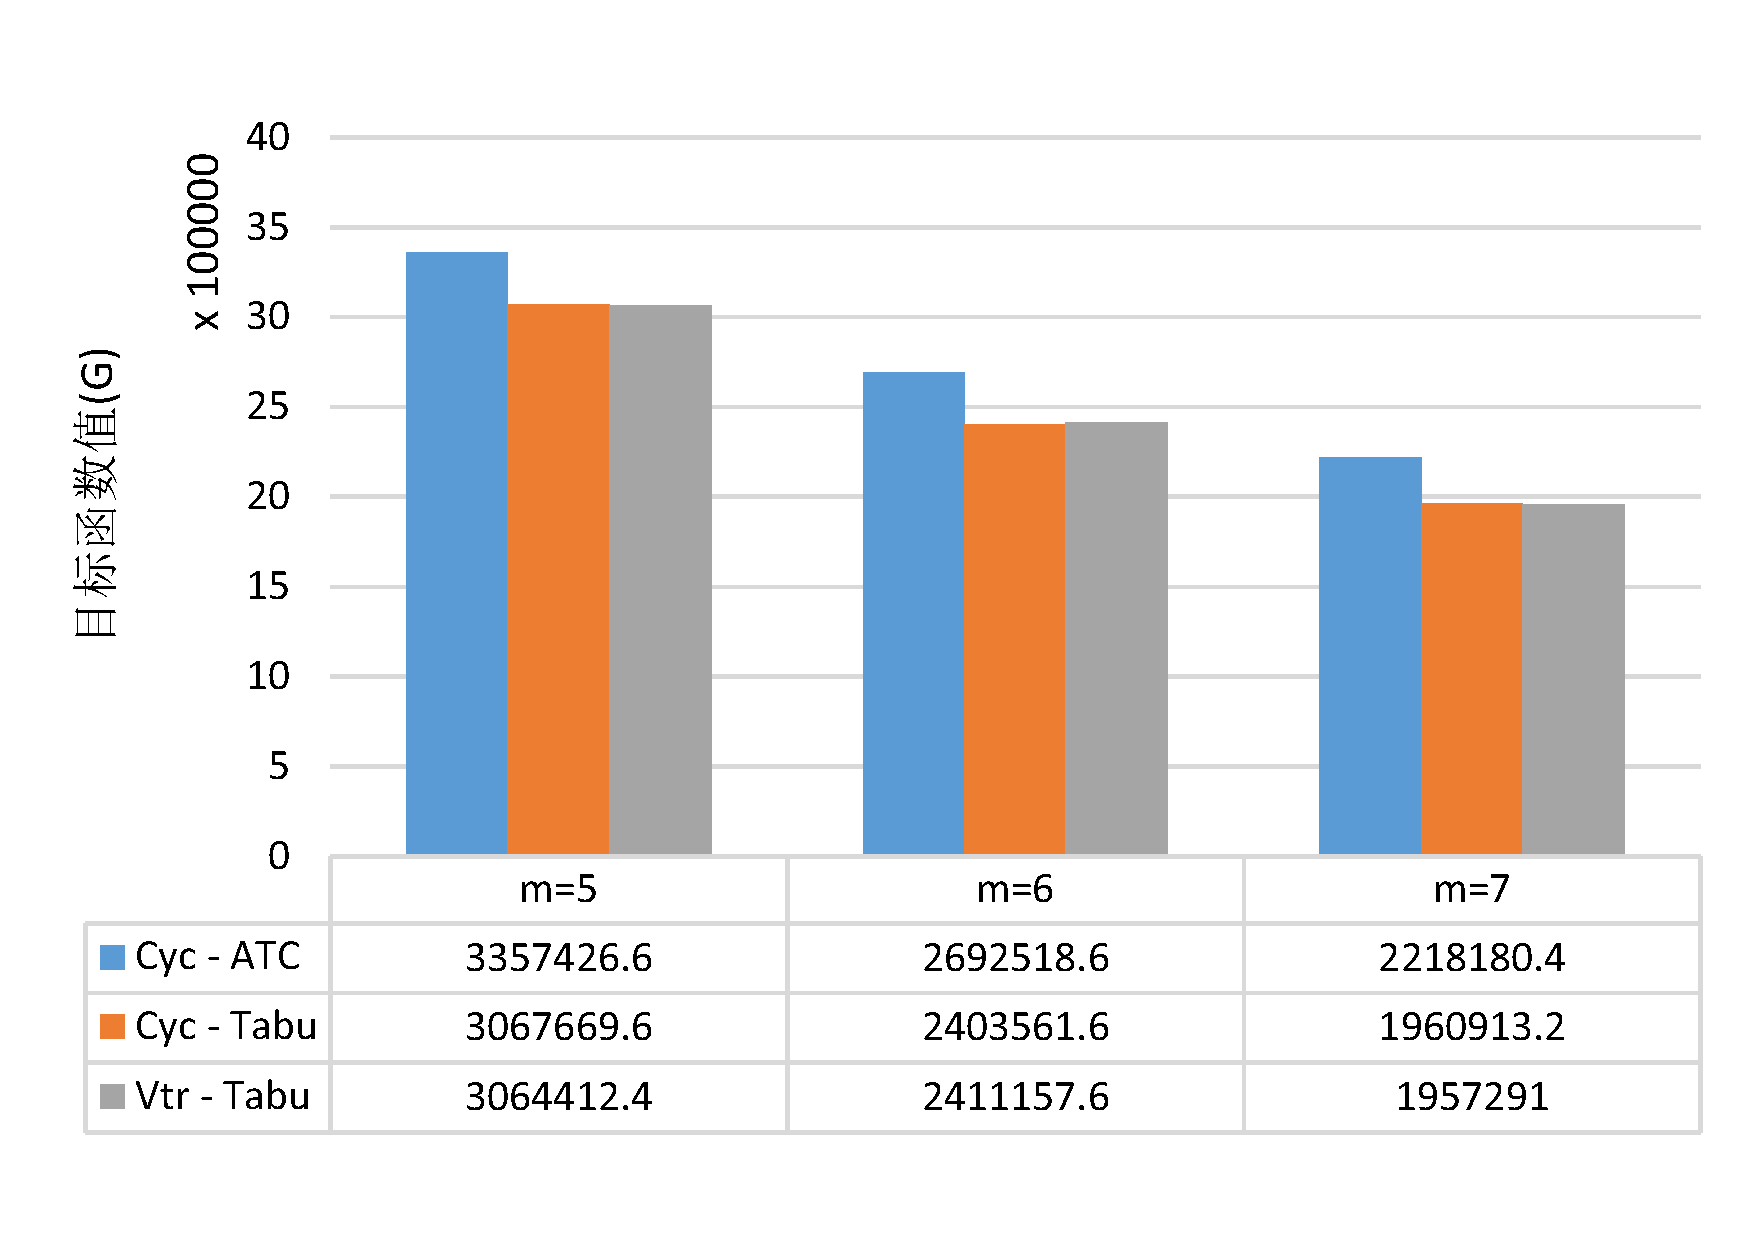
\includegraphics[height = 6cm, angle = -90]{basic_04_500}}
\subfloat[$n = 750$]{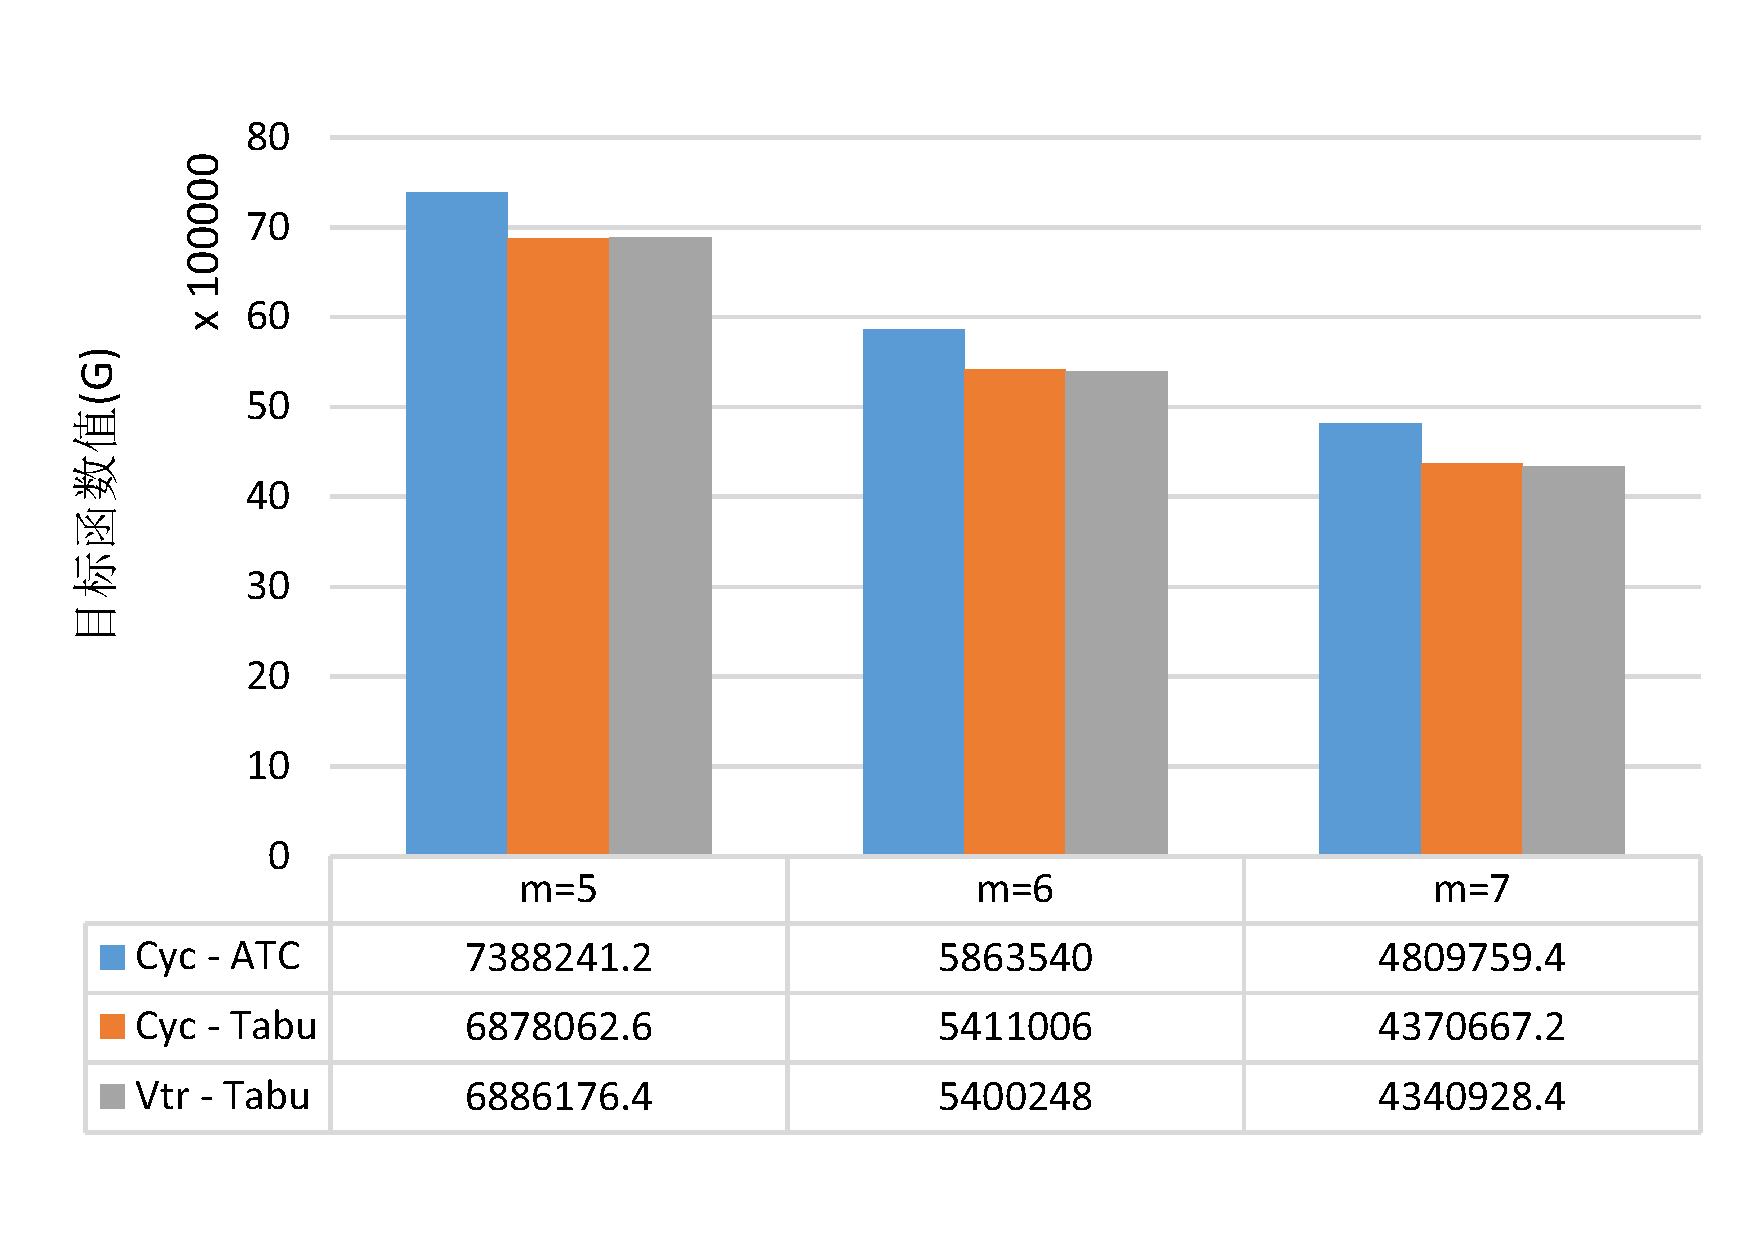
\includegraphics[height = 6cm, angle = -90]{basic_04_750}}
\subfloat[$n = 1000$]{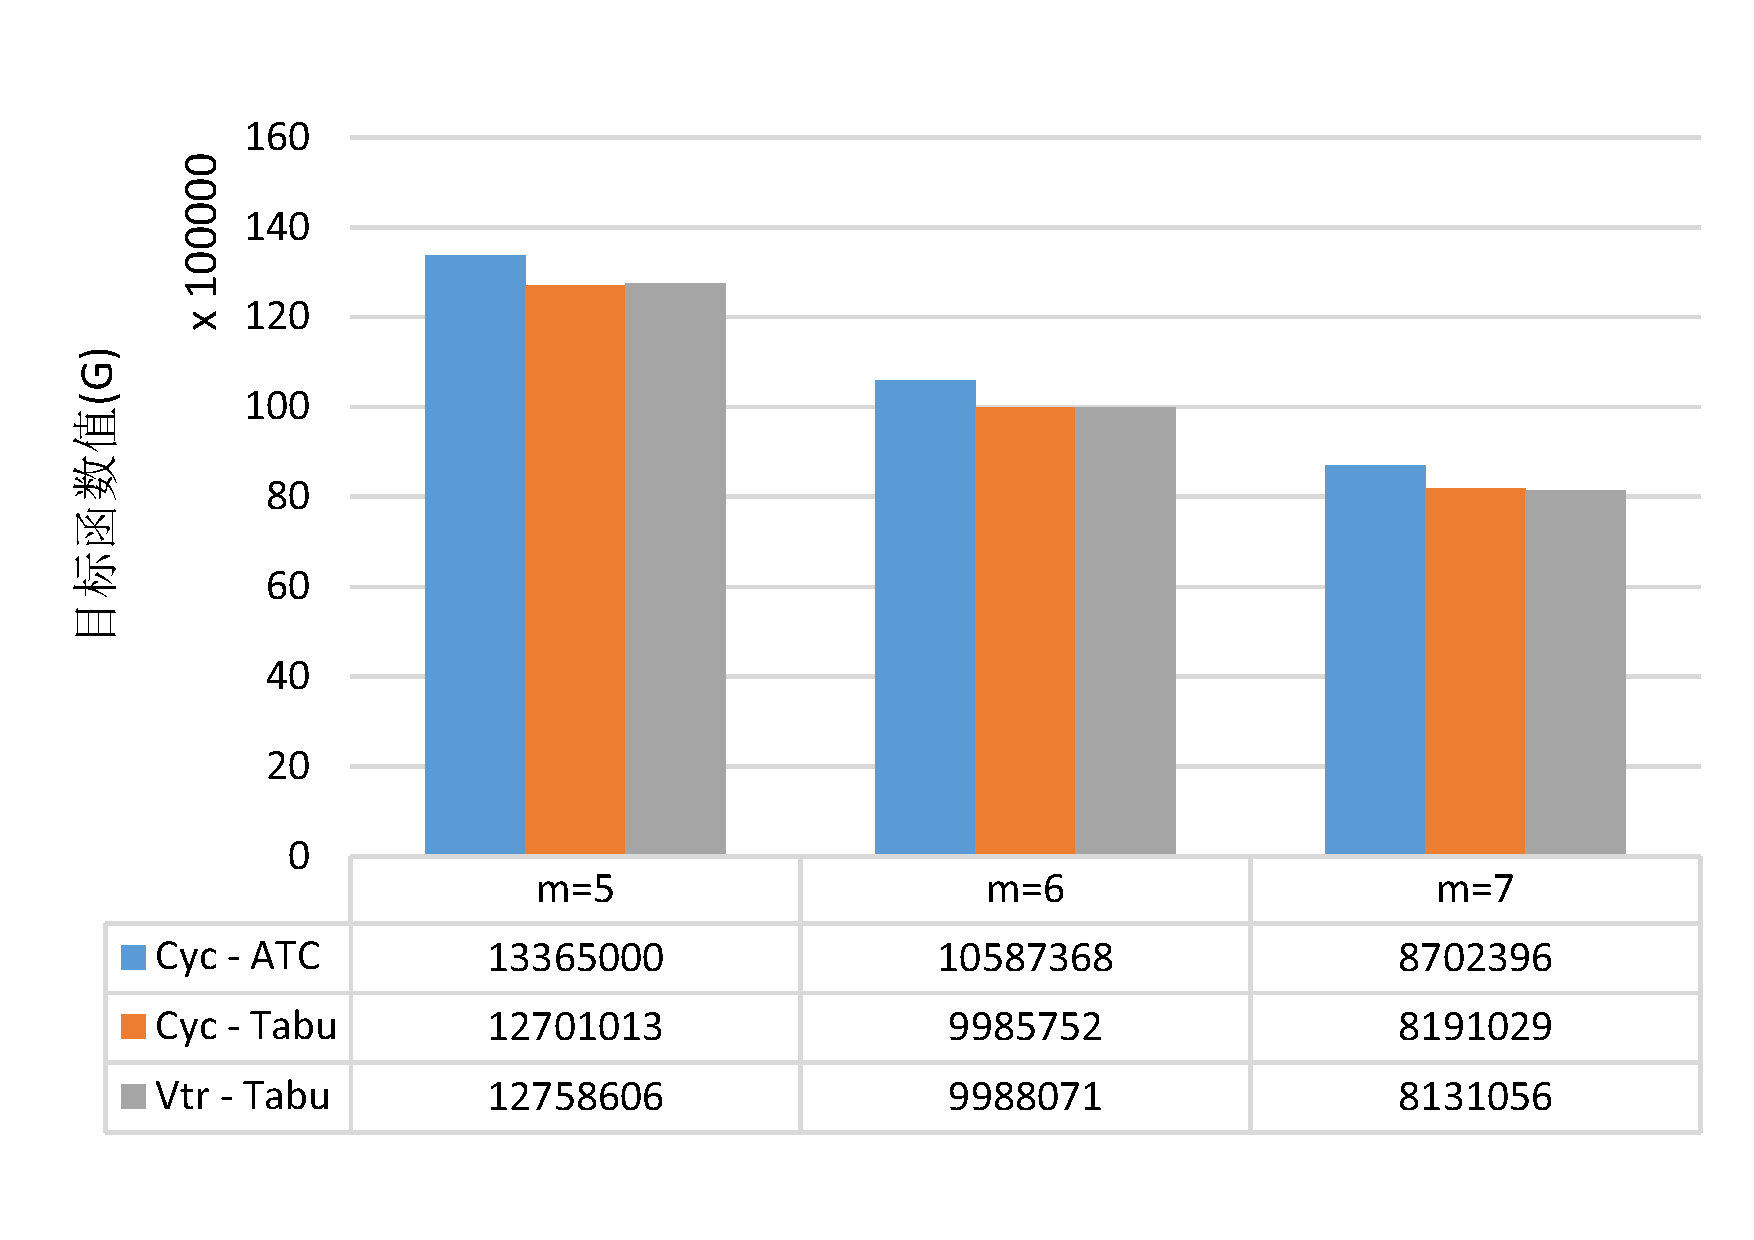
\includegraphics[height = 6cm, angle = -90]{basic_04_1000}}
\caption{\label{fig:result1}模型$1$的Cyc -- ATC、Cyc -- Tabu、Vtr -- Tabu 算法求解目标函数值比较$(\lambda_1 = 0.4)$}
\end{sidewaysfigure}

\begin{sidewaysfigure}
\centering
\subfloat[$n = 20$]{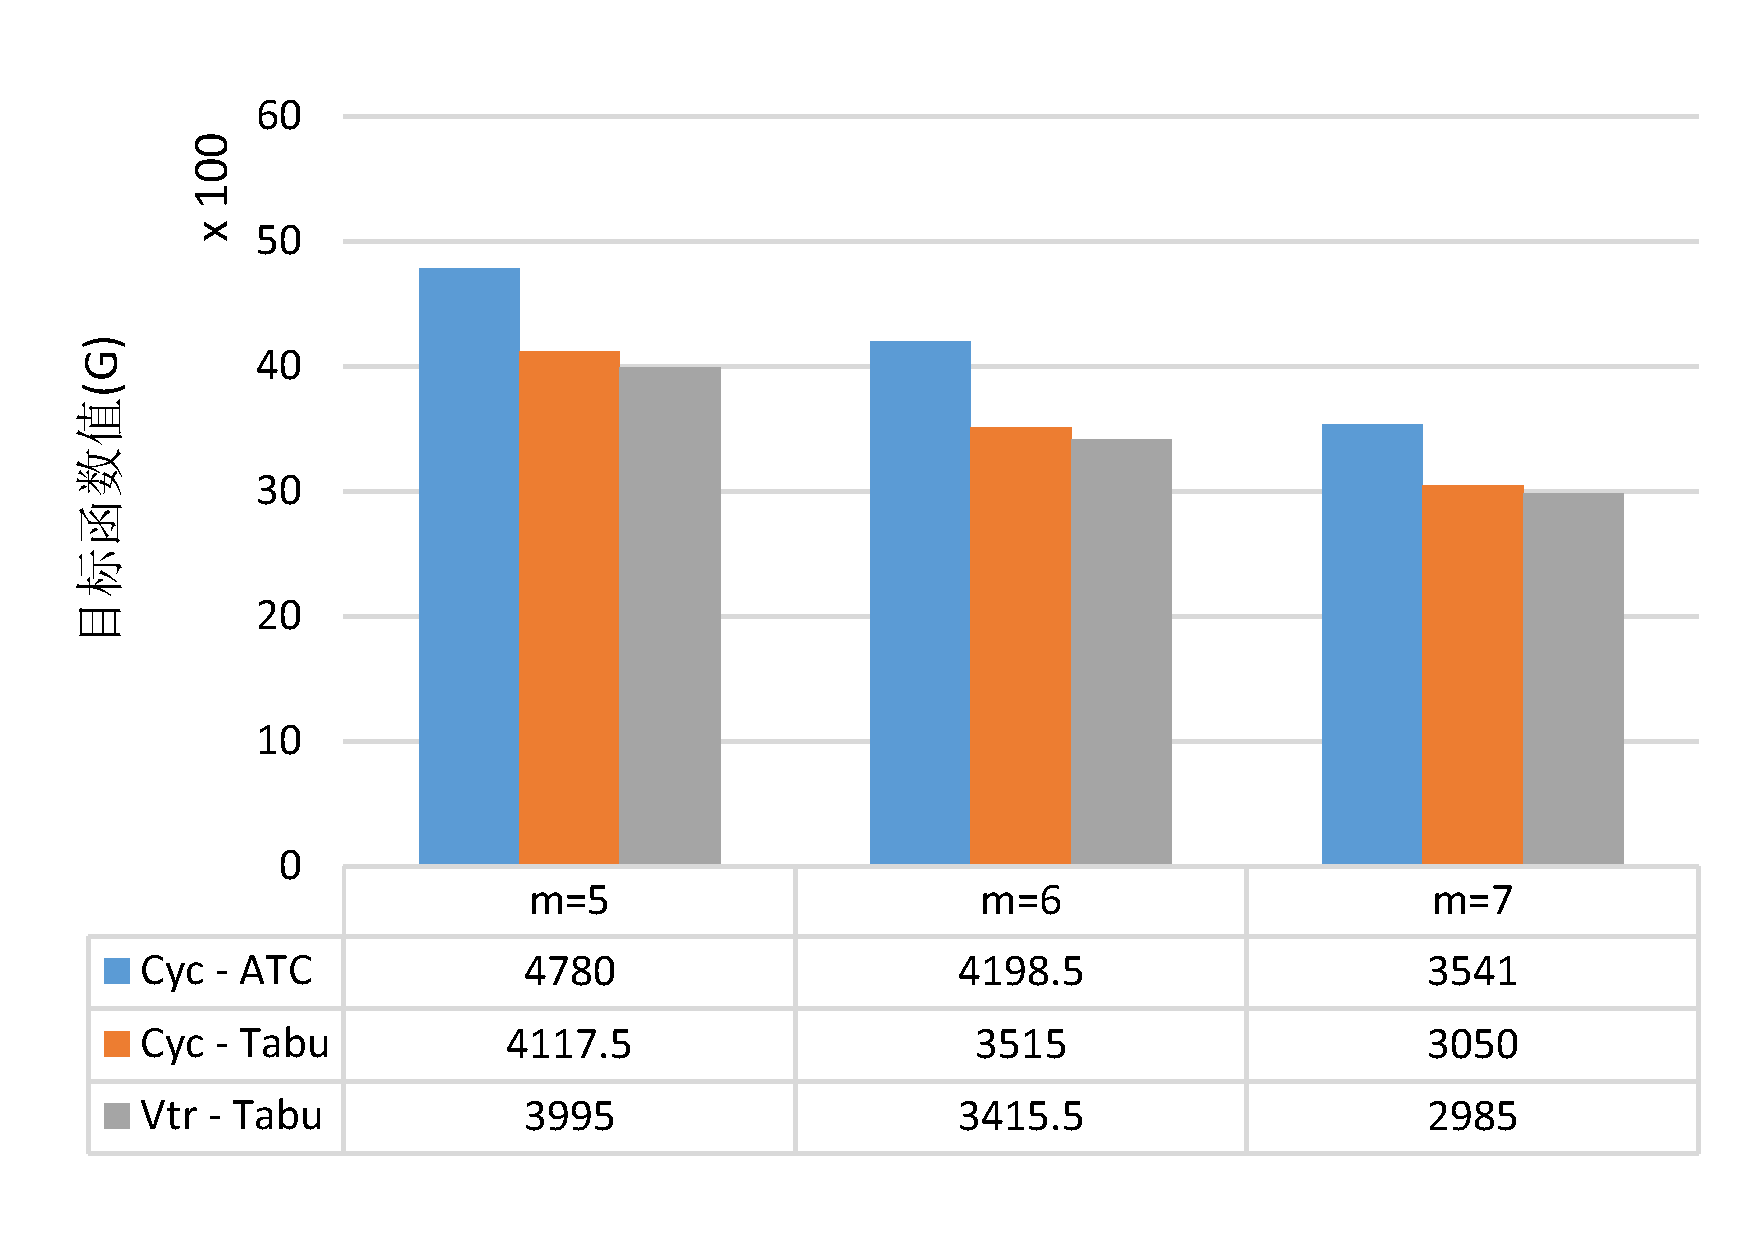
\includegraphics[height = 6cm, angle = -90]{basic_05_20}}
\subfloat[$n = 30$]{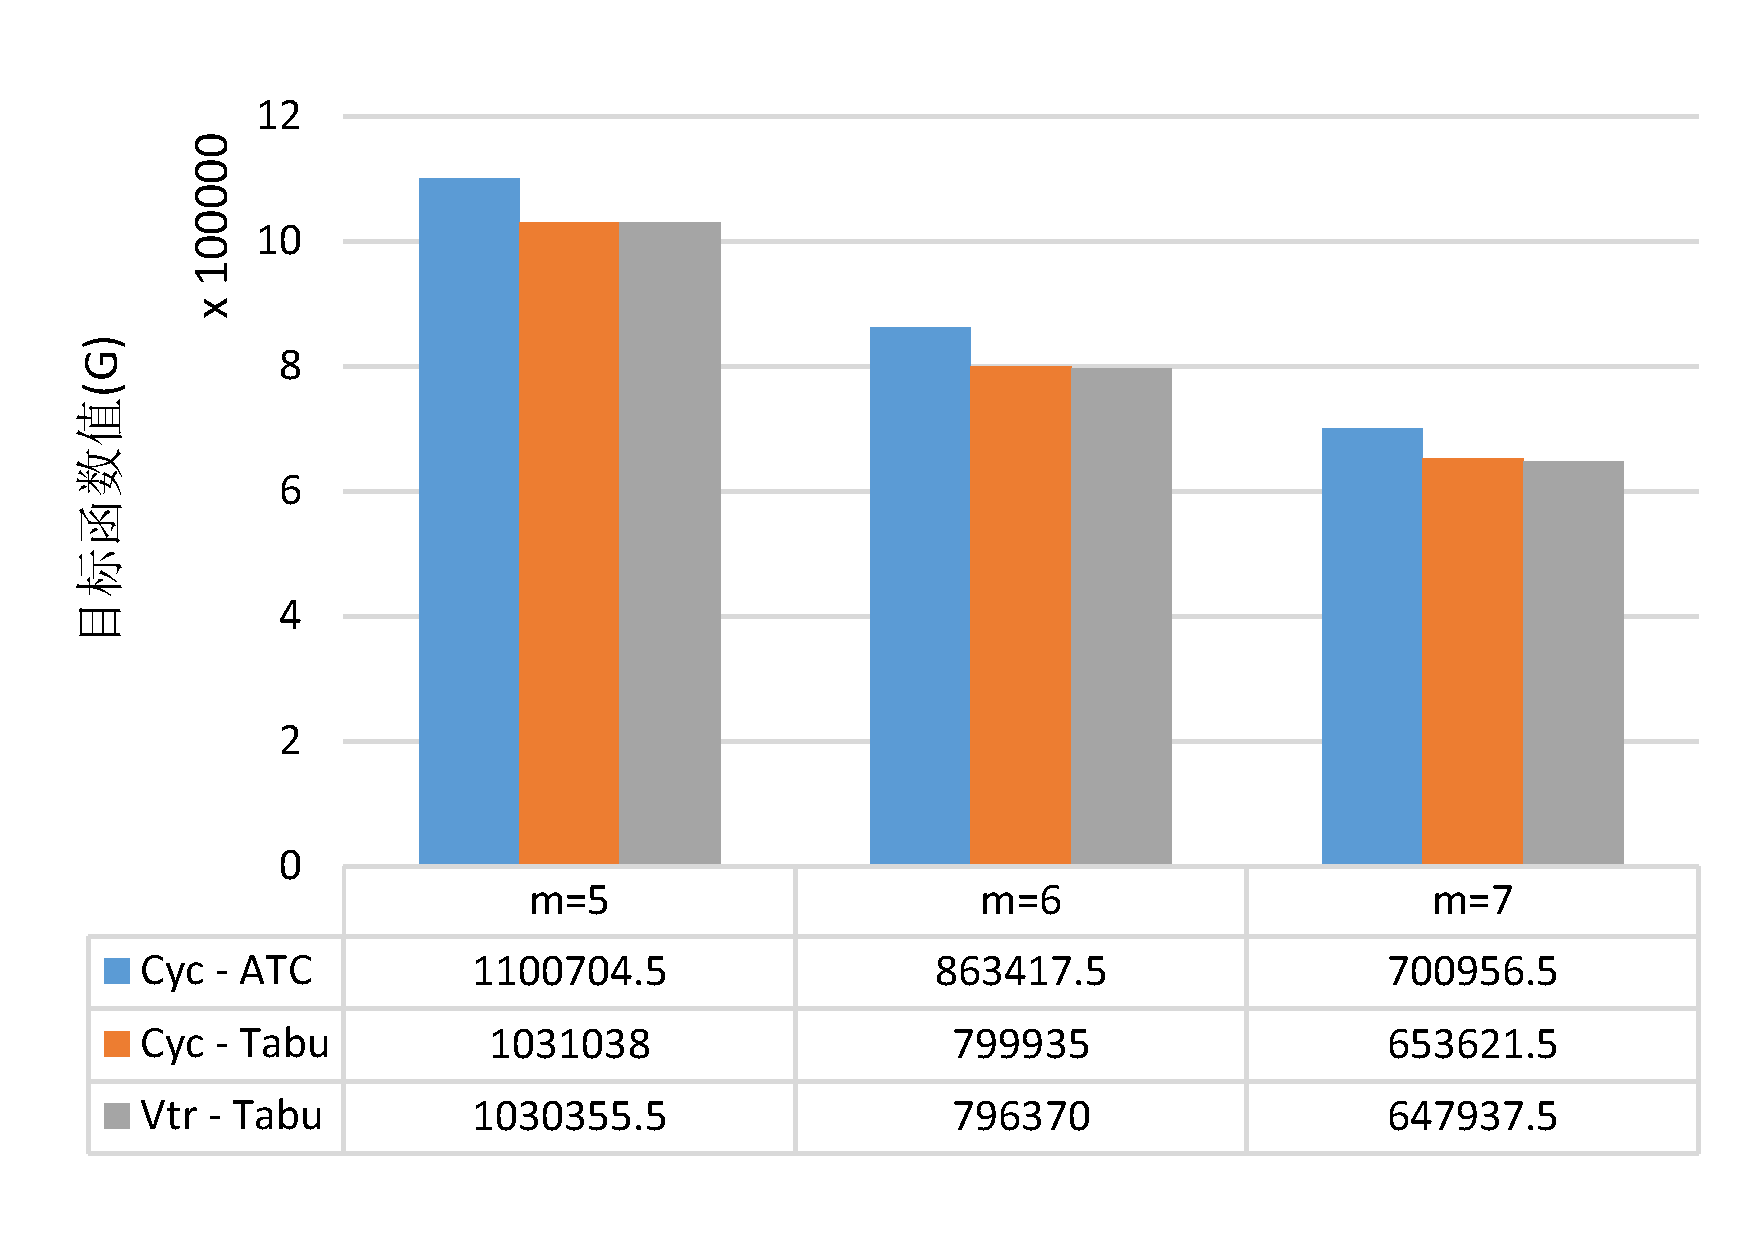
\includegraphics[height = 6cm, angle = -90]{basic_05_300}}
\subfloat[$n = 50$]{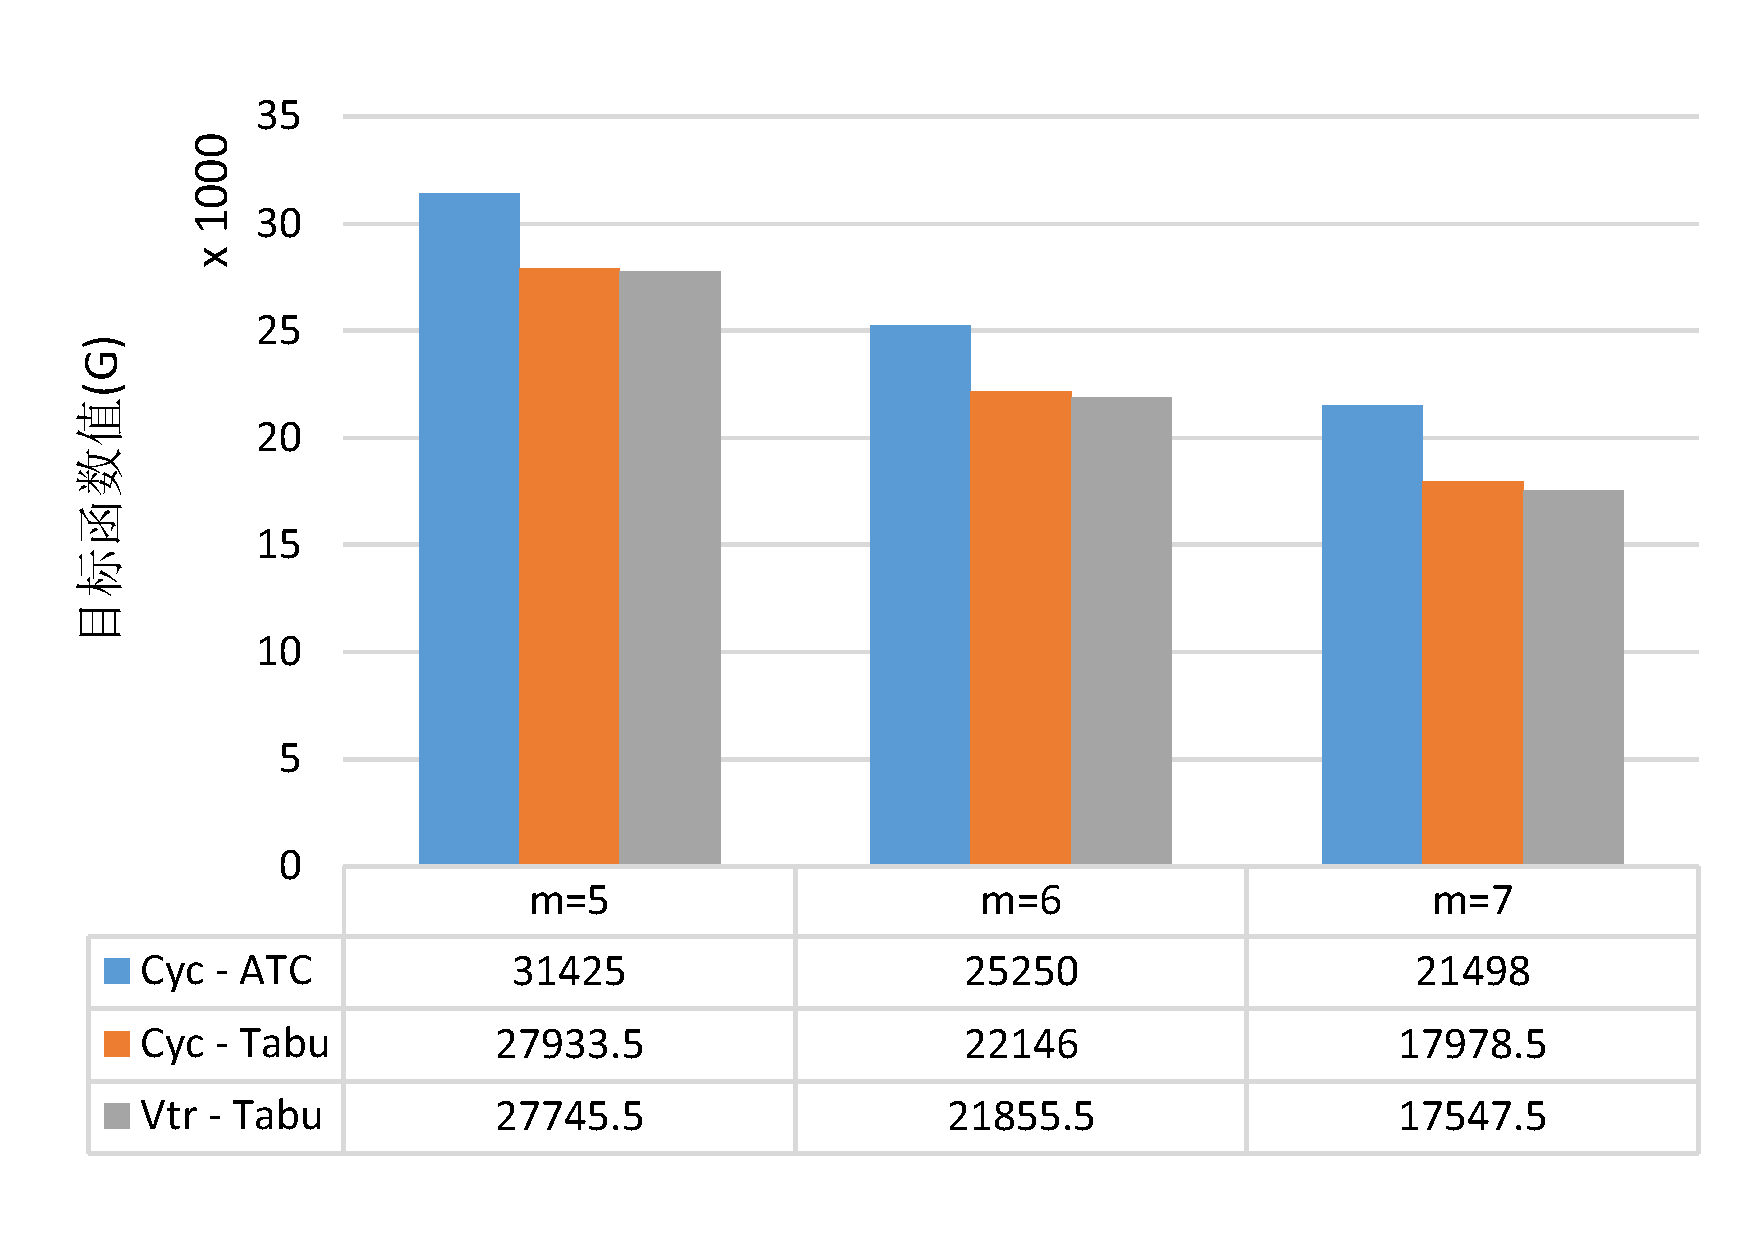
\includegraphics[height = 6cm, angle = -90]{basic_05_50}}
\subfloat[$n = 70$]{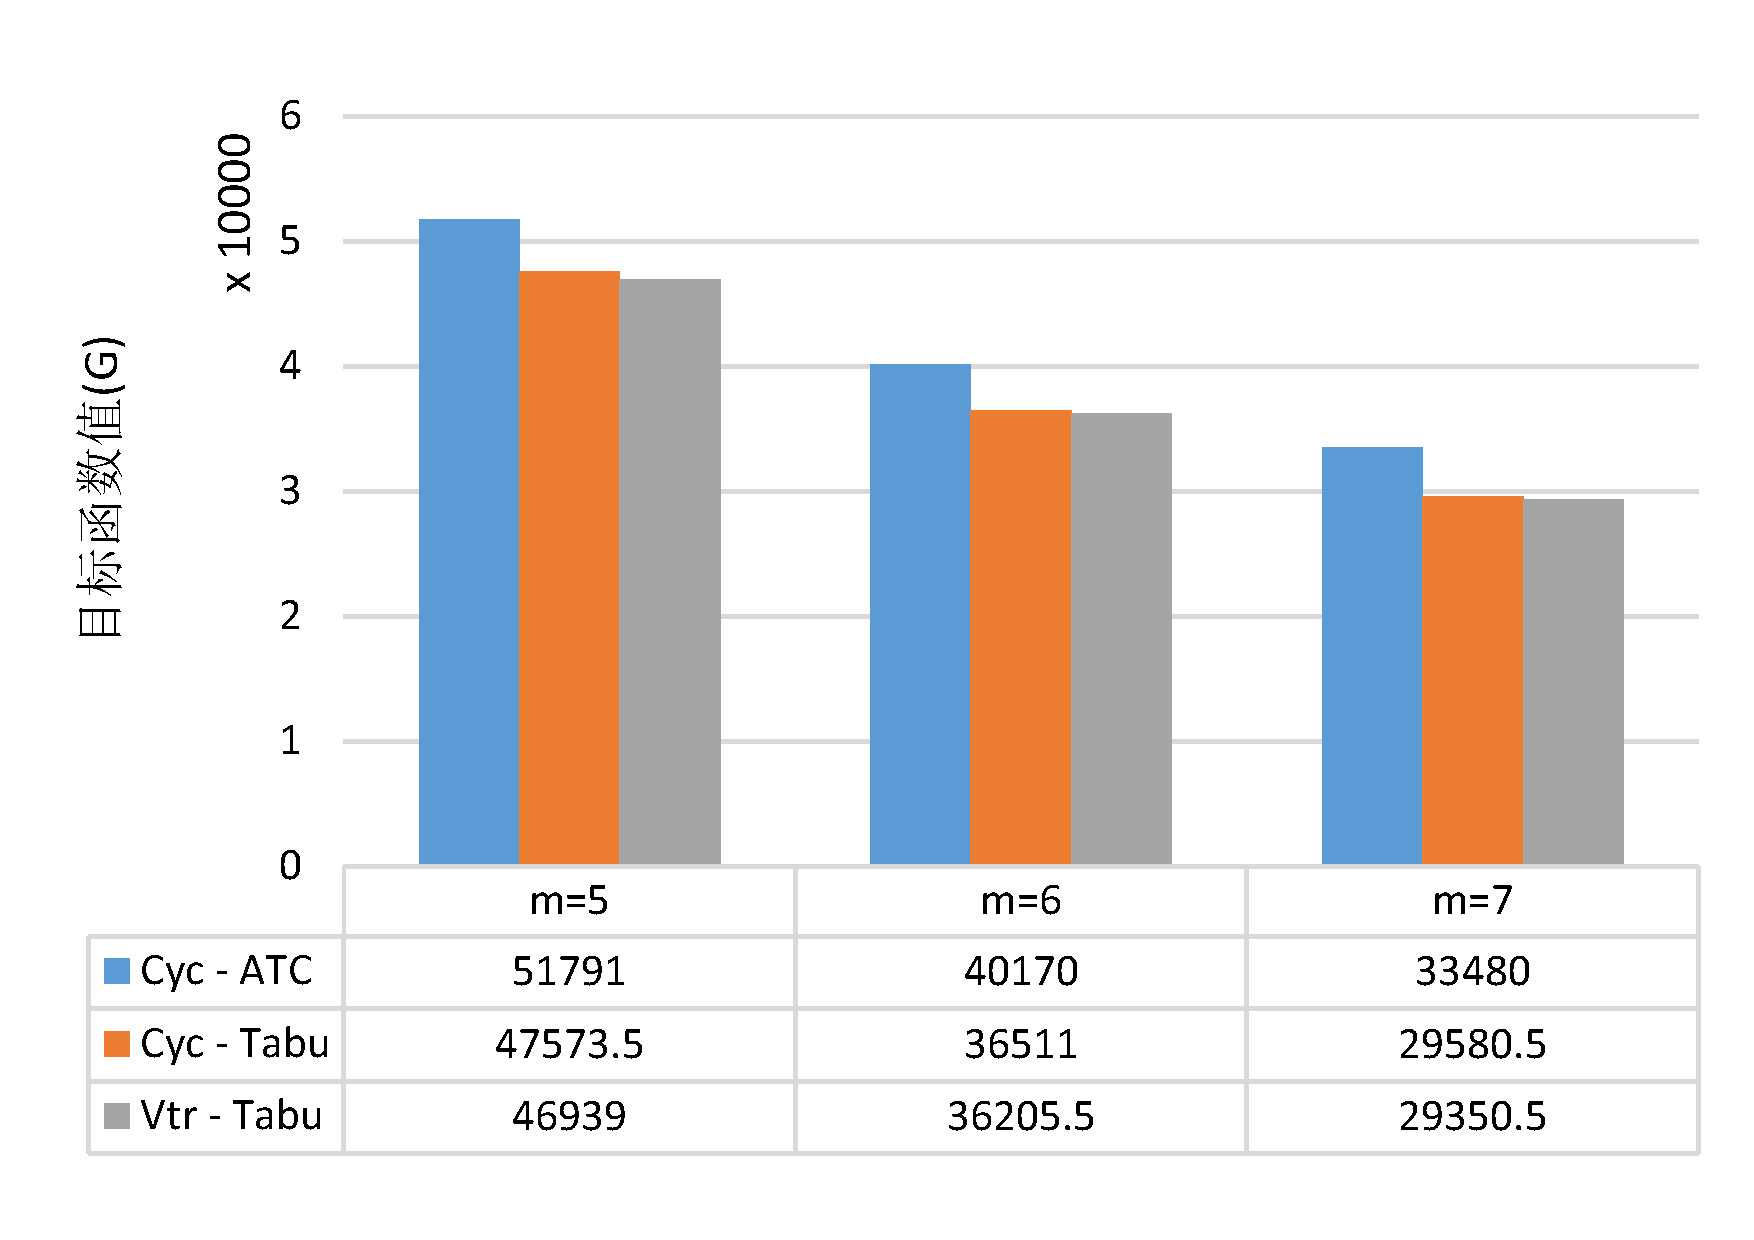
\includegraphics[height = 6cm, angle = -90]{basic_05_70}}\\
\subfloat[$n = 100$]{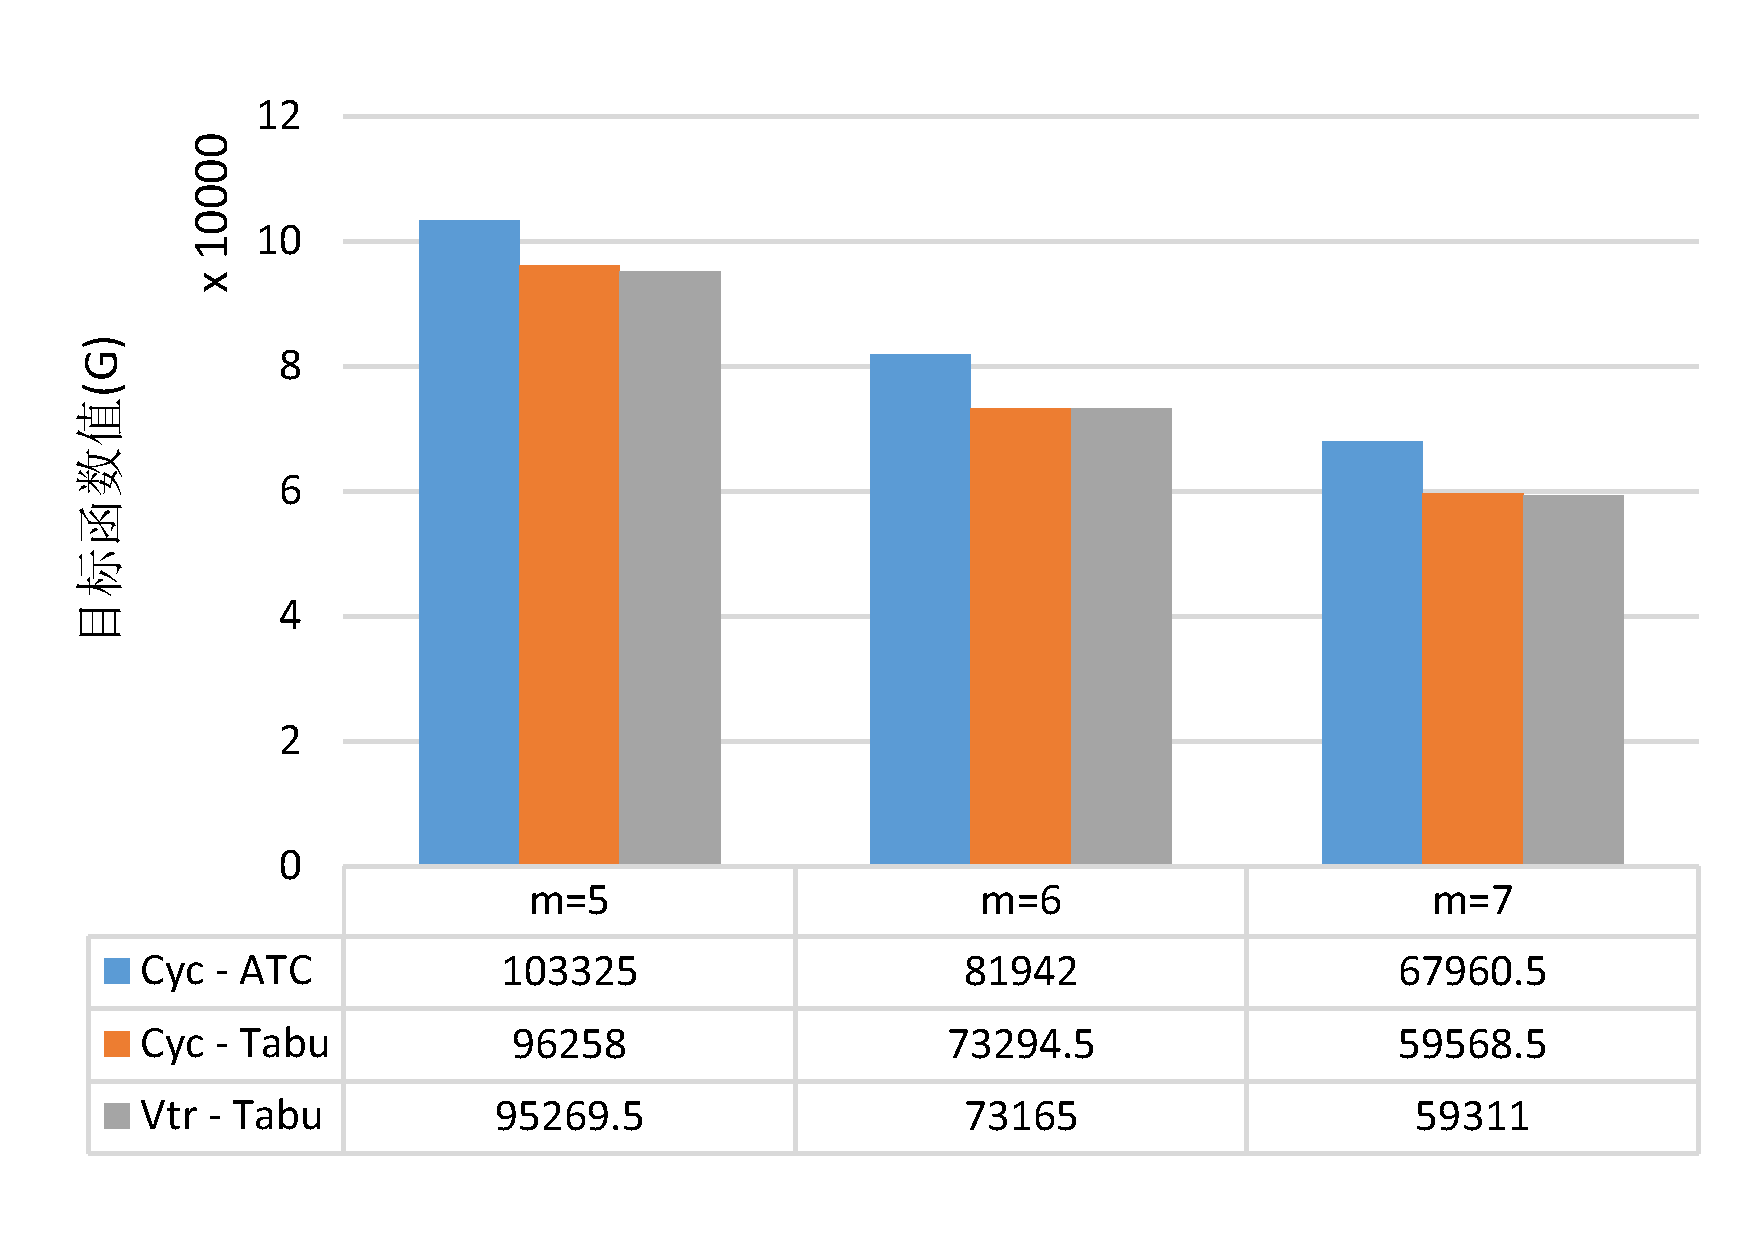
\includegraphics[height = 6cm, angle = -90]{basic_05_100}}
\subfloat[$n = 150$]{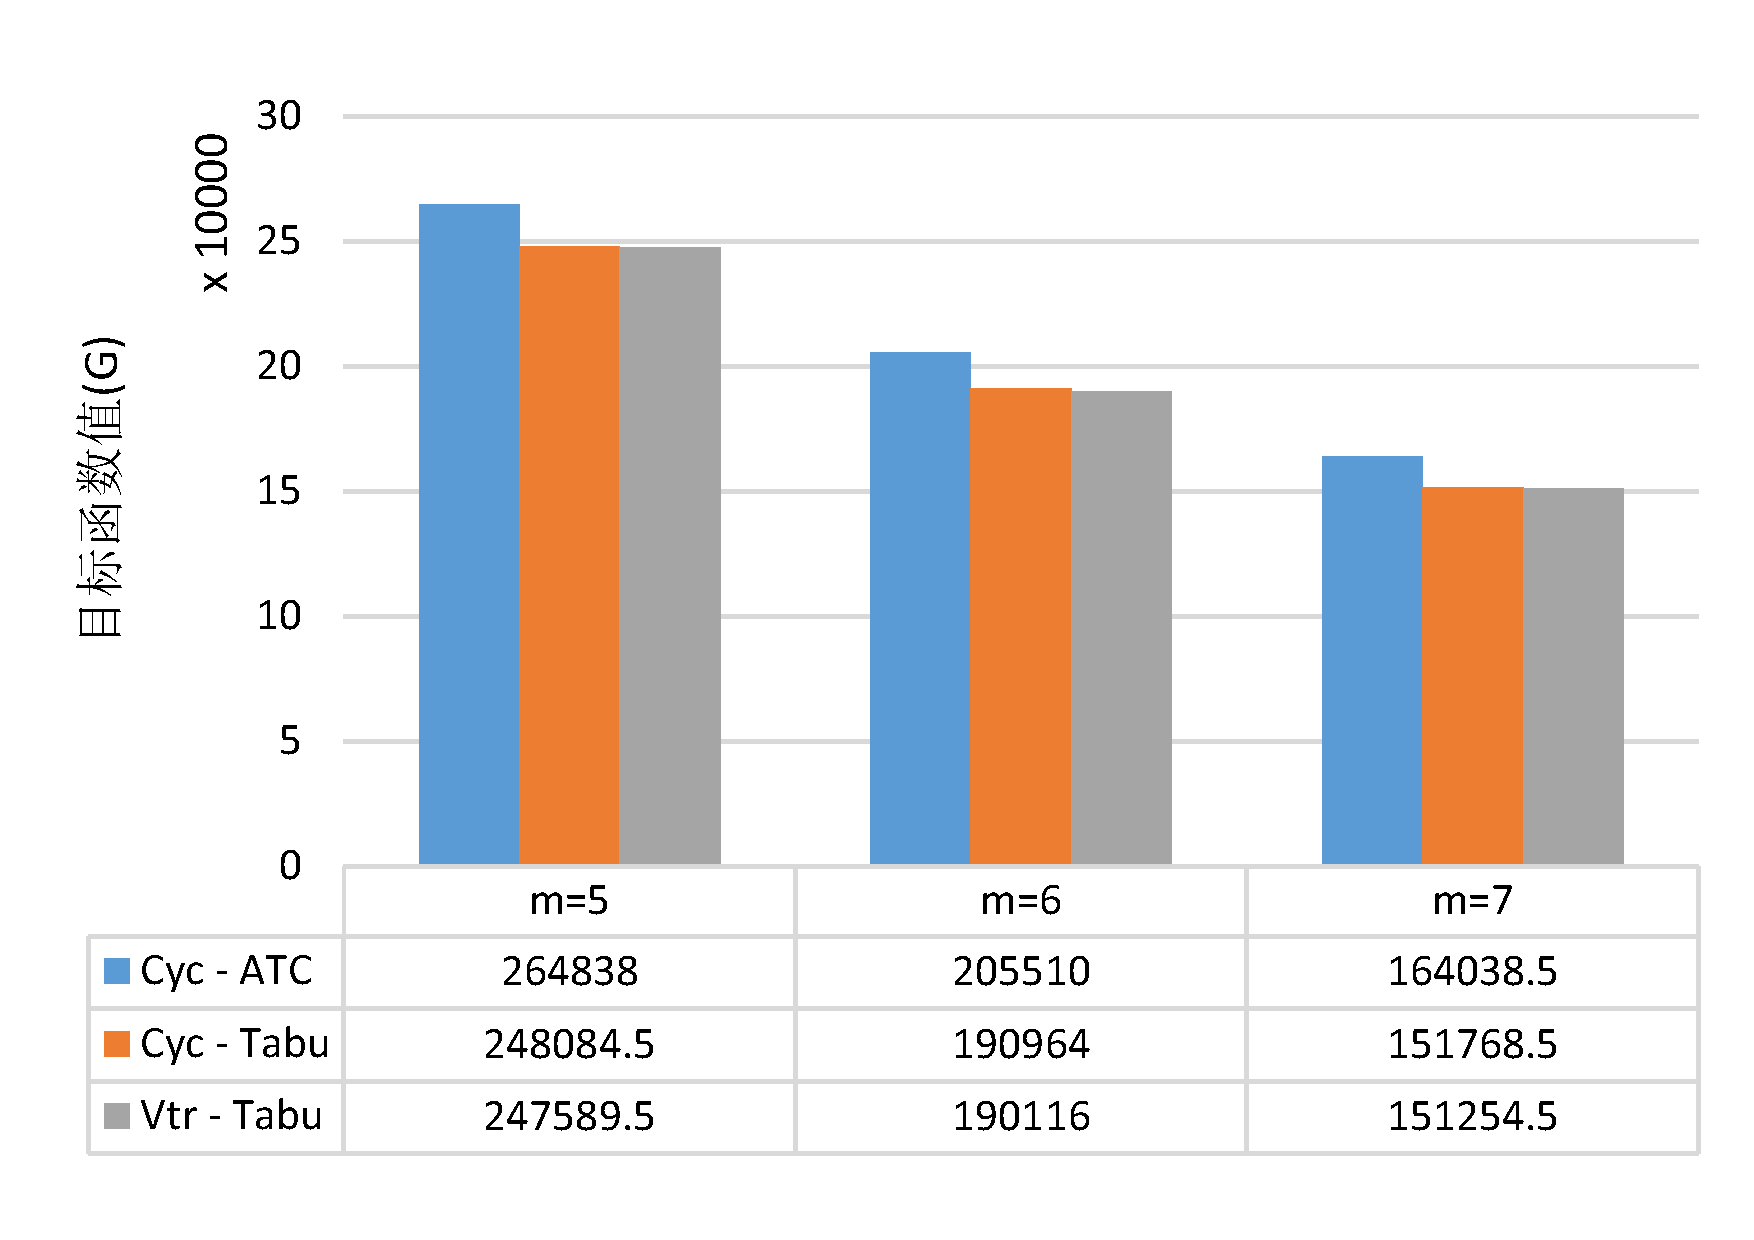
\includegraphics[height = 6cm, angle = -90]{basic_05_150}}
\subfloat[$n = 200$]{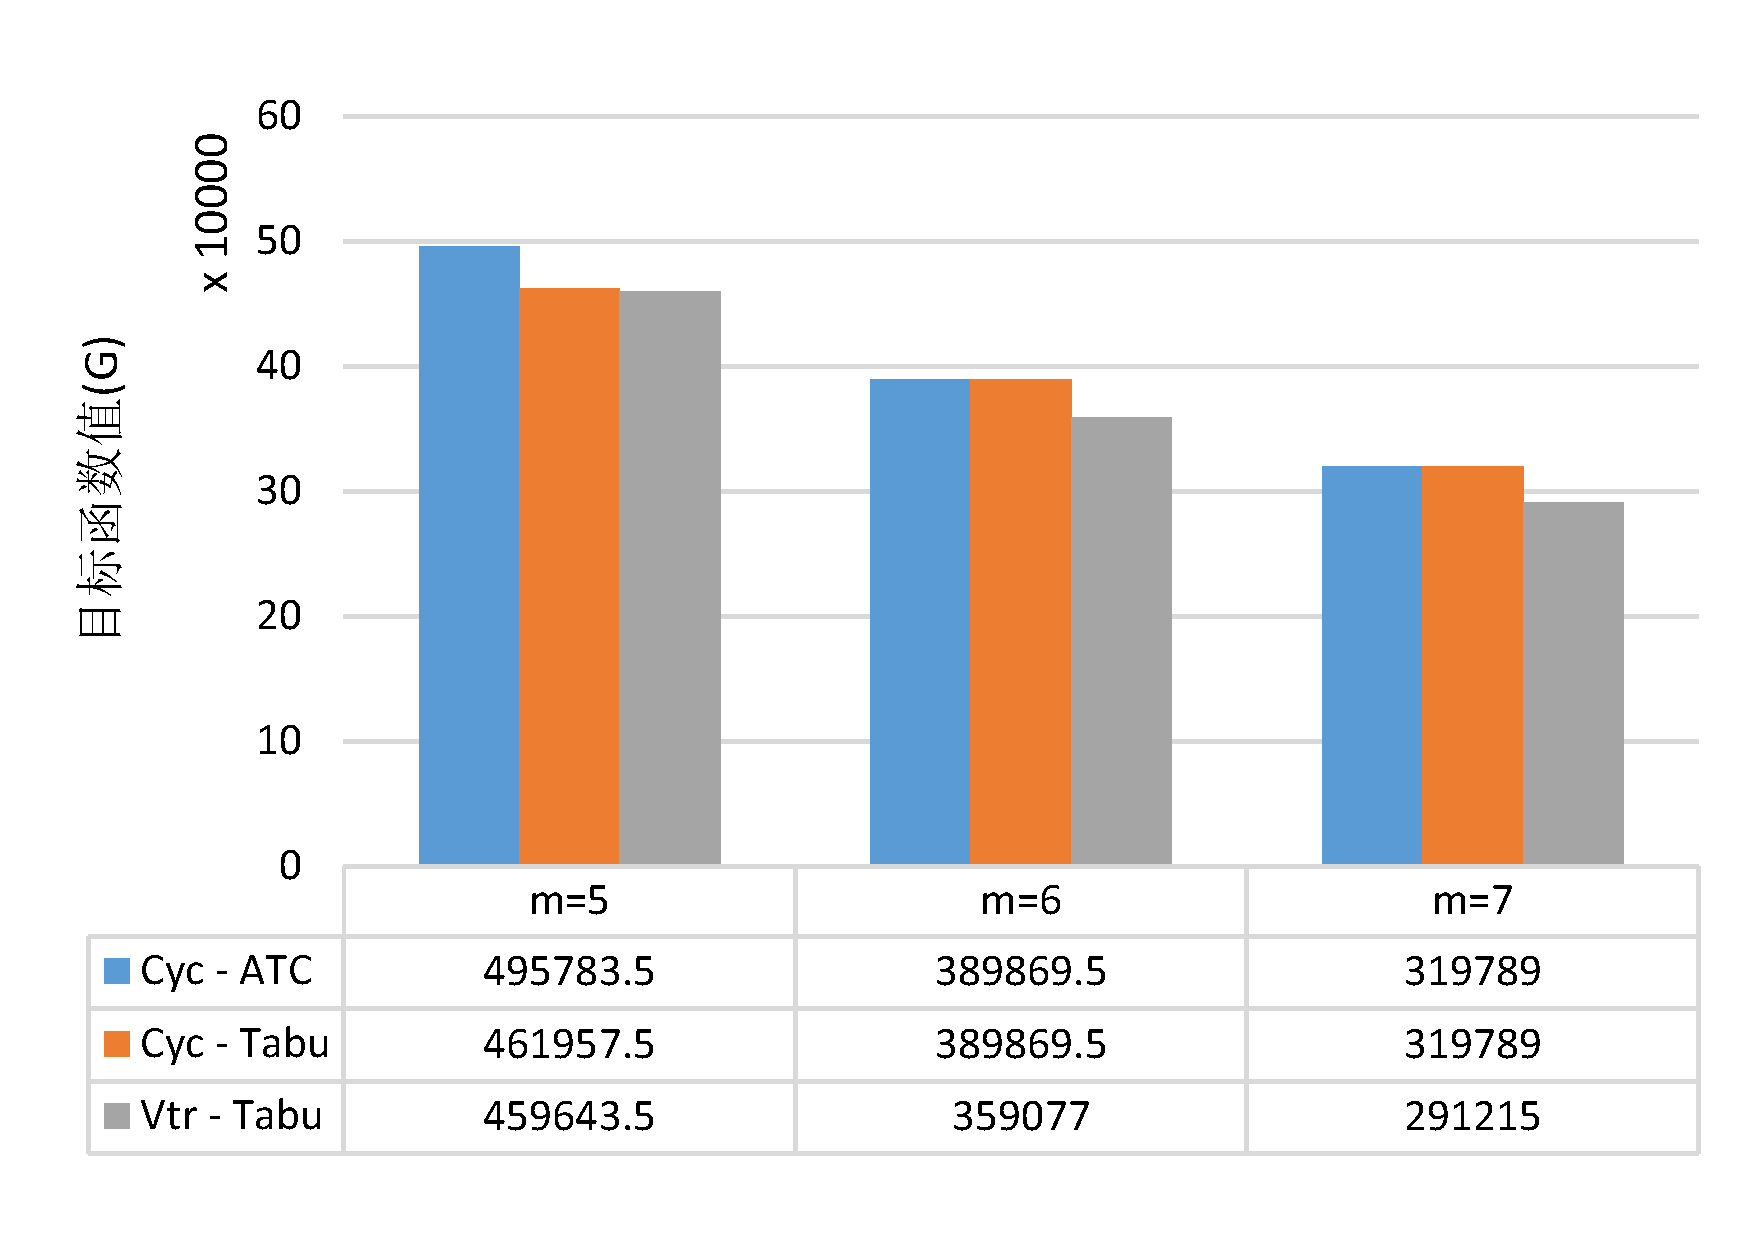
\includegraphics[height = 6cm, angle = -90]{basic_05_200}}
\subfloat[$n = 300$]{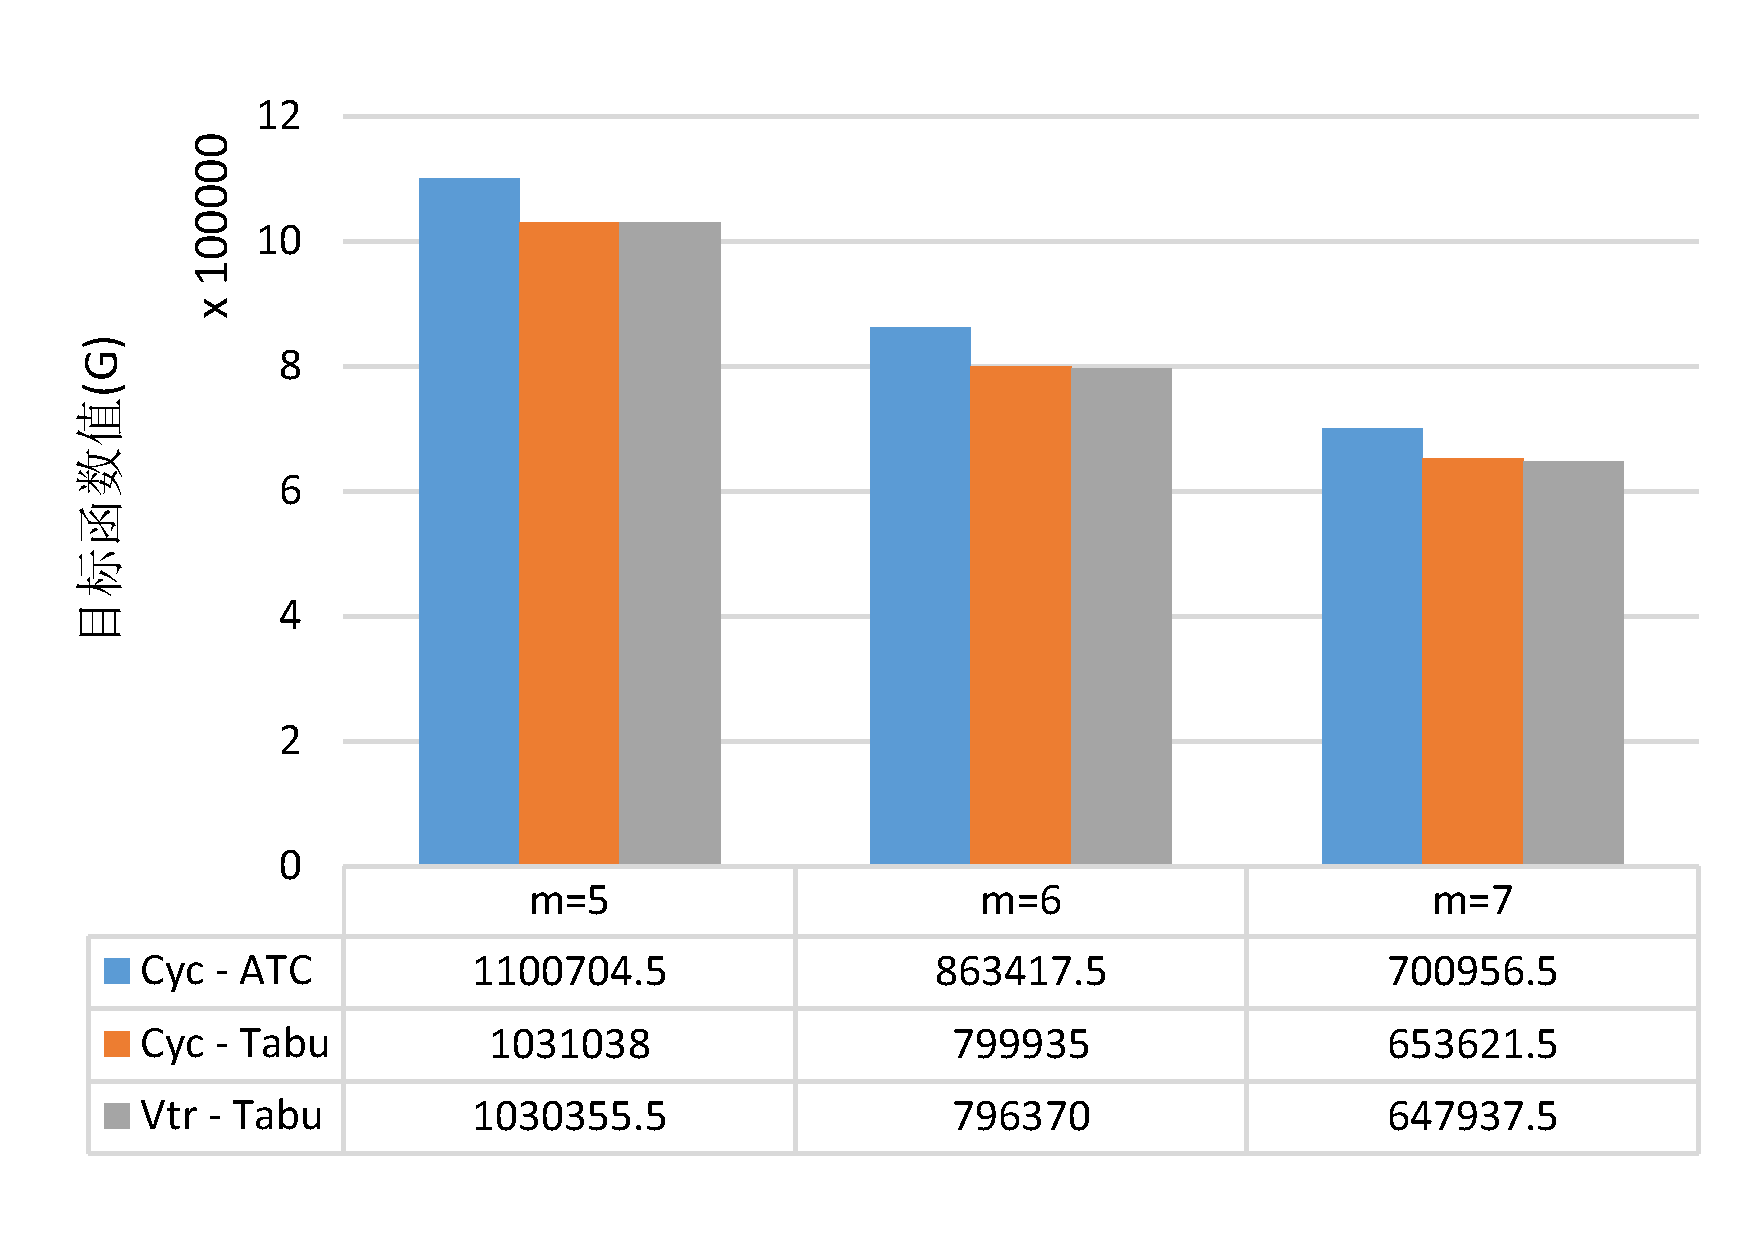
\includegraphics[height = 6cm, angle = -90]{basic_05_300}}\\
\subfloat[$n = 500$]{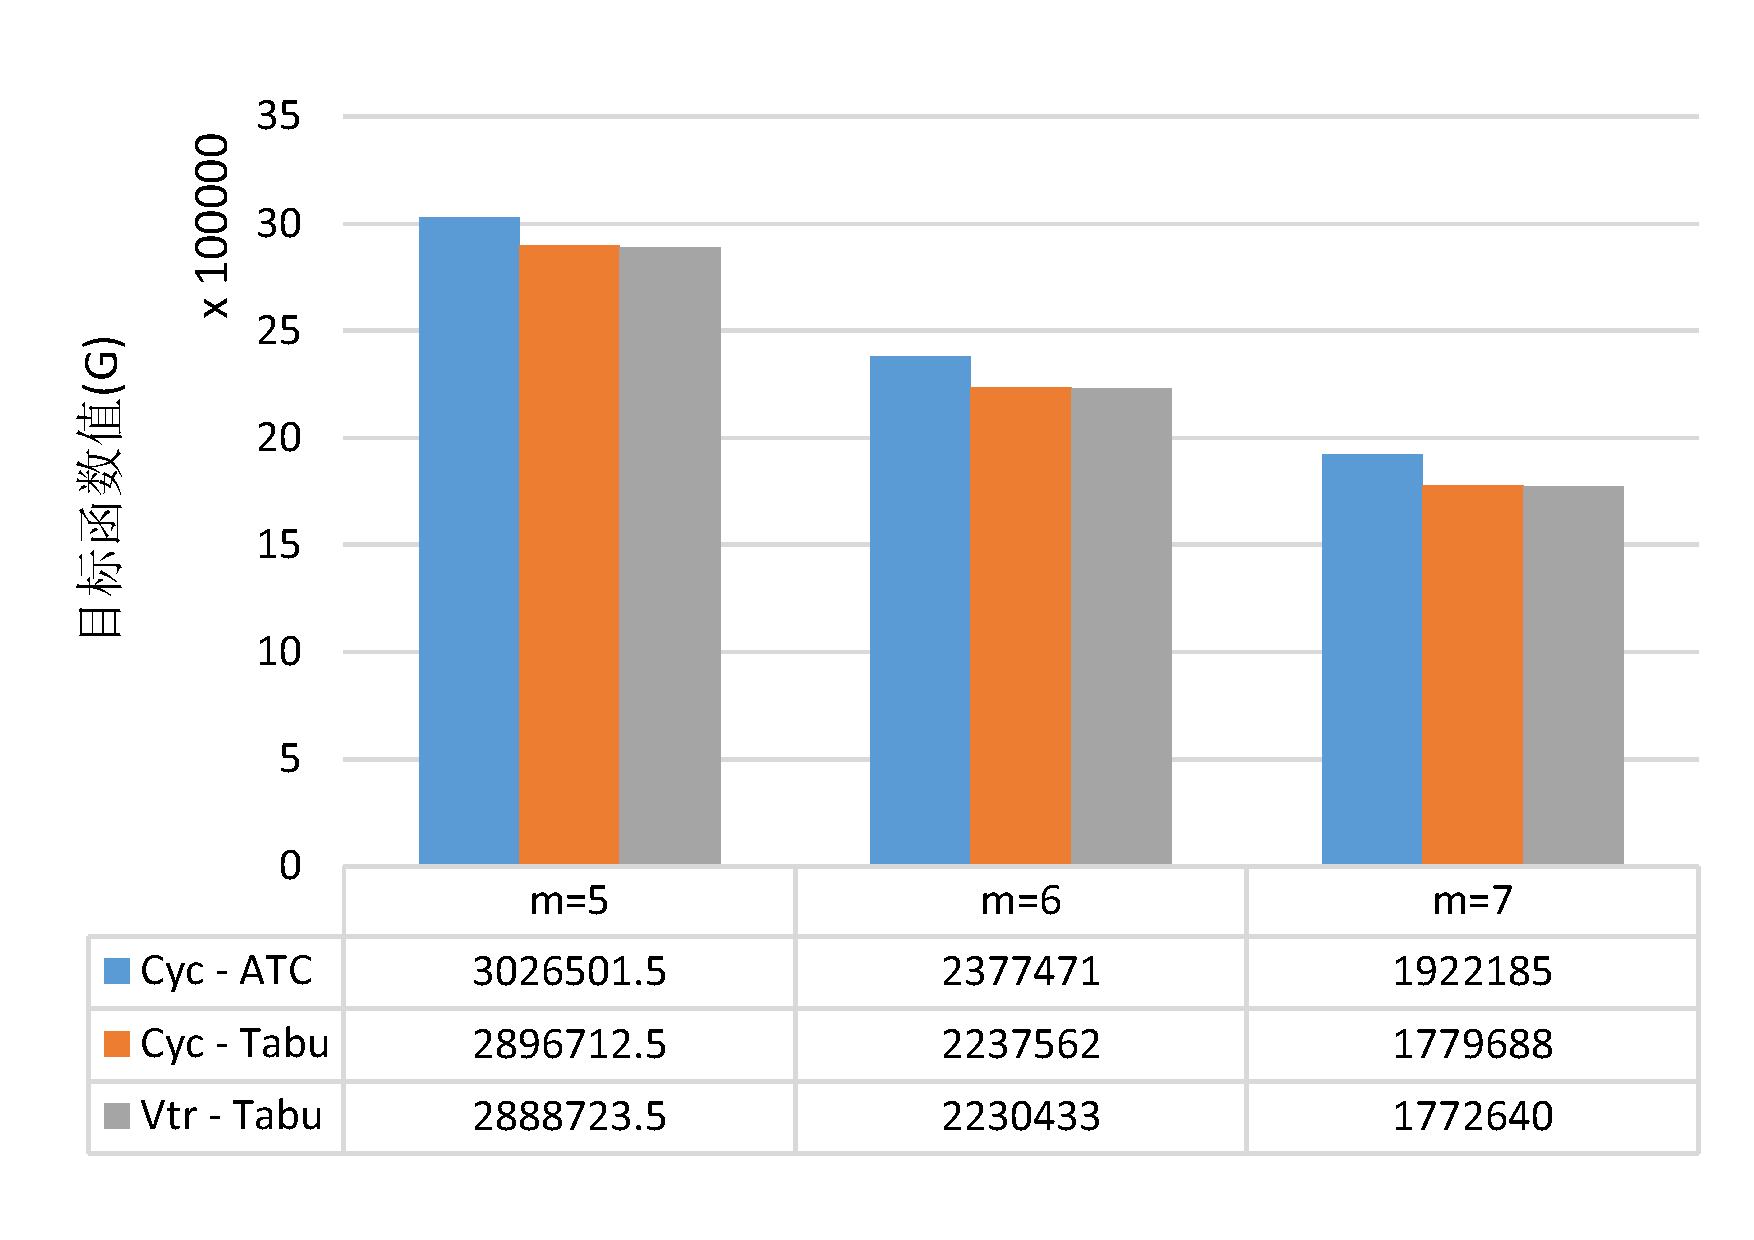
\includegraphics[height = 6cm, angle = -90]{basic_05_500}}
\subfloat[$n = 750$]{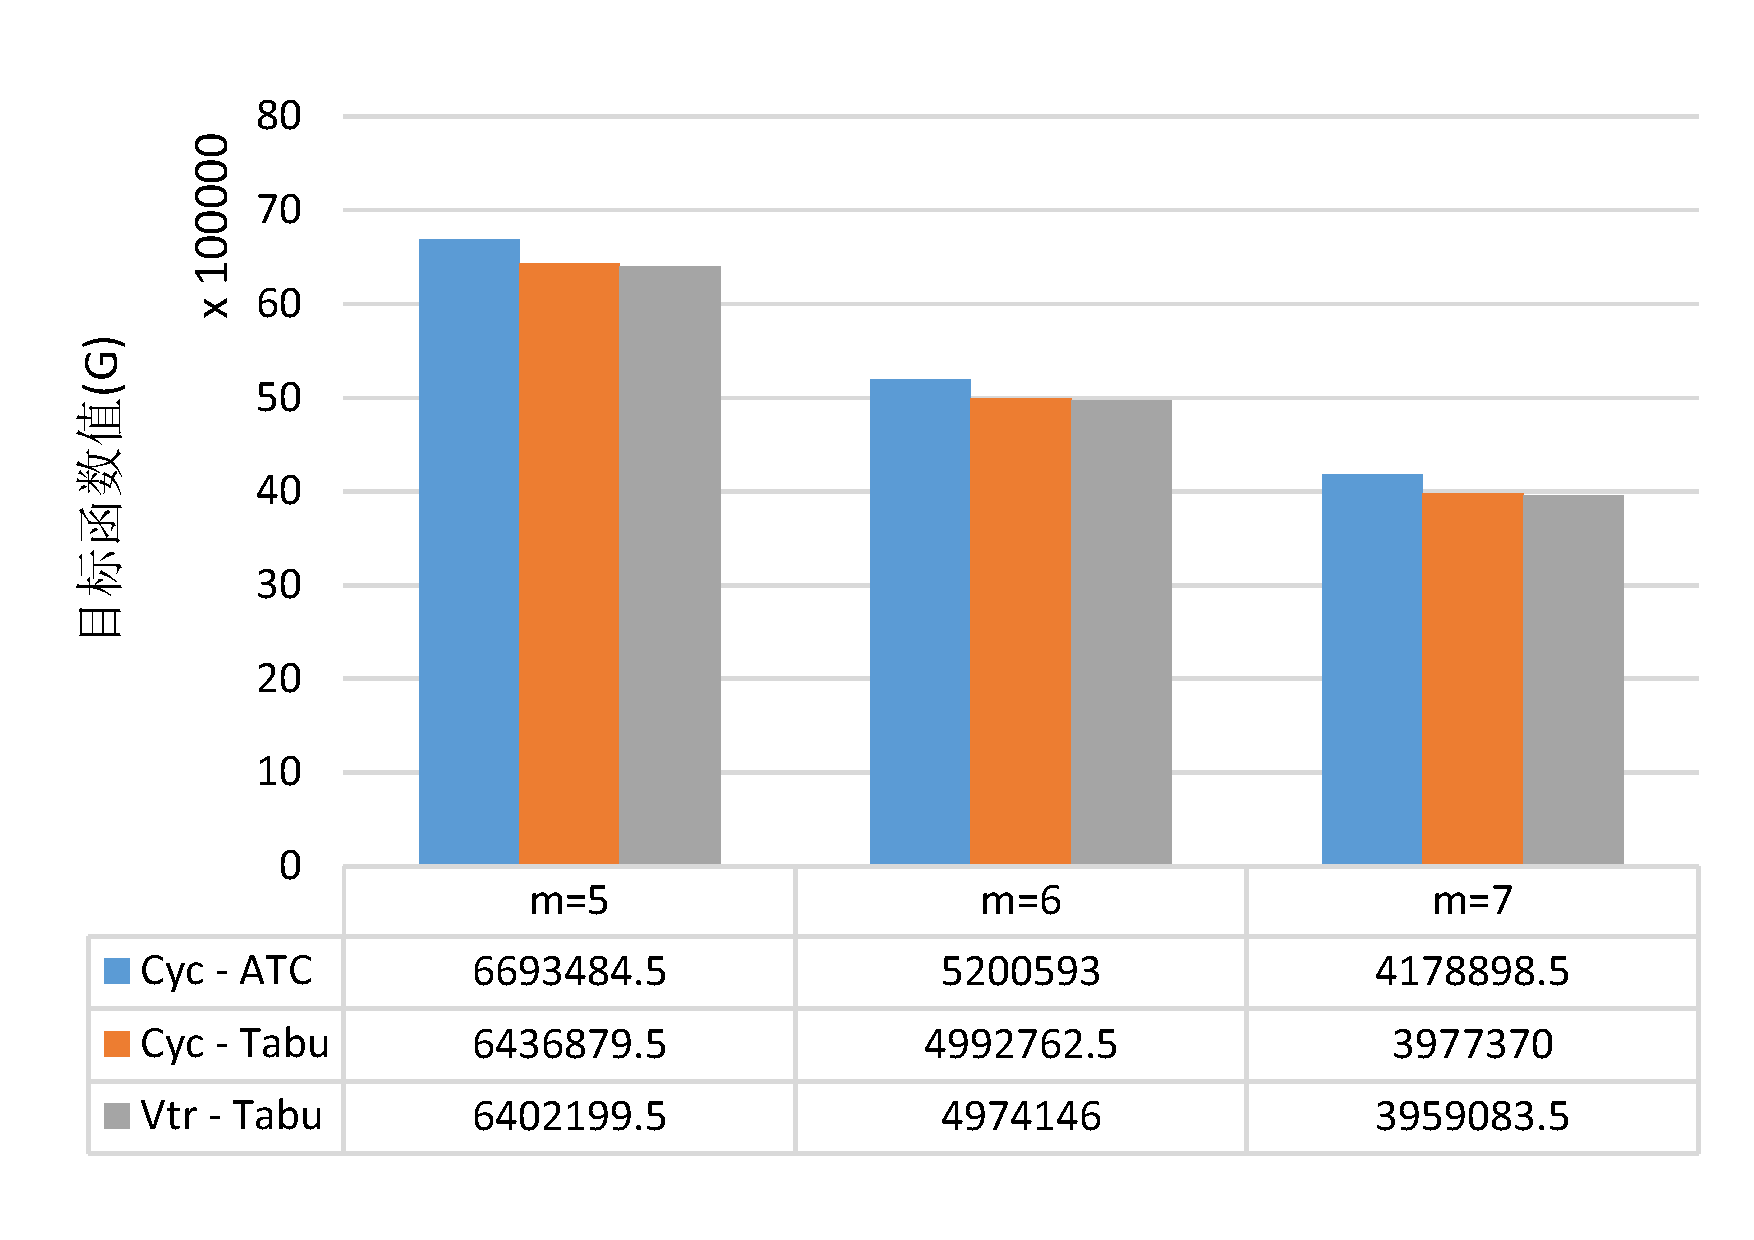
\includegraphics[height = 6cm, angle = -90]{basic_05_750}}
\subfloat[$n = 1000$]{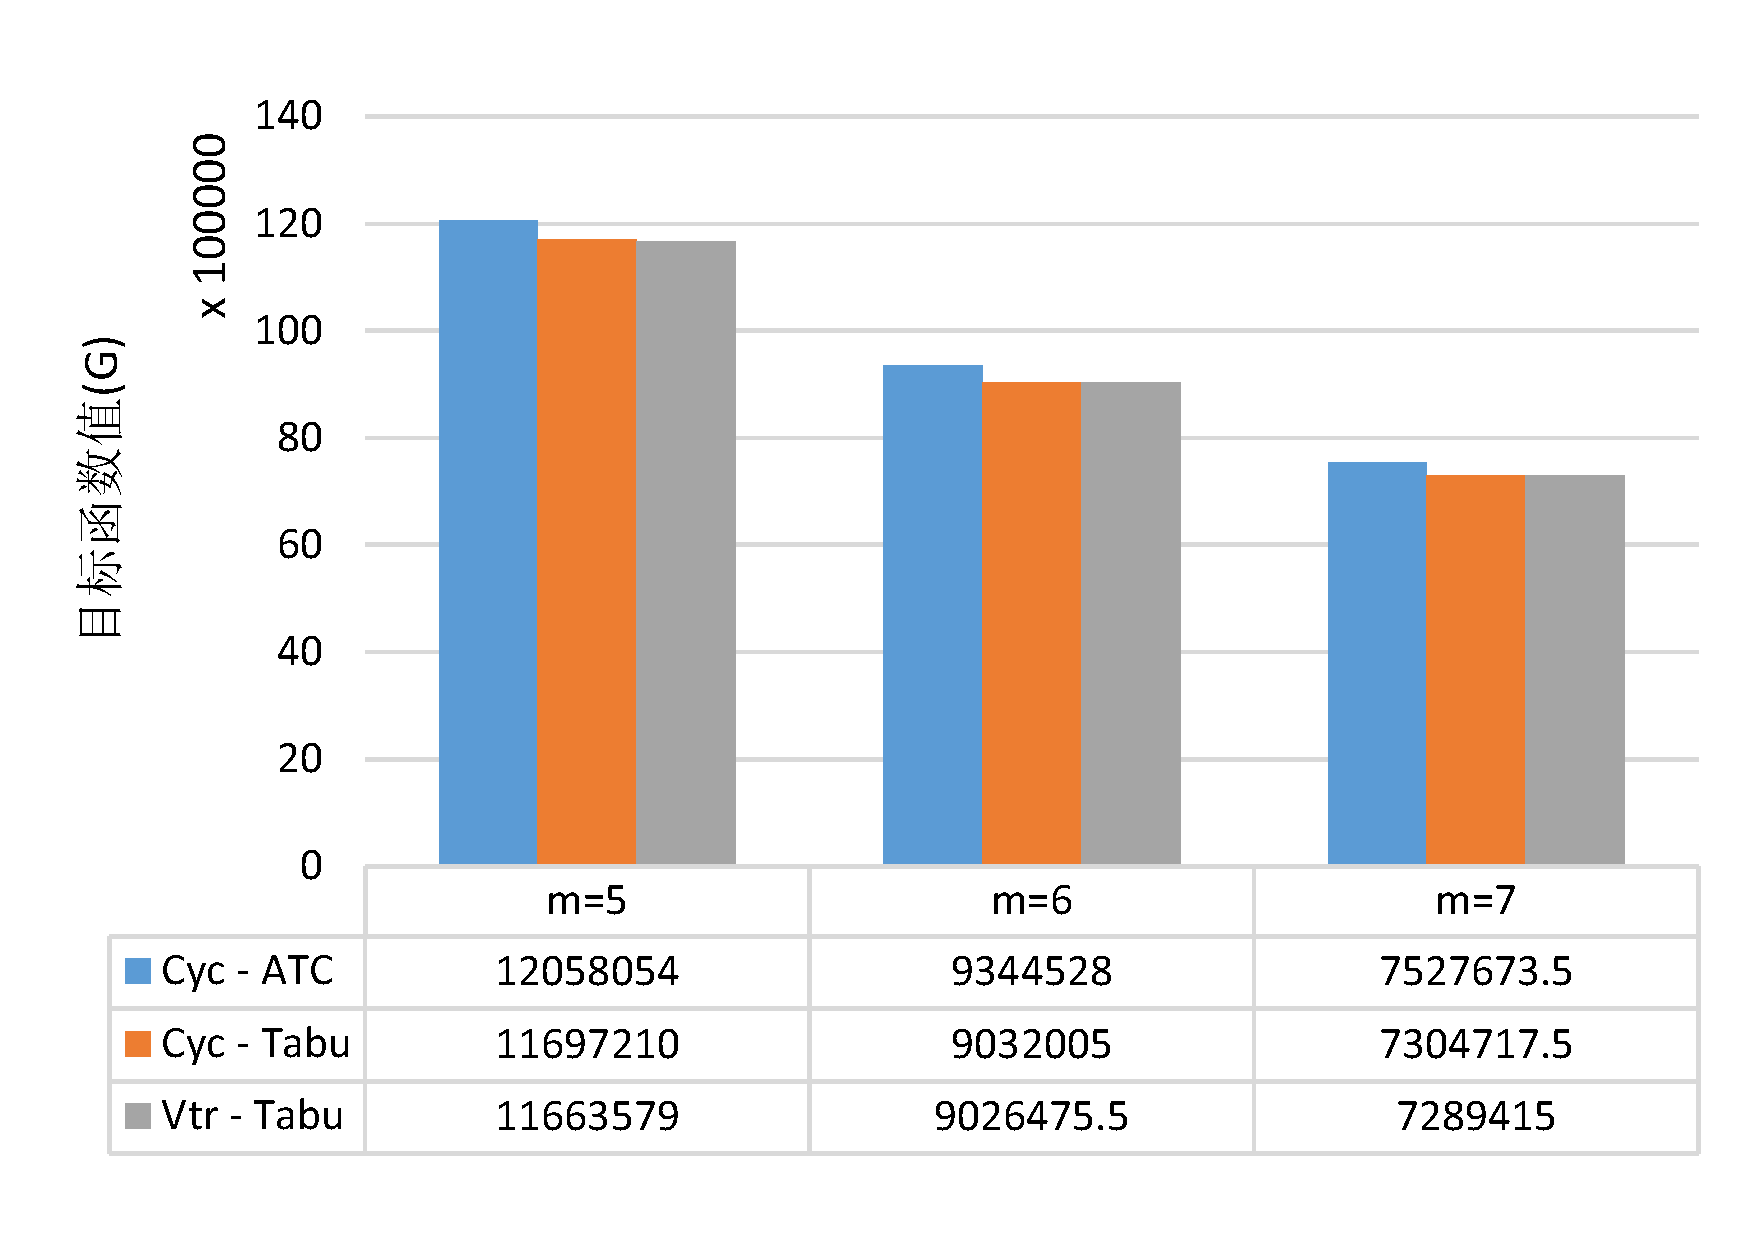
\includegraphics[height = 6cm, angle = -90]{basic_05_1000}}
\caption{\label{fig:result2}模型$1$的Cyc -- ATC、Cyc -- Tabu、Vtr -- Tabu 算法求解目标函数值比较$(\lambda_1 = 0.5)$}
\end{sidewaysfigure}

\begin{sidewaysfigure}
\centering
\subfloat[$n = 20$]{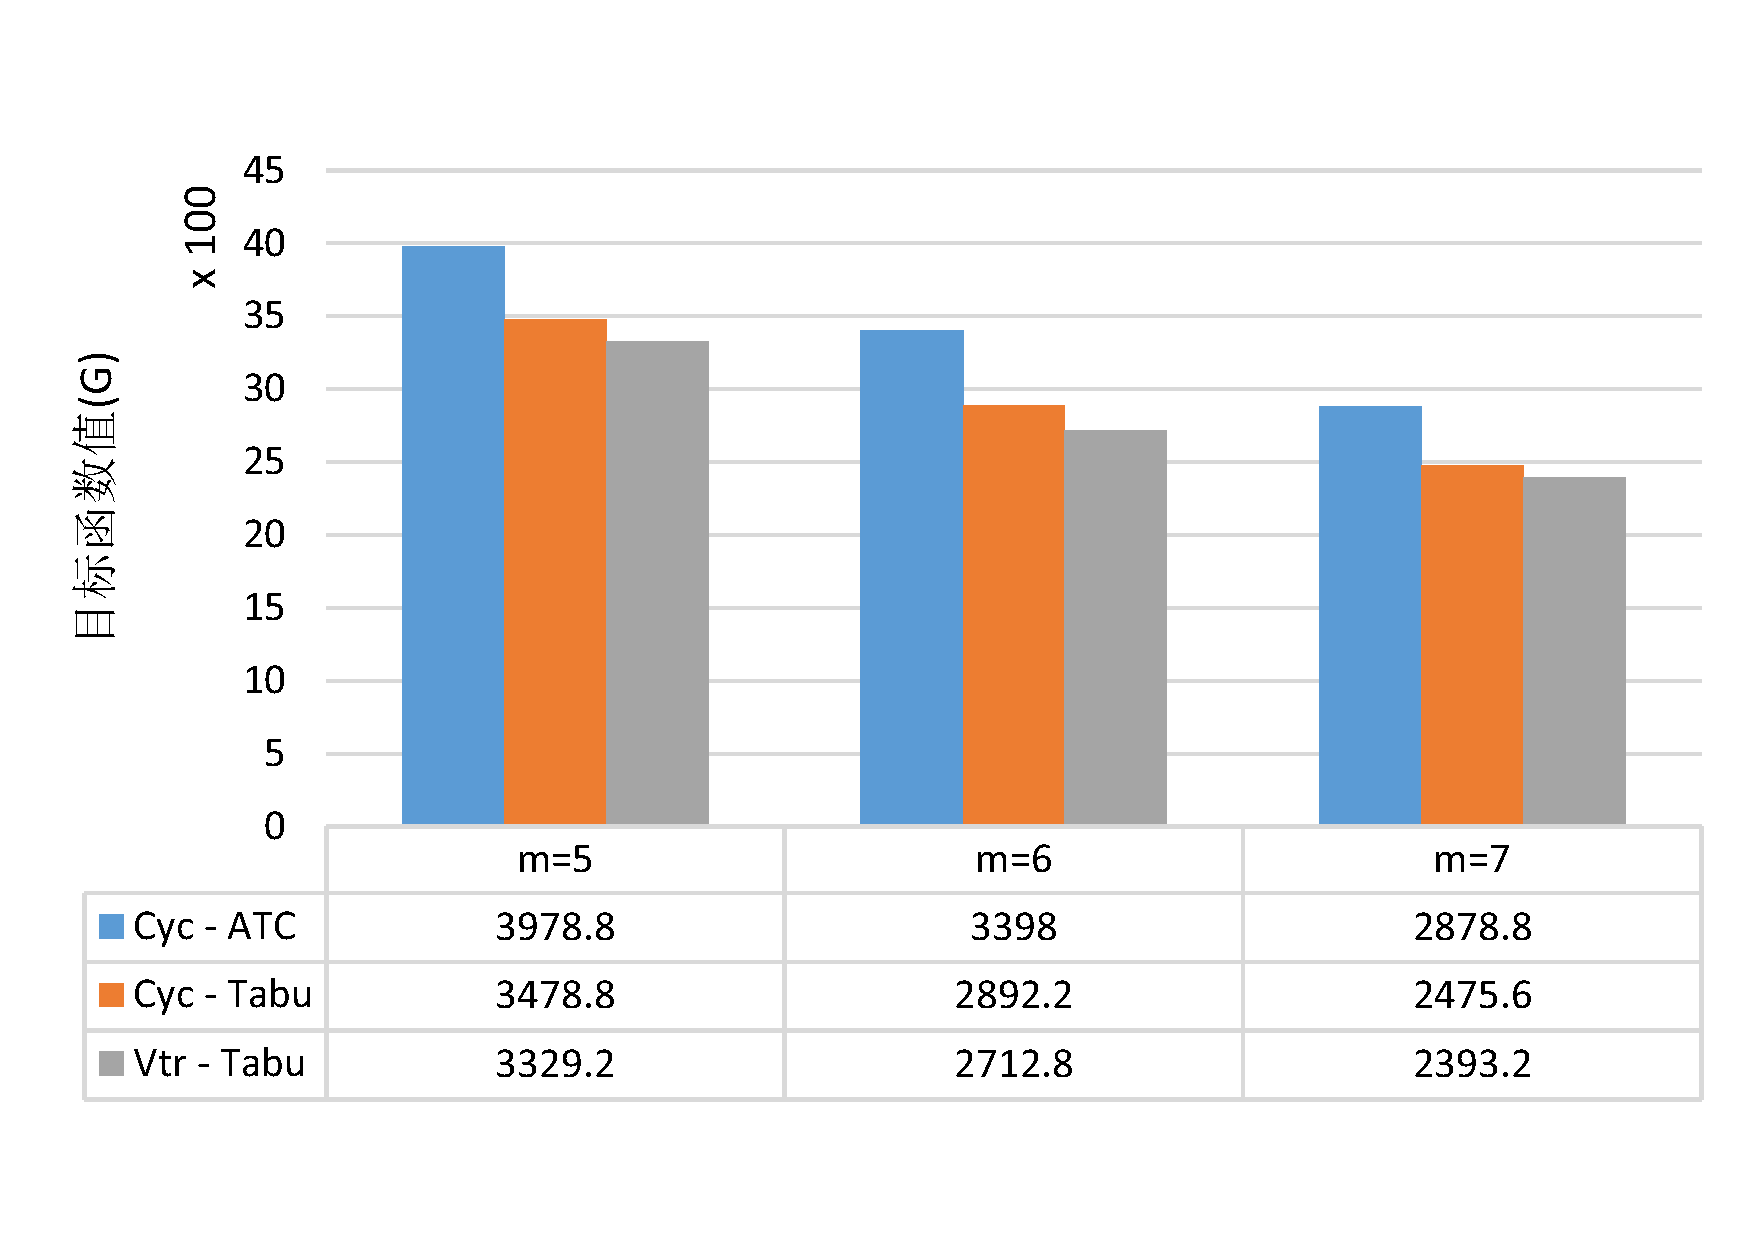
\includegraphics[height = 6cm, angle = -90]{basic_06_20}}
\subfloat[$n = 30$]{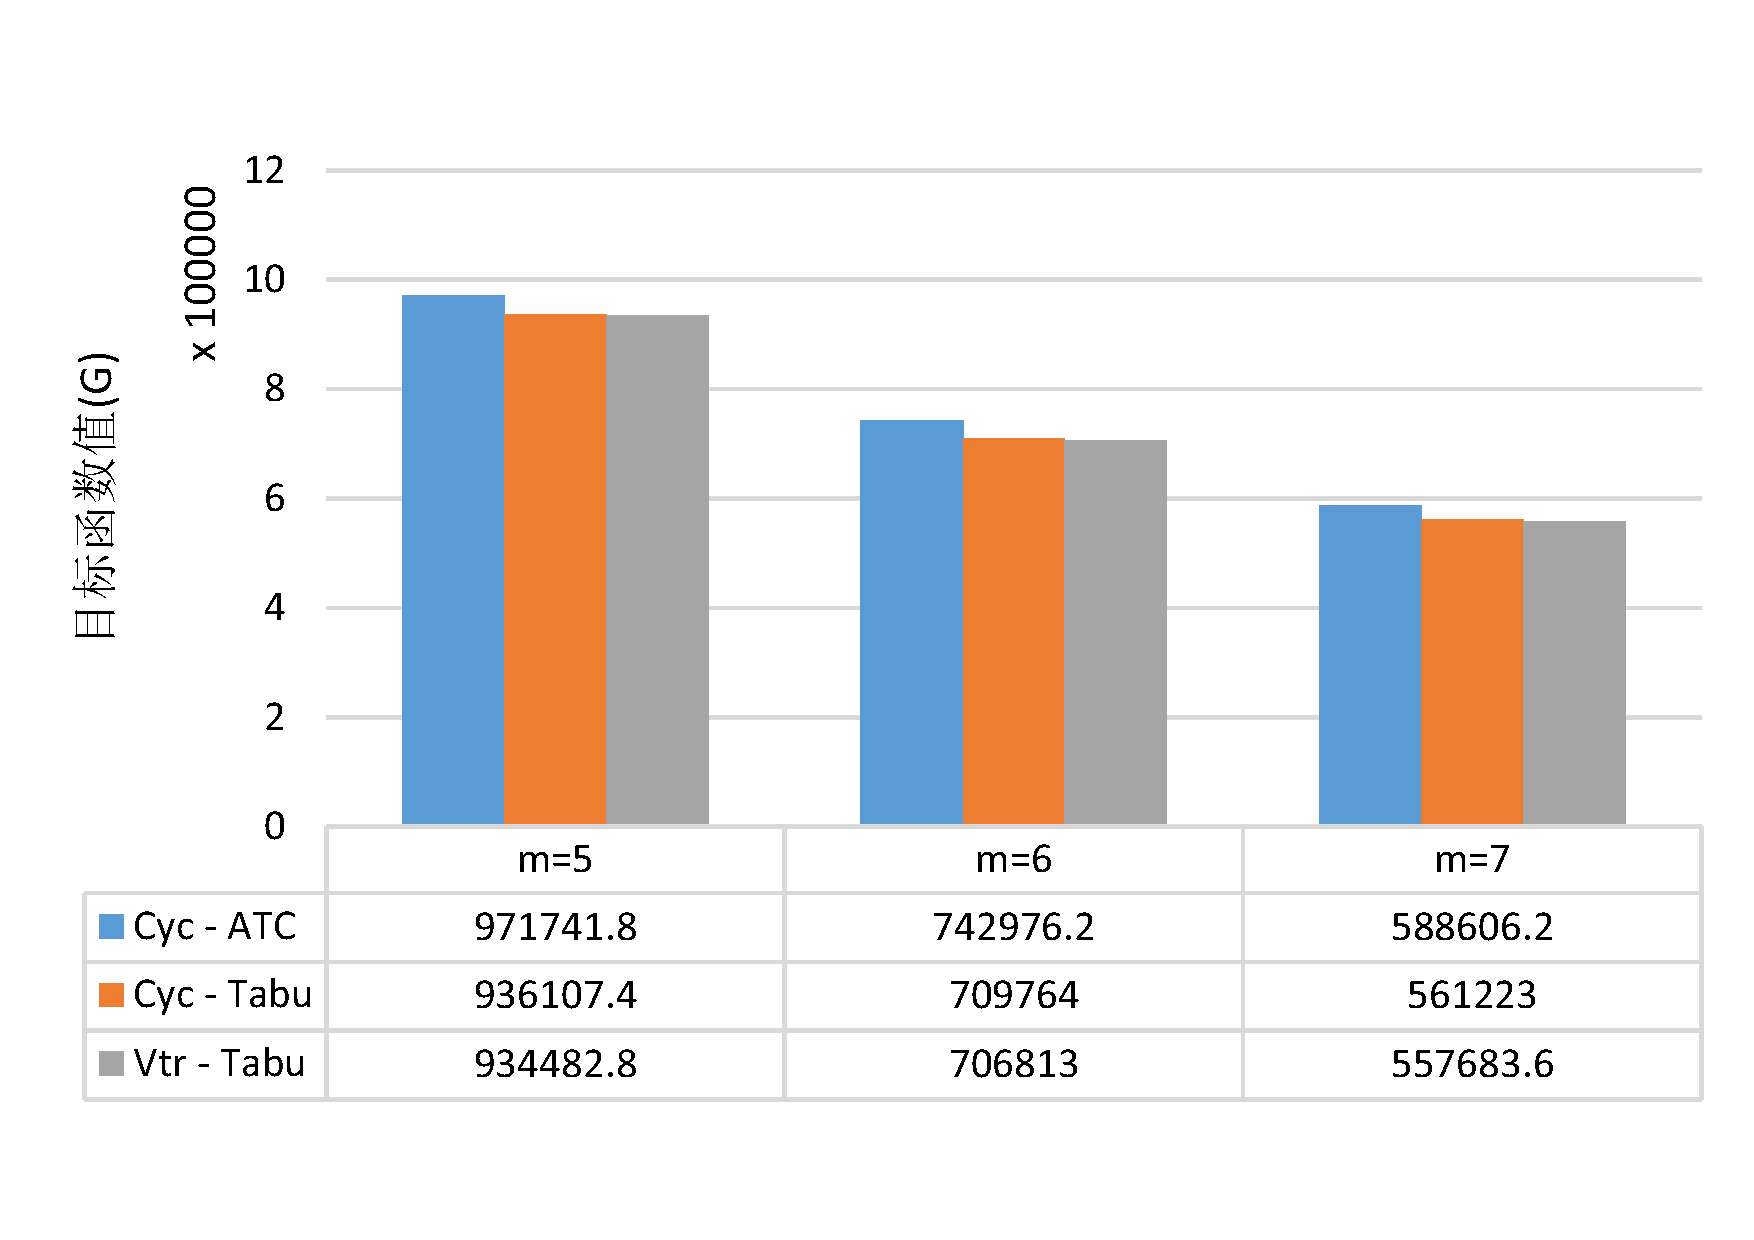
\includegraphics[height = 6cm, angle = -90]{basic_06_300}}
\subfloat[$n = 50$]{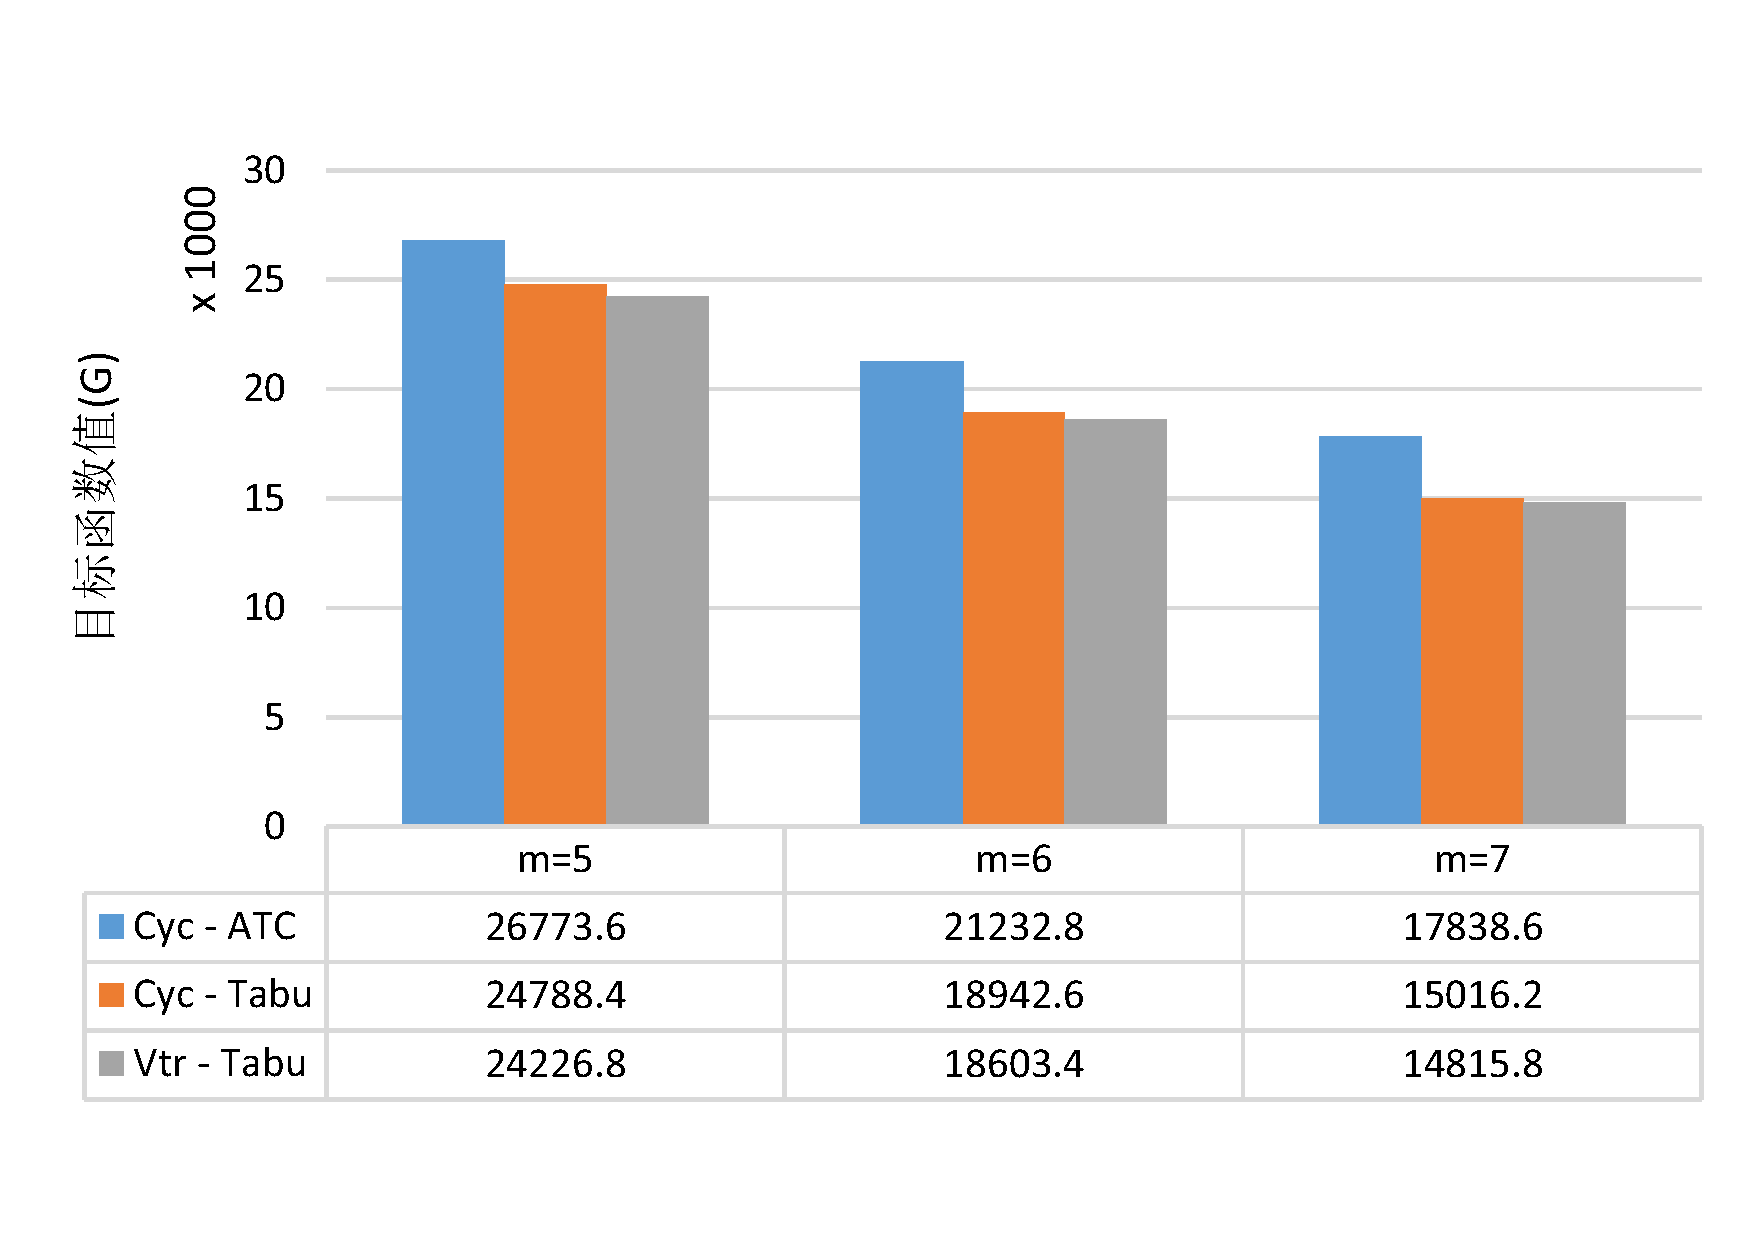
\includegraphics[height = 6cm, angle = -90]{basic_06_50}}
\subfloat[$n = 70$]{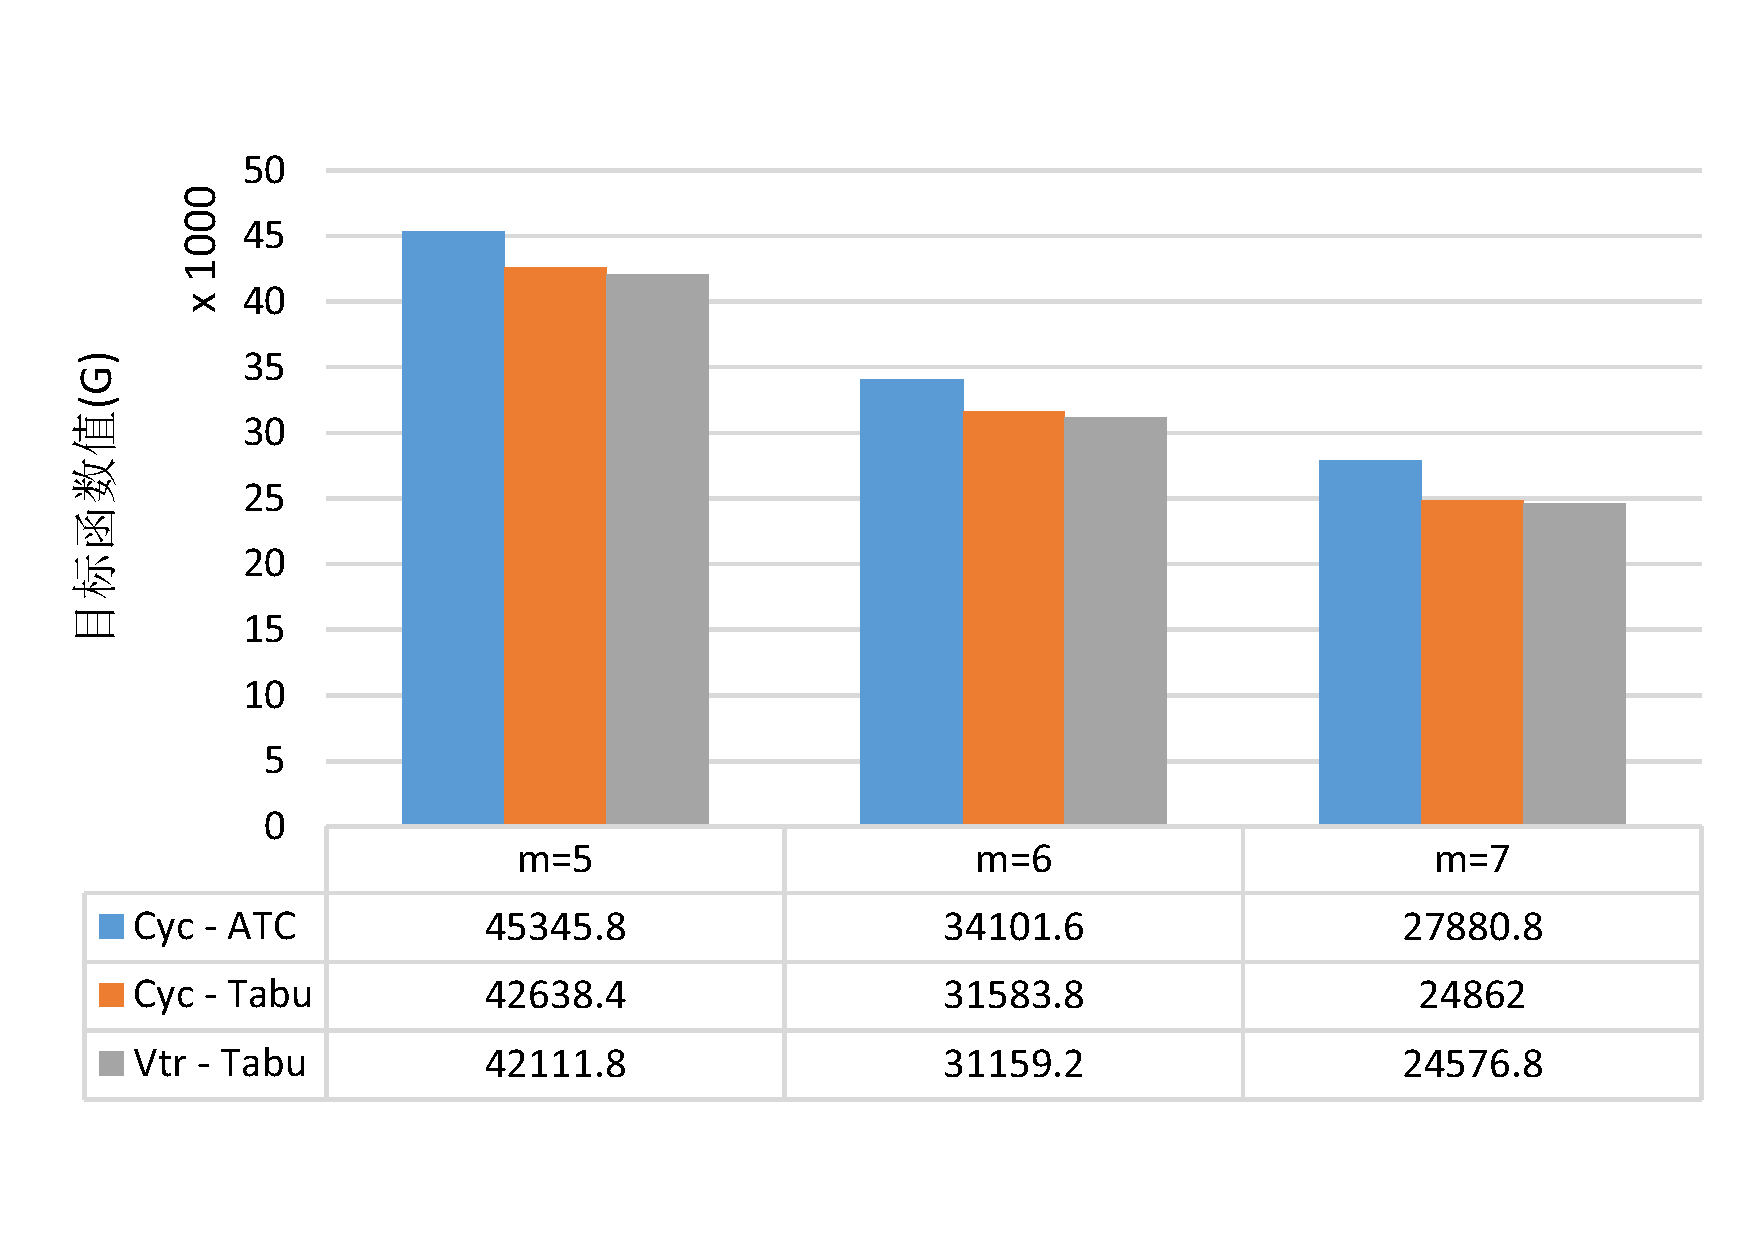
\includegraphics[height = 6cm, angle = -90]{basic_06_70}}\\
\subfloat[$n = 100$]{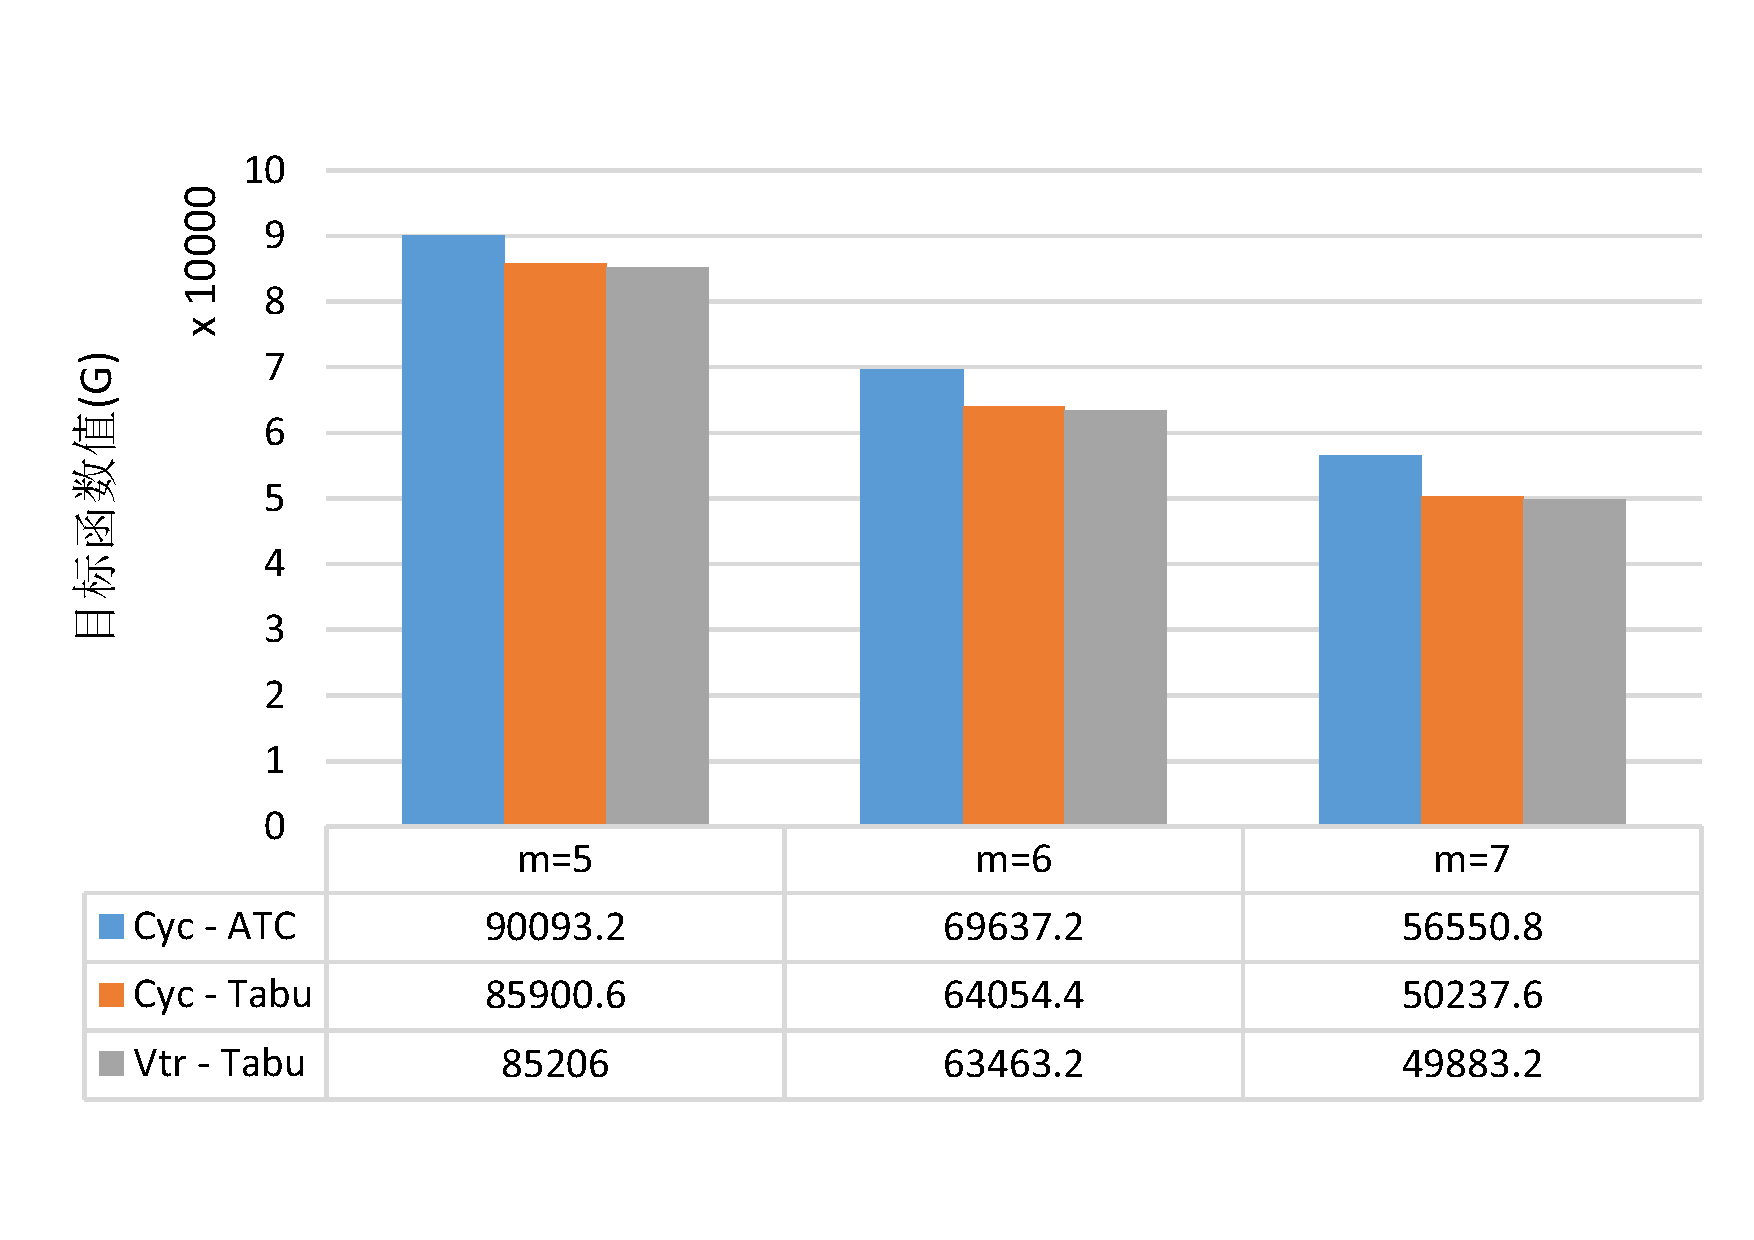
\includegraphics[height = 6cm, angle = -90]{basic_06_100}}
\subfloat[$n = 150$]{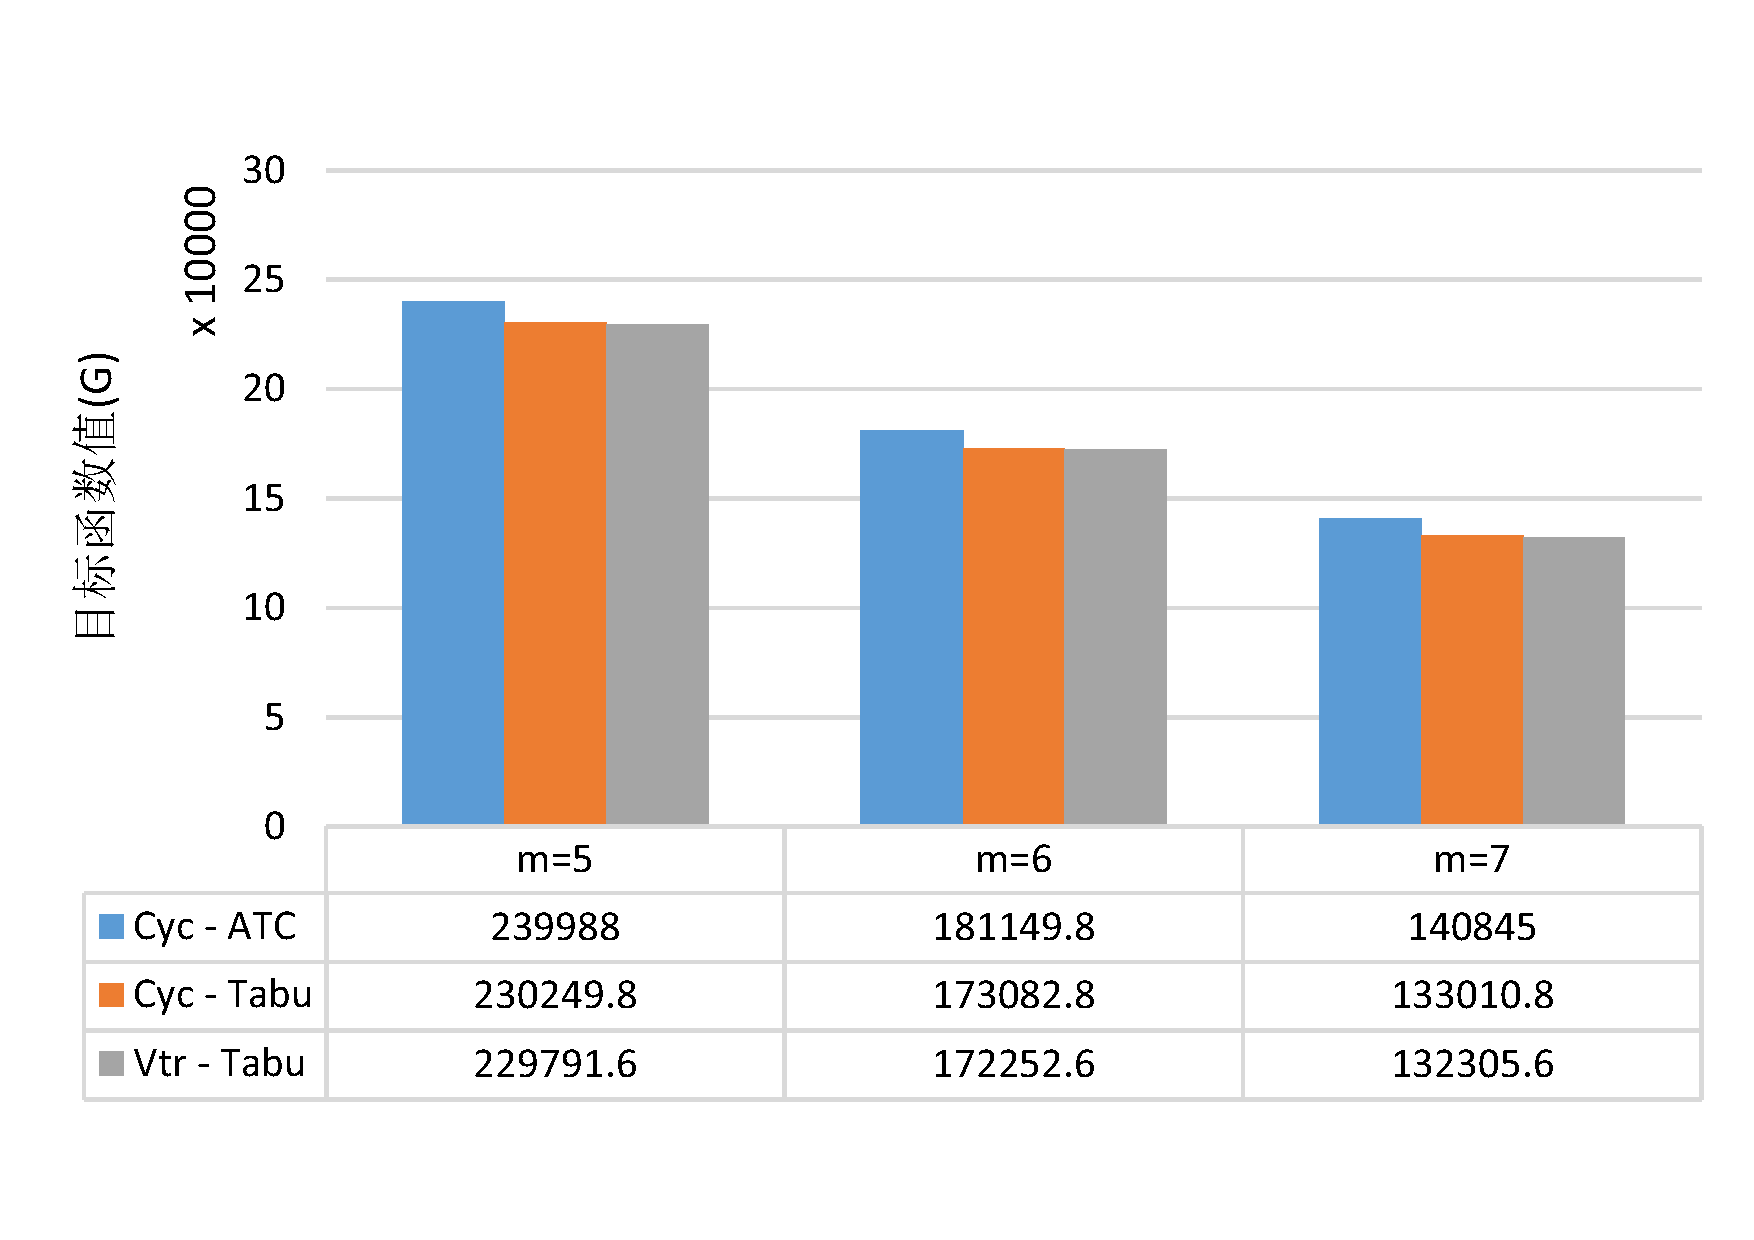
\includegraphics[height = 6cm, angle = -90]{basic_06_150}}
\subfloat[$n = 200$]{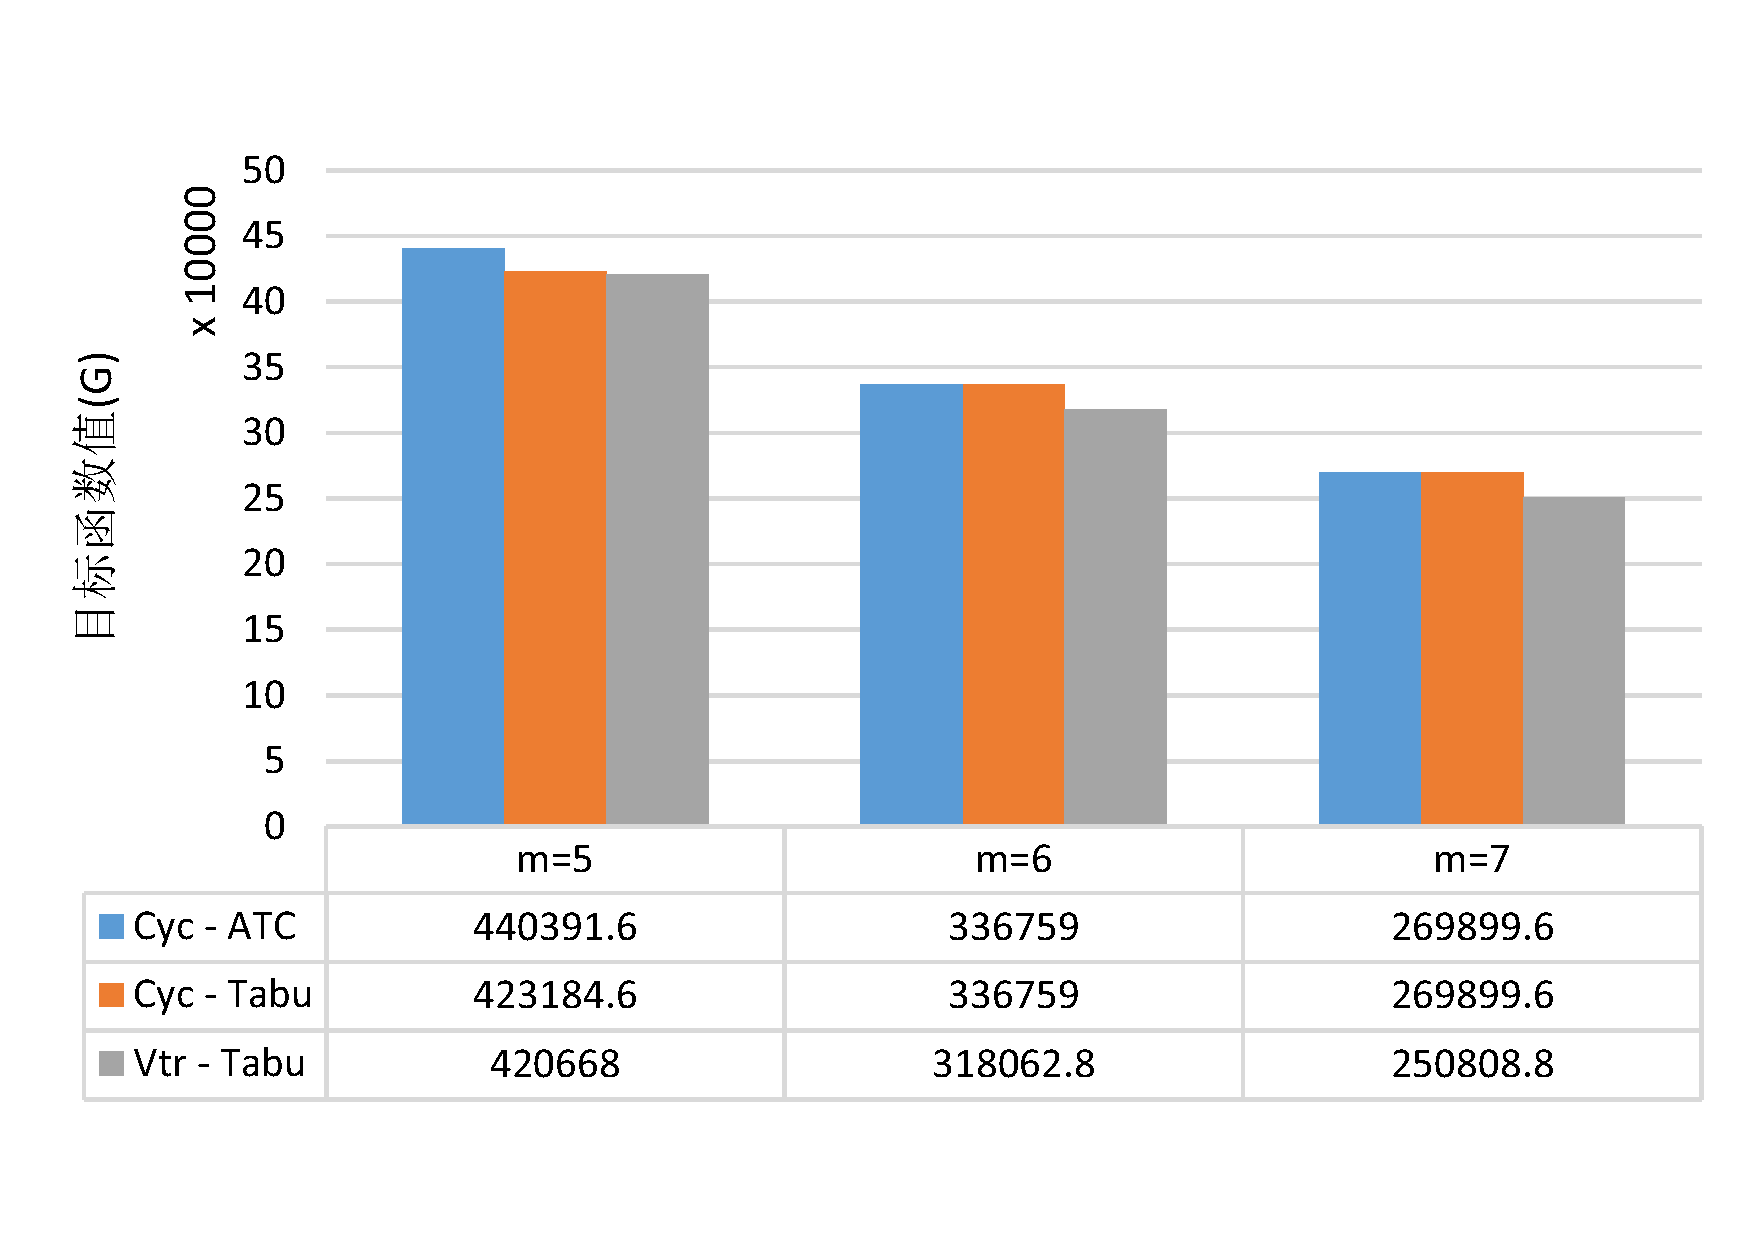
\includegraphics[height = 6cm, angle = -90]{basic_06_200}}
\subfloat[$n = 300$]{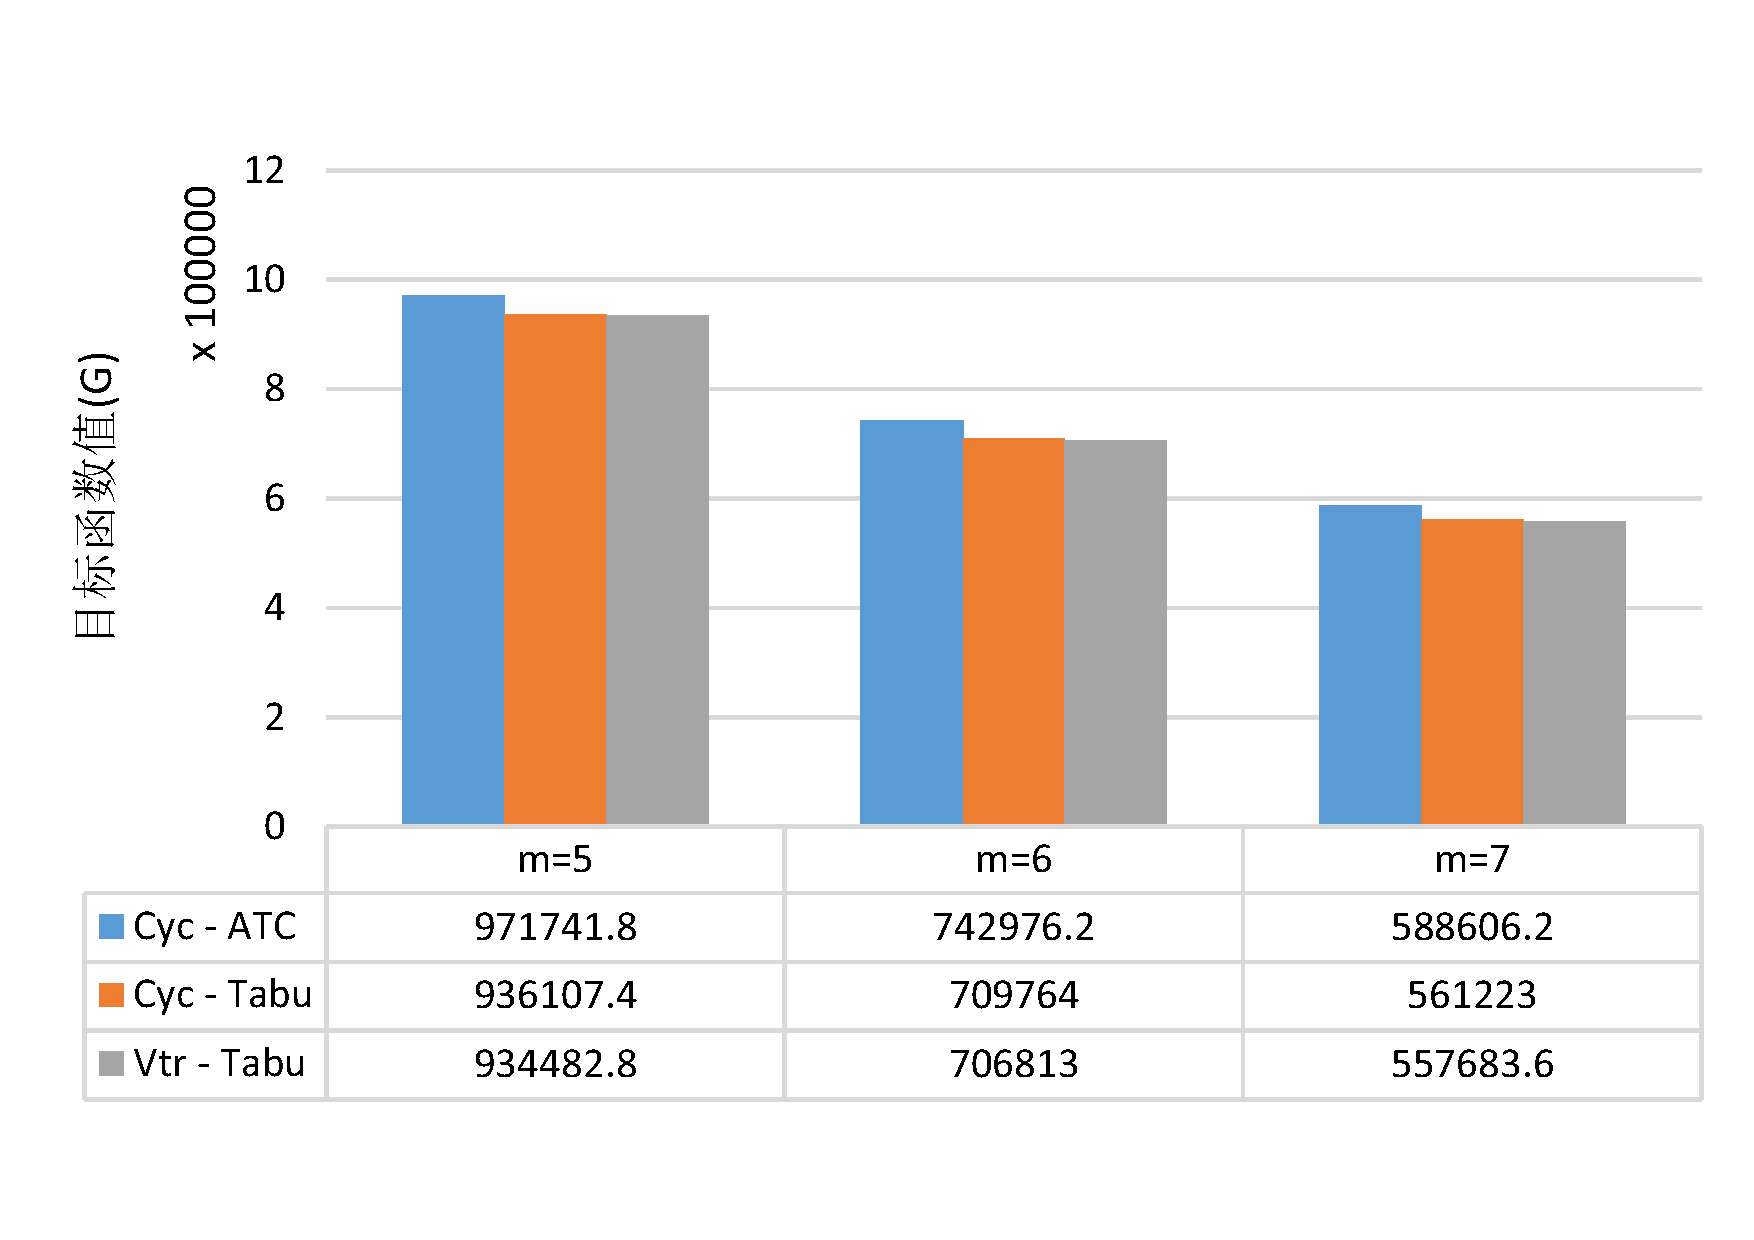
\includegraphics[height = 6cm, angle = -90]{basic_06_300}}\\
\subfloat[$n = 500$]{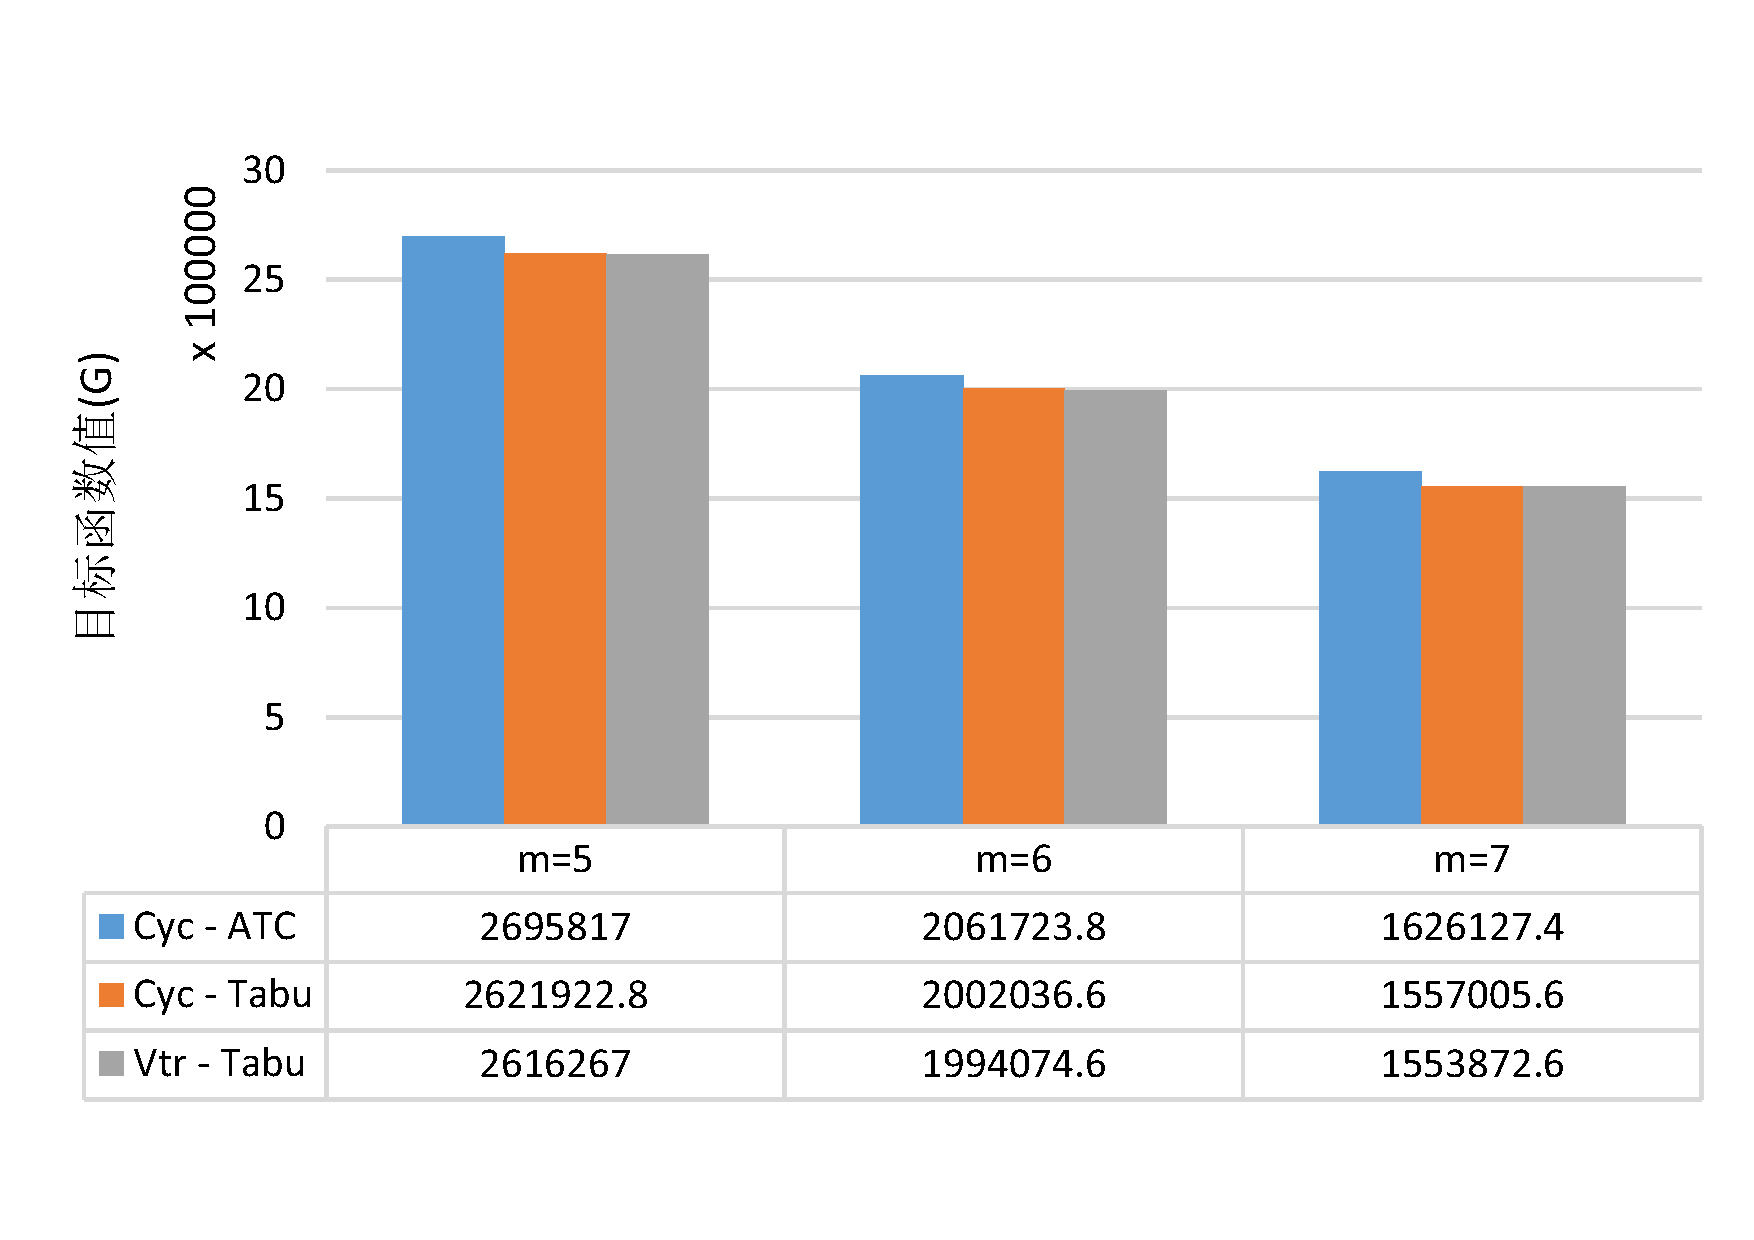
\includegraphics[height = 6cm, angle = -90]{basic_06_500}}
\subfloat[$n = 750$]{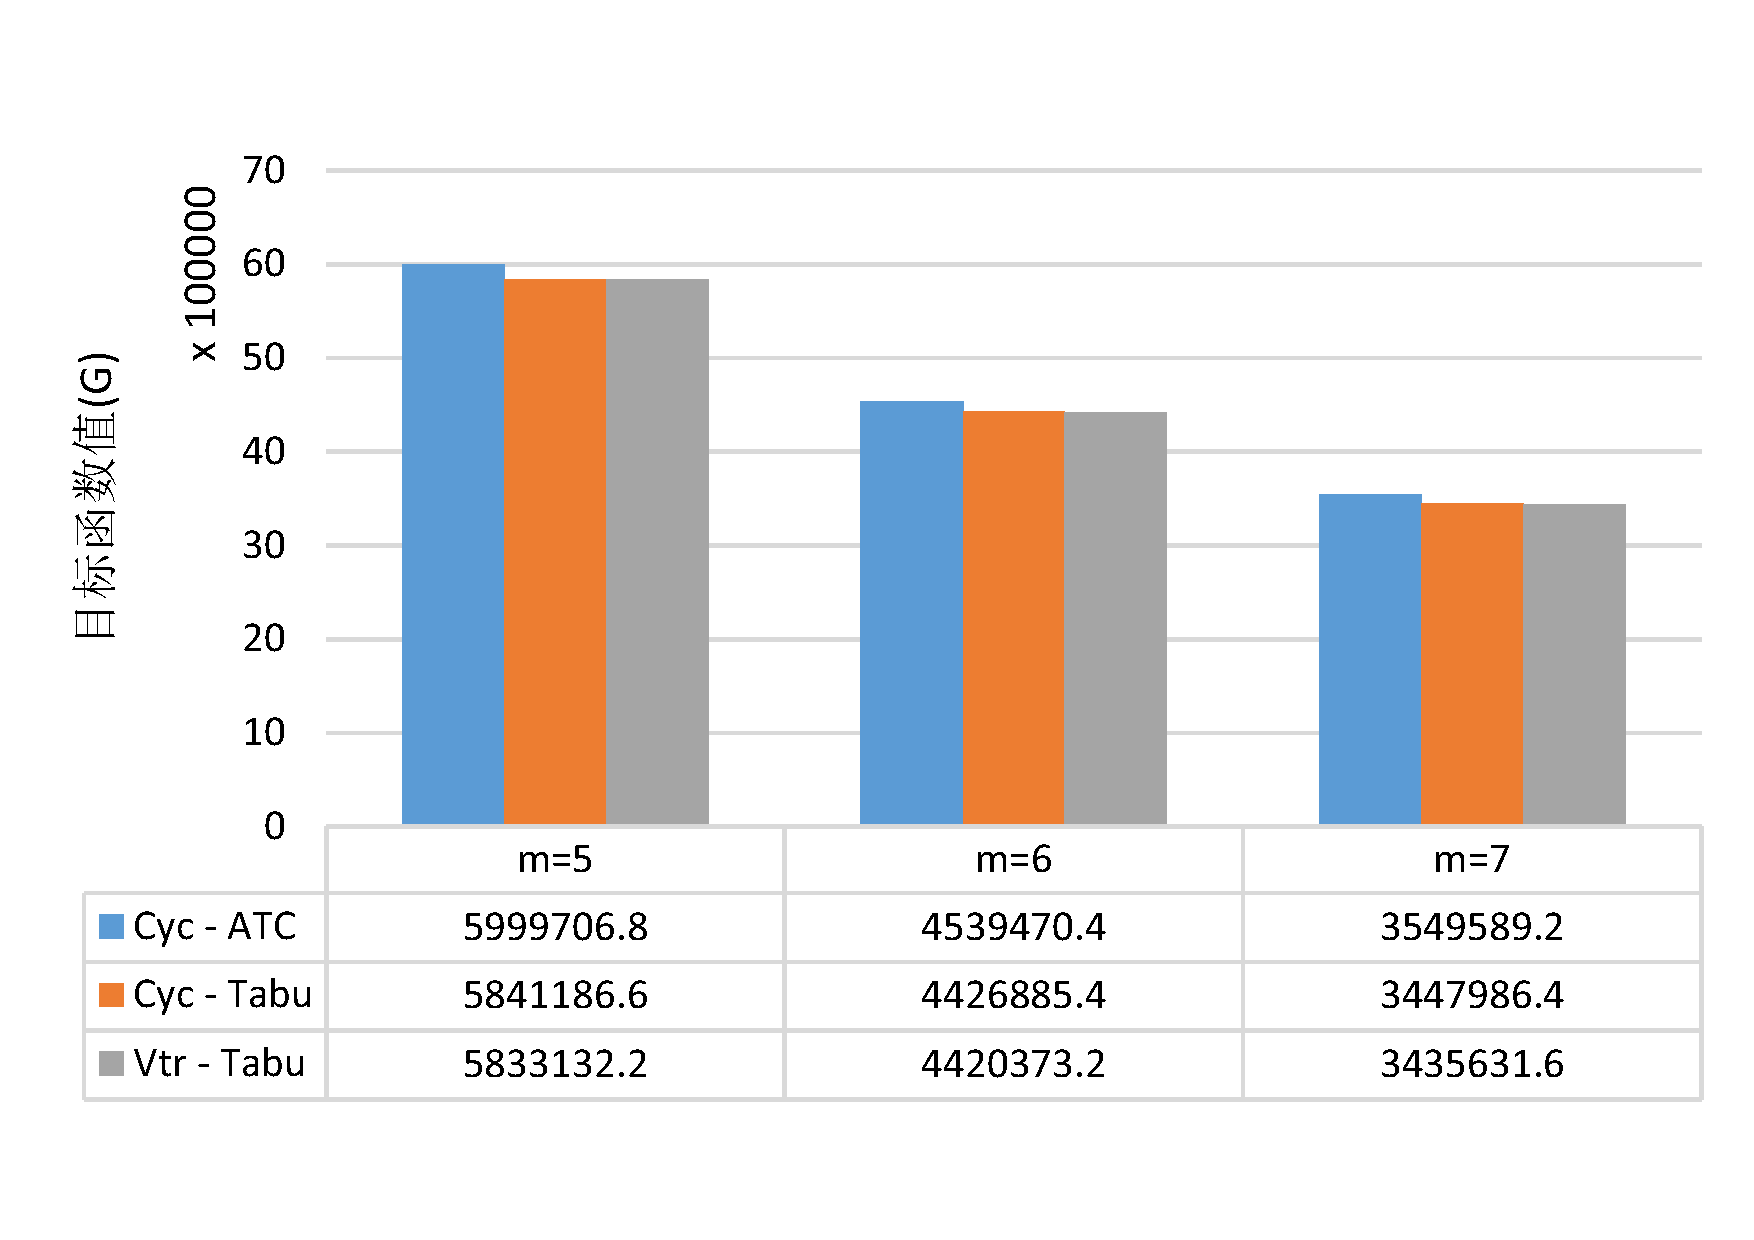
\includegraphics[height = 6cm, angle = -90]{basic_06_750}}
\subfloat[$n = 1000$]{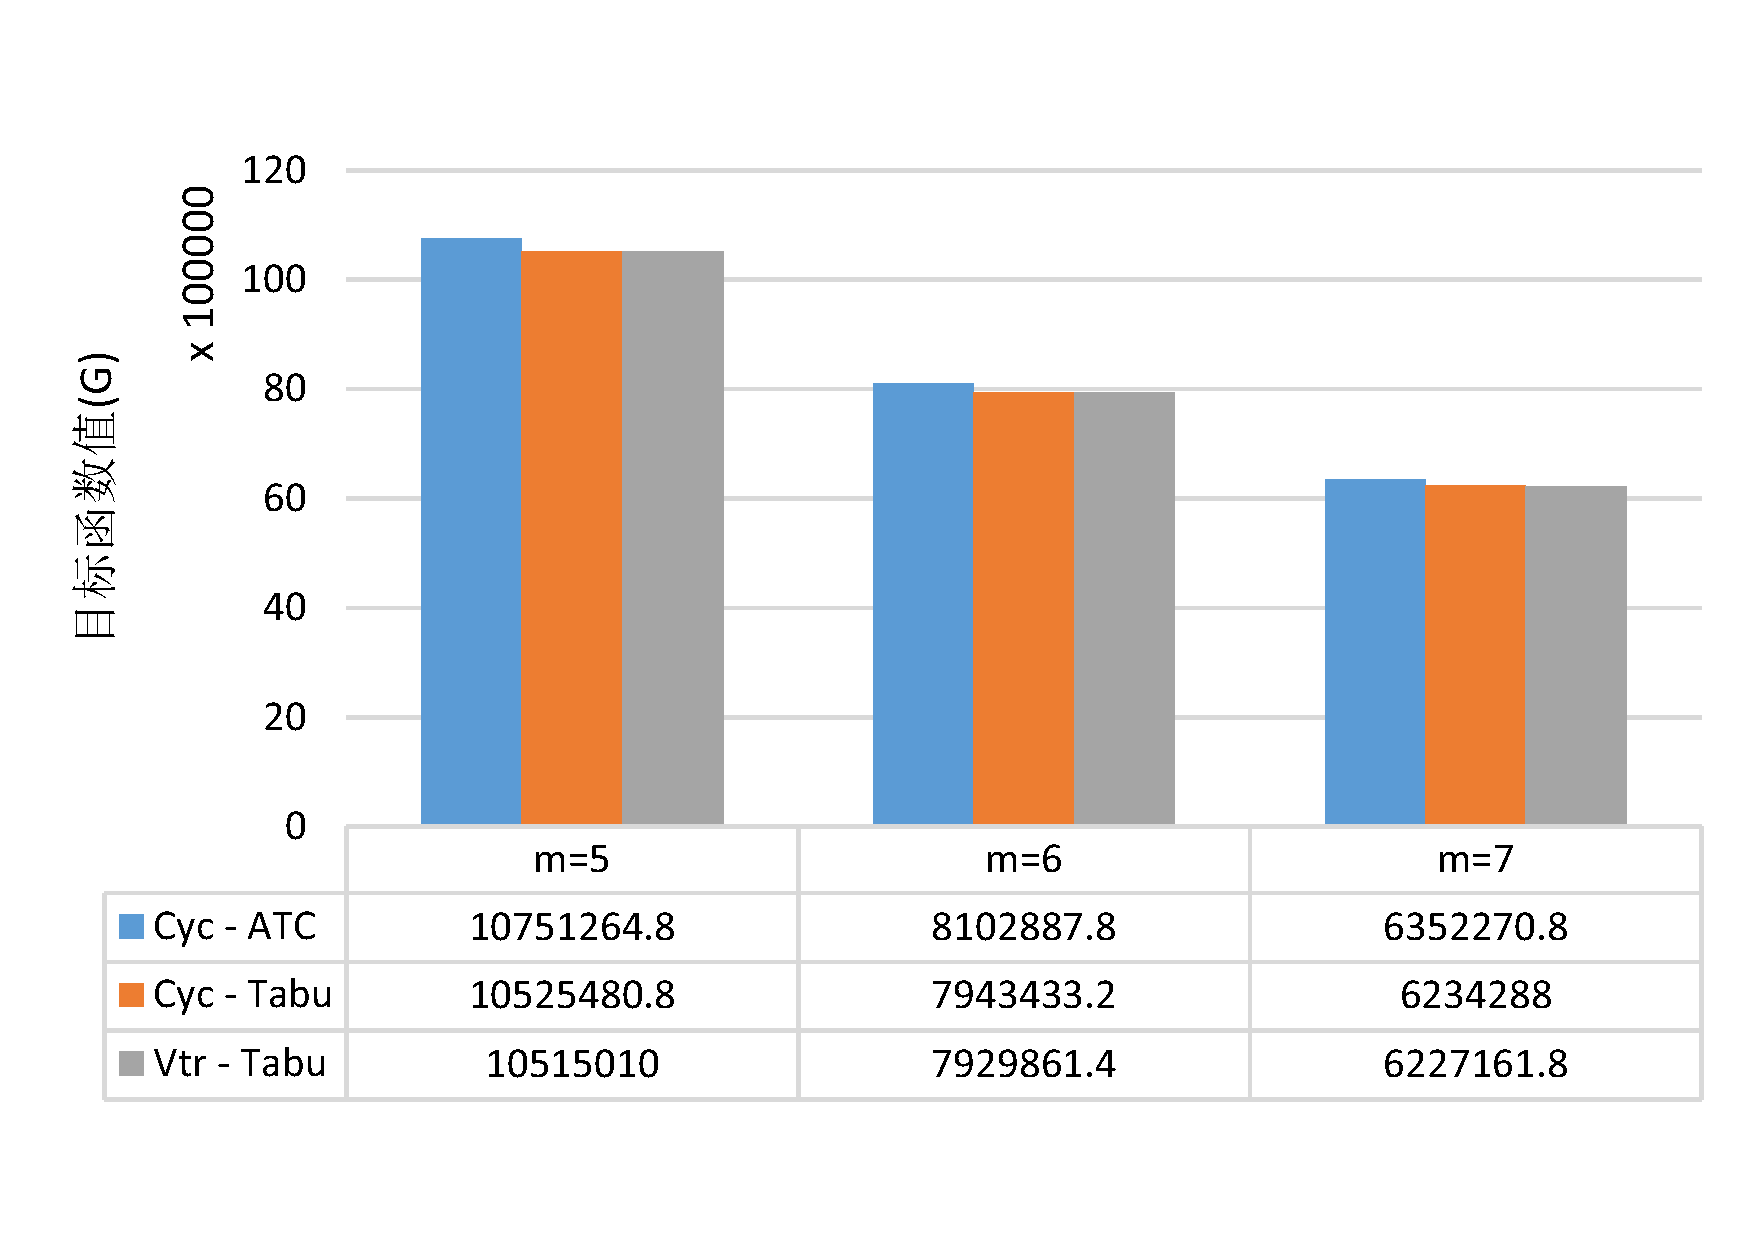
\includegraphics[height = 6cm, angle = -90]{basic_06_1000}}
\caption{\label{fig:result3}模型$1$的Cyc -- ATC、Cyc -- Tabu、Vtr -- Tabu 算法求解目标函数值比较$(\lambda_1 = 0.6)$}
\end{sidewaysfigure}

% !Mode:: "TeX:UTF-8"
% !TEX root = ..\thesis.tex
\begin{table}
\centering
\caption{Cyc -- ATC、Cyc -- Tabu、Vtr -- Tabu 算法求解模型1 目标函数值($\lambda_1 = 0.6$)}
\subfloat{
\begin{tabular}{cccccccc}
\toprule
流水线数量($m$) & 订单数量($n$) &$ 20    $&$ 30    $&$ 50    $&$ 70    $&$ 100   $&$ 150$ \\
\midrule
\multirow{3}[0]{*}{$5$} & Cyc - ATC &$ 3979  $&$ 8370  $&$ 26774 $&$ 45346 $&$ 90093 $&$ 239988$ \\
      & Cyc - Tabu &$ 3398  $&$ 6748.4 $&$ 21232.8 $&$ 34101.6 $&$ 69637.2 $&$ 181149.8$ \\
      & Vtr - Tabu&$ 2879  $&$ 5513.6 $&$ 17838.6 $&$ 27880.8 $&$ 56550.8 $&$ 140845$ \\
\multirow{3}[0]{*}{$6$} & Cyc - ATC &$ 3479  $&$ 7559.6 $&$ 24788.4 $&$ 42638.4 $&$ 85900.6 $&$ 230249.8$ \\
      & Cyc - Tabu &$ 2892  $&$ 5989.4 $&$ 18942.6 $&$ 31583.8 $&$ 64054.4 $&$ 173082.8$ \\
      & Vtr - Tabu &$ 2476  $&$ 4950.8 $&$ 15016.2 $&$ 24862 $&$ 50237.6 $&$ 133010.8$ \\
\multirow{3}[0]{*}{$7$} & Cyc - ATC &$ 3329  $&$ 7344.2 $&$ 24226.8 $&$ 42111.8 $&$ 85206 $&$ 229791.6$ \\
      & Cyc - Tabu &$ 2713  $&$ 5734.2 $&$ 18603.4 $&$ 31159.2 $&$ 63463.2 $&$ 172252.6$ \\
      & Vtr - Tabu &$ 2393  $&$ 4828.8 $&$ 14815.8 $&$ 24576.8 $&$ 49883.2 $&$ 132305.6$ \\
\bottomrule
\end{tabular}
}\\
\subfloat{
\begin{tabular}{ccccccc}
\toprule
流水线数量($m$) & 订单数量($n$) &$ 200   $&$ 300   $&$ 500   $&$ 750   $&$ 1000$ \\
\midrule
\multirow{3}[0]{*}{$5$} & Cyc - ATC &$ 440392 $&$ 971742 $&$ 2695817 $&$ 5999707 $&$ 10751265$ \\
      & Cyc - Taub&$ 336759 $&$ 742976.2 $&$ 2061723.8 $&$ 4539470.4 $&$ 8102887.8$ \\
      & Vtr - Tabu&$ 269899.6 $&$ 588606.2 $&$ 1626127.4 $&$ 3549589.2 $&$ 6352270.8$ \\
\multirow{3}[0]{*}{$6$} & Cyc - ATC &$ 423184.6 $&$ 936107.4 $&$ 2621922.8 $&$ 5841186.6 $&$ 10525481$ \\
      & Cyc - Tabu &$ 336759 $&$ 709764 $&$ 2002036.6 $&$ 4426885.4 $&$ 7943433.2$ \\
      & Vtr - Tabu &$ 269899.6 $&$ 561223 $&$ 1557005.6 $&$ 3447986.4 $&$ 6234288$ \\
\multirow{3}[0]{*}{$7$} & Cyc - ATC &$ 420668 $&$ 934482.8 $&$ 2616267 $&$ 5833132.2 $&$ 10515010$ \\
      & Cyc - Tabu &$ 318062.8 $&$ 706813 $&$ 1994074.6 $&$ 4420373.2 $&$ 7929861.4$ \\
      & Vtr - Tabu &$ 250808.8 $&$ 557683.6 $&$ 1553872.6 $&$ 3435631.6 $&$ 6227161.8$ \\
\bottomrule
\end{tabular}
}
\label{tab:resultmodel106}
\end{table}
% !Mode:: "TeX:UTF-8"
% !TEX root = ..\thesis.tex
\begin{table}
\centering
\caption{Cyc -- ATCS、Cyc -- Tabu、VVT 算法求解模型2 目标函数值($\lambda_1 = 0.4$)}
\subfloat{
\begin{tabular}{ccccrccc}
\toprule
流水线数量($m$) & 订单数量($n$) &$ 20    $&$ 30    $& $
50 $&$ 70    $&$ 100   $&$ 150$ \\
\midrule
\multirow{3}[0]{*}{$5$} & Cyc - ATCS &$ 6487  $&$ 14639 $&$ 36555.939 $&$ 58341 $&$ 123121 $&$ 293258$ \\
      & Cyc - Tabu &$ 3850  $&$ 7851.1783 $&$ 26889.191 $&$ 49564.683 $&$ 87671.223 $&$ 219358.13$ \\
      & VVT   &$ 3913  $&$ 8657.367 $&$ 28276.459 $&$ 42605.208 $&$ 93005.172 $&$ 210875.07$ \\
\multirow{3}[0]{*}{$6$} & Cyc - ATCS &$ 5855  $&$ 13784.833 $&$ 33917.555 $&$ 49510.443 $&$ 114232.19 $&$ 253435.71$ \\
      & Cyc - Tabu &$ 3510  $&$ 8203.5114 $&$ 25805.795 $&$ 52971.678 $&$ 85476.17 $&$ 202066.4$ \\
      & VVT   &$ 3588  $&$ 6477.6687 $&$ 21340.601 $&$ 42056.736 $&$ 82513.202 $&$ 159408.82$ \\
\multirow{3}[0]{*}{$7$} & Cyc - ATCS &$ 5788  $&$ 12887.76 $&$ 32360.801 $&$ 46228.992 $&$ 106777.75 $&$ 223006.92$ \\
      & Cyc - Tabu &$ 4291  $&$ 11239.113 $&$ 26888.348 $&$ 50925.934 $&$ 77160.63 $&$ 203876.09$ \\
      & VVT   &$ 3833  $&$ 7233.7701 $&$ 17850.436 $&$ 35495.155 $&$ 56956.974 $&$ 136442.08$ \\
\bottomrule
\end{tabular}
}\\
\subfloat{
\begin{tabular}{ccccccc}
\toprule
流水线数量($m$) & 订单数量($n$) &$ 200   $&$ 300   $&$ 500 $&$ 750   $&$ 1000$ \\
\midrule
\multirow{3}[0]{*}{$5$} & Cyc - ATCS &$ 485767 $&$ 1253111 $&$ 3374782 $&$ 6813918 $&$ 13032226$ \\
      & Cyc - Tabu &$ 428398.75 $&$ 1008863.9 $&$ 3285292 $&$ 6429213.5 $&$ 12999611$ \\
      & VVT   &$ 425257.79 $&$ 1117715 $&$ 3247024.2 $&$ 6571784.7 $&$ 12775684$ \\
\multirow{3}[0]{*}{$6$} & Cyc - ATCS &$ 450278.41 $&$ 1158313.9 $&$ 2947068.7 $&$ 6029824.6 $&$ 13032226$ \\
      & Cyc - Tabu &$ 425128.66 $&$ 1010966.5 $&$ 3156466.8 $&$ 6548880.6 $&$ 13017346$ \\
      & VVT   &$ 366877.04 $&$ 899843.51 $&$ 2810177.5 $&$ 5811671.2 $&$ 11730364$ \\
\multirow{3}[0]{*}{$7$} & Cyc - ATCS &$ 418525.84 $&$ 1041394.1 $&$ 2719254.5 $&$ 5478189.9 $&$ 13032226$ \\
      & Cyc - Tabu &$ 427484.09 $&$ 1135275.1 $&$ 3239972.4 $&$ 6682657.6 $&$ 12939689$ \\
      & VVT   &$ 311193.2 $&$ 943551.23 $&$ 2583663.4 $&$ 5297965.8 $&$ 10564891$ \\
\bottomrule
\end{tabular}
}
\label{tab:resultmodel204}
\end{table}
\begin{sidewaysfigure}
\centering
\subfloat[$n = 20$]{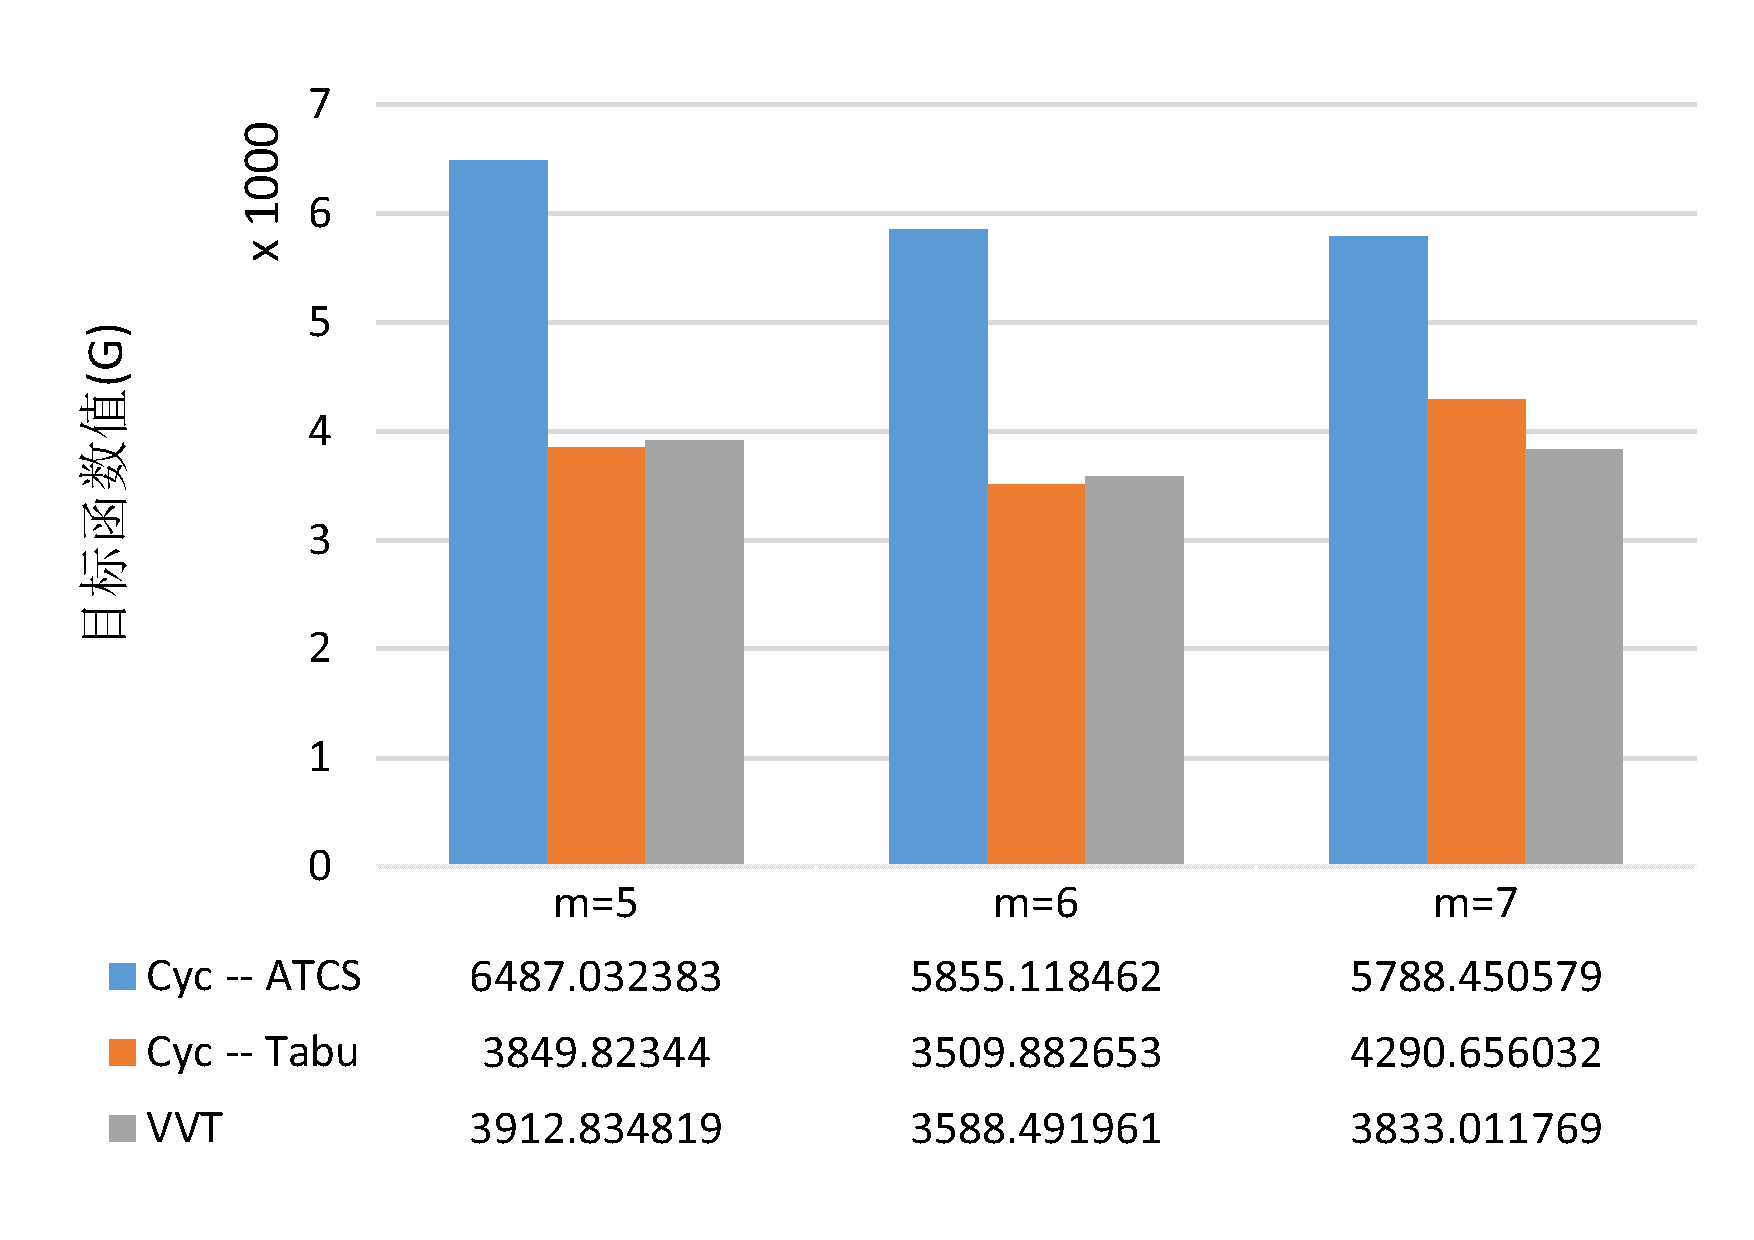
\includegraphics[height = 6cm, angle = -90]{continue_04_20}}
\subfloat[$n = 30$]{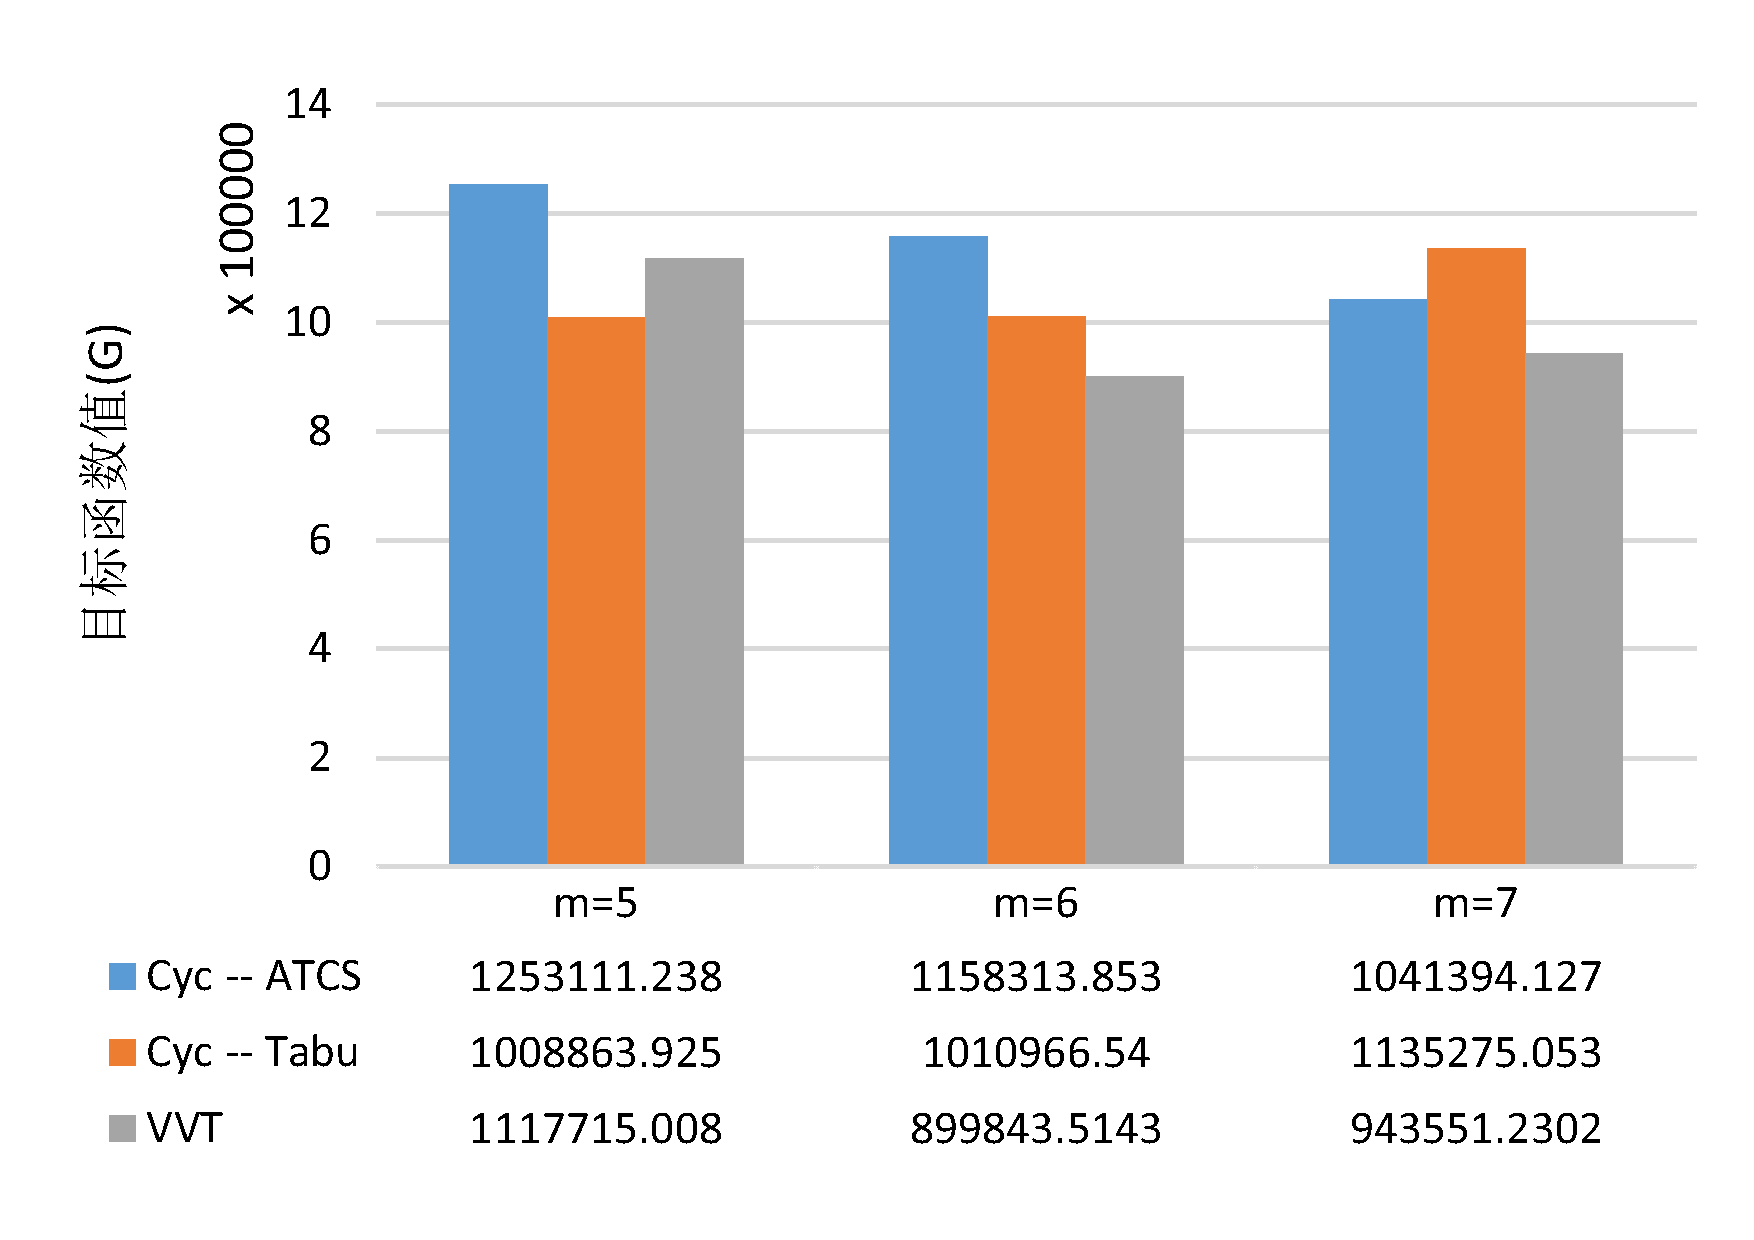
\includegraphics[height = 6cm, angle = -90]{continue_04_300}}
\subfloat[$n = 50$]{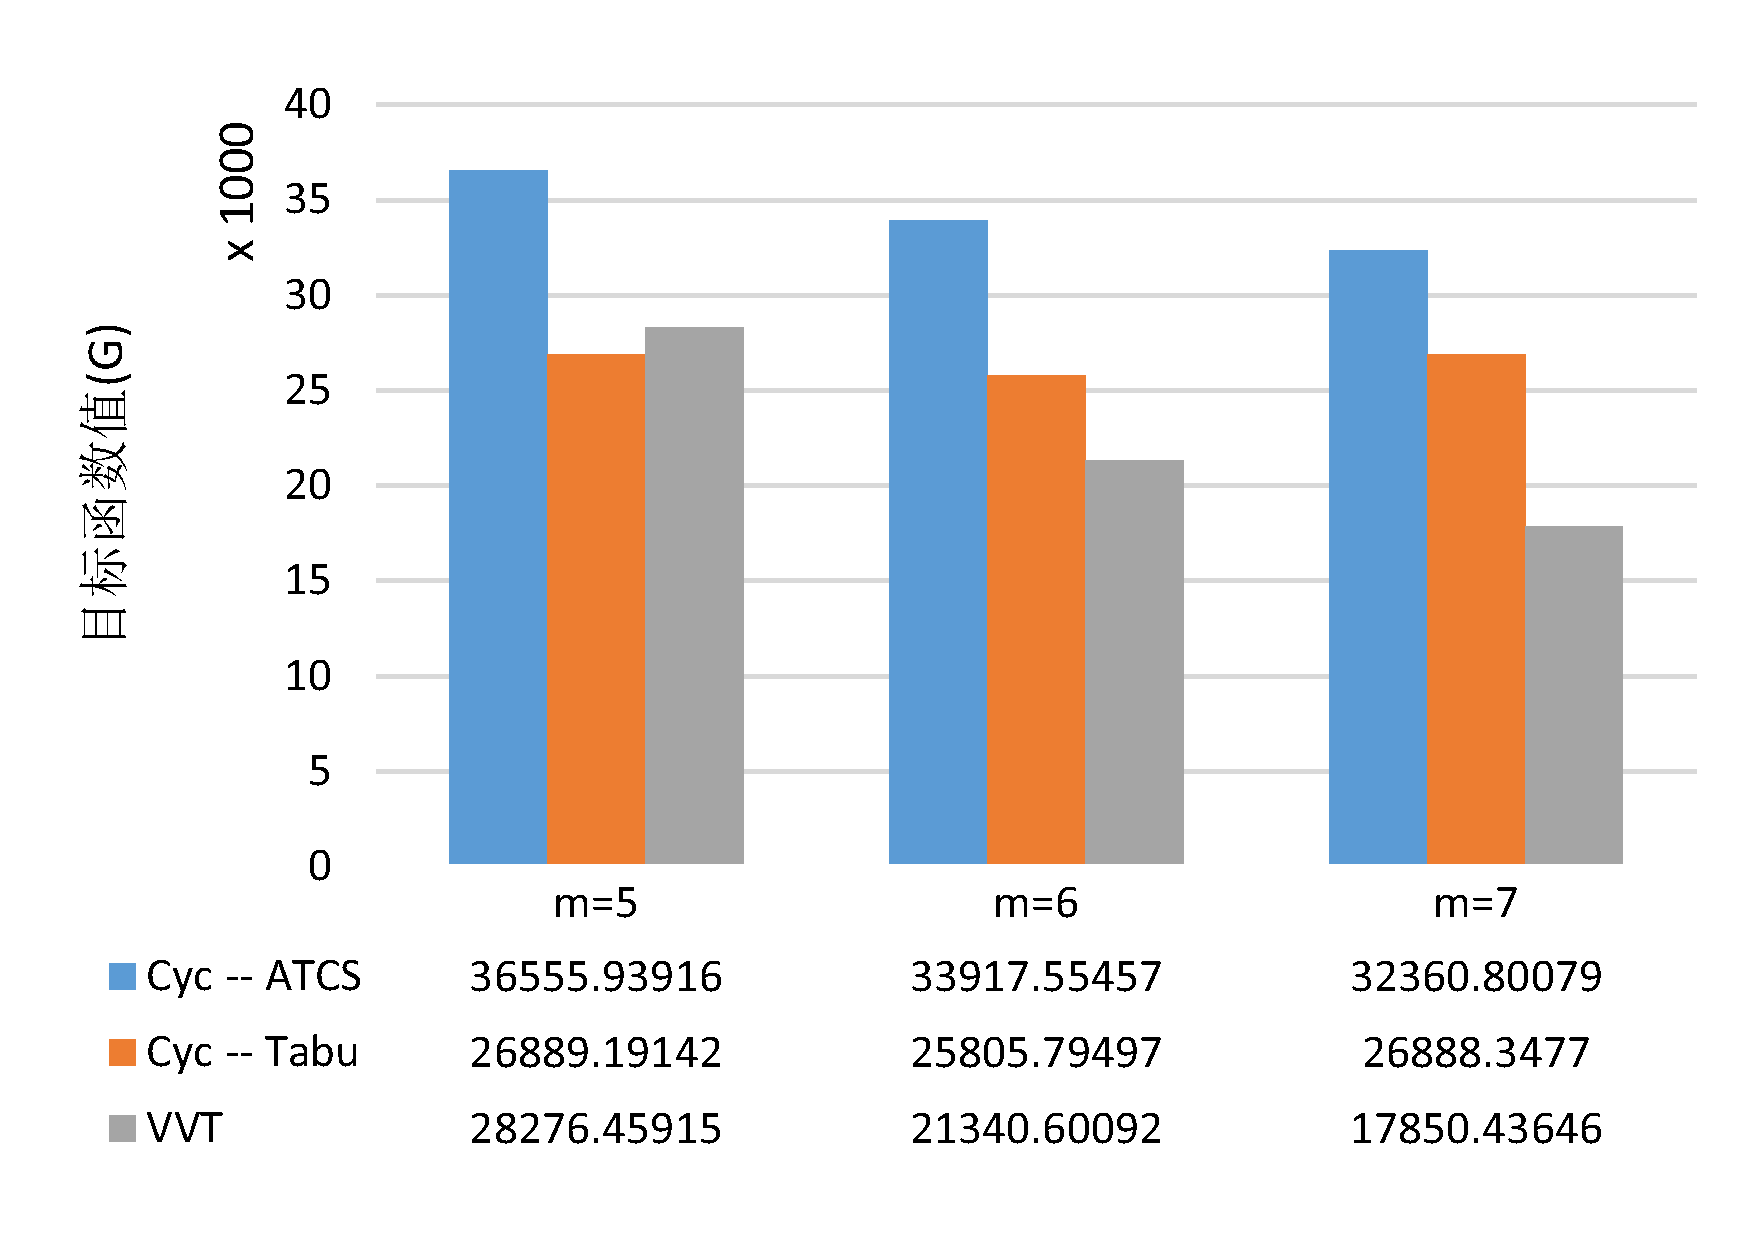
\includegraphics[height = 6cm, angle = -90]{continue_04_50}}
\subfloat[$n = 70$]{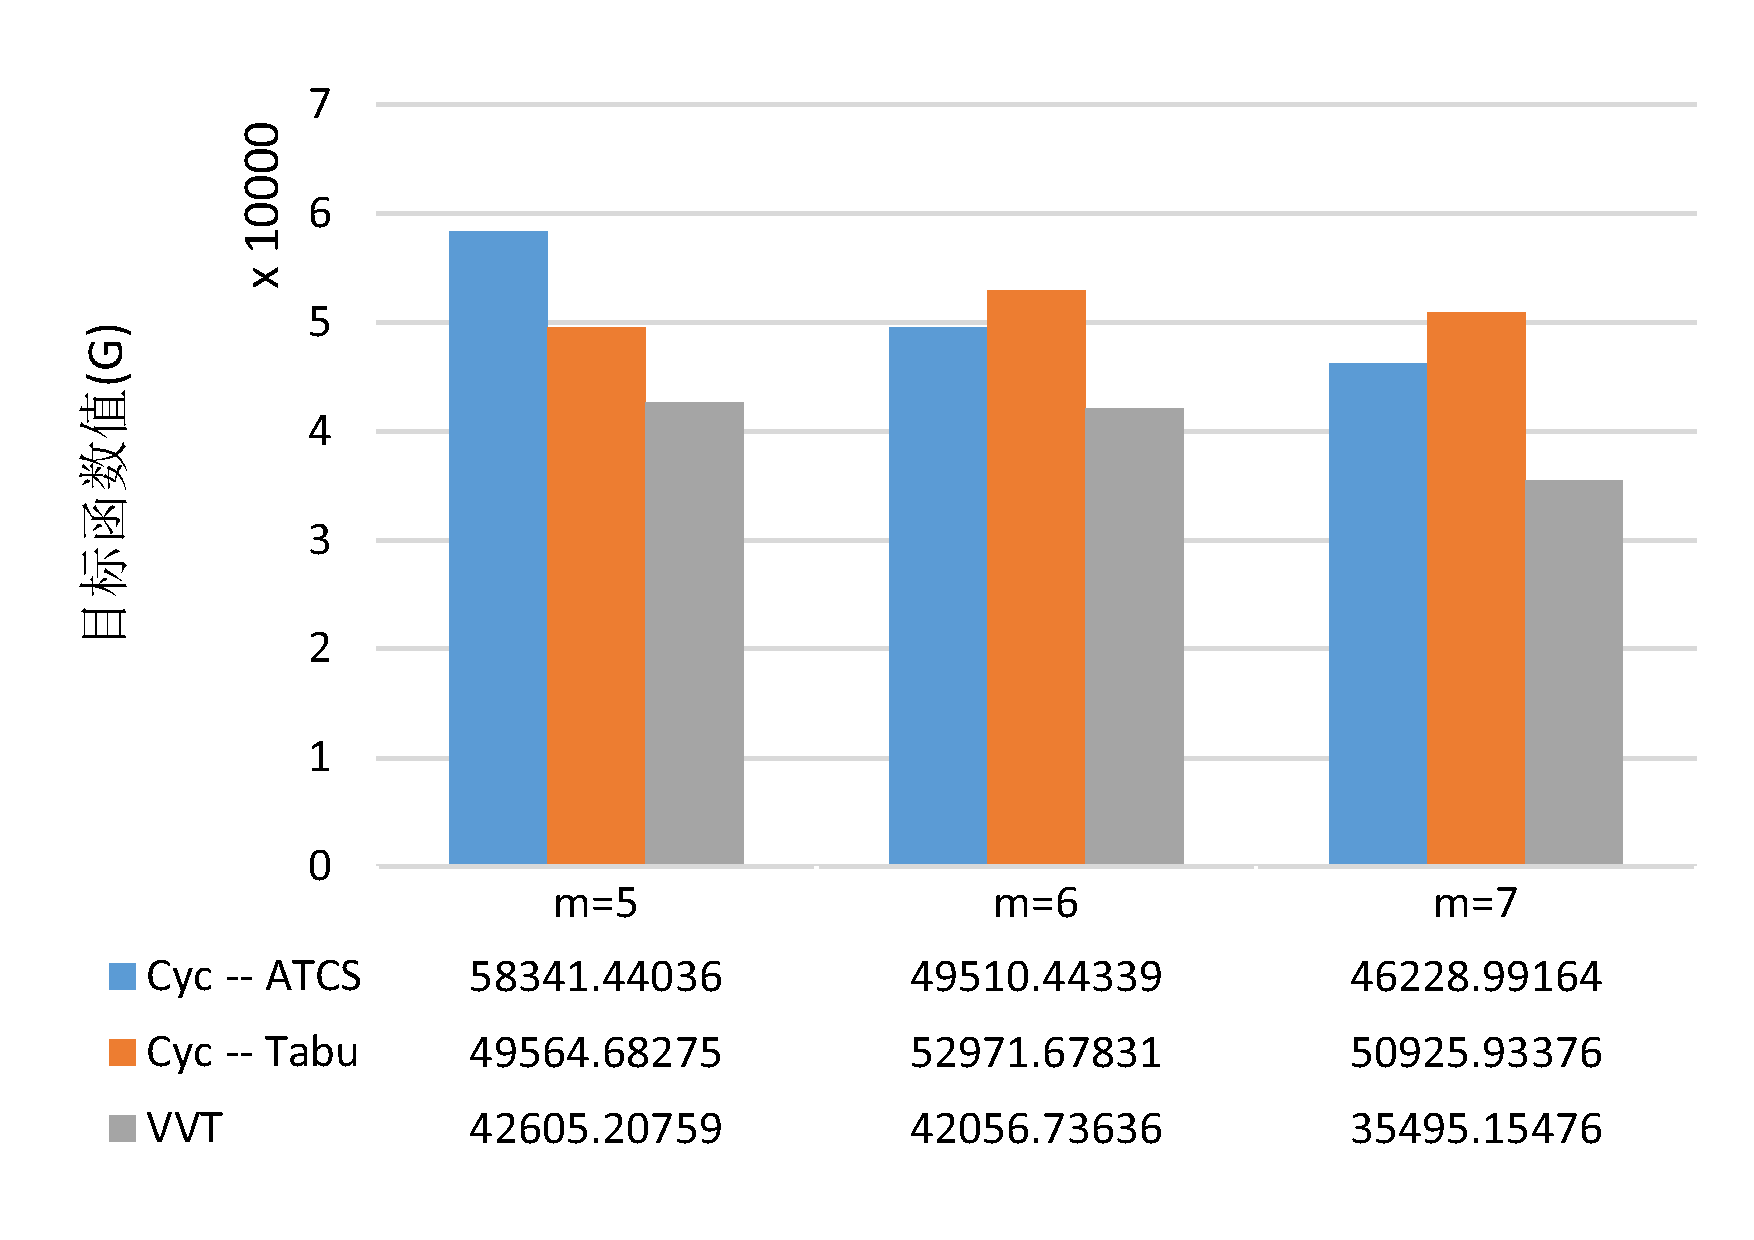
\includegraphics[height = 6cm, angle = -90]{continue_04_70}}\\
\subfloat[$n = 100$]{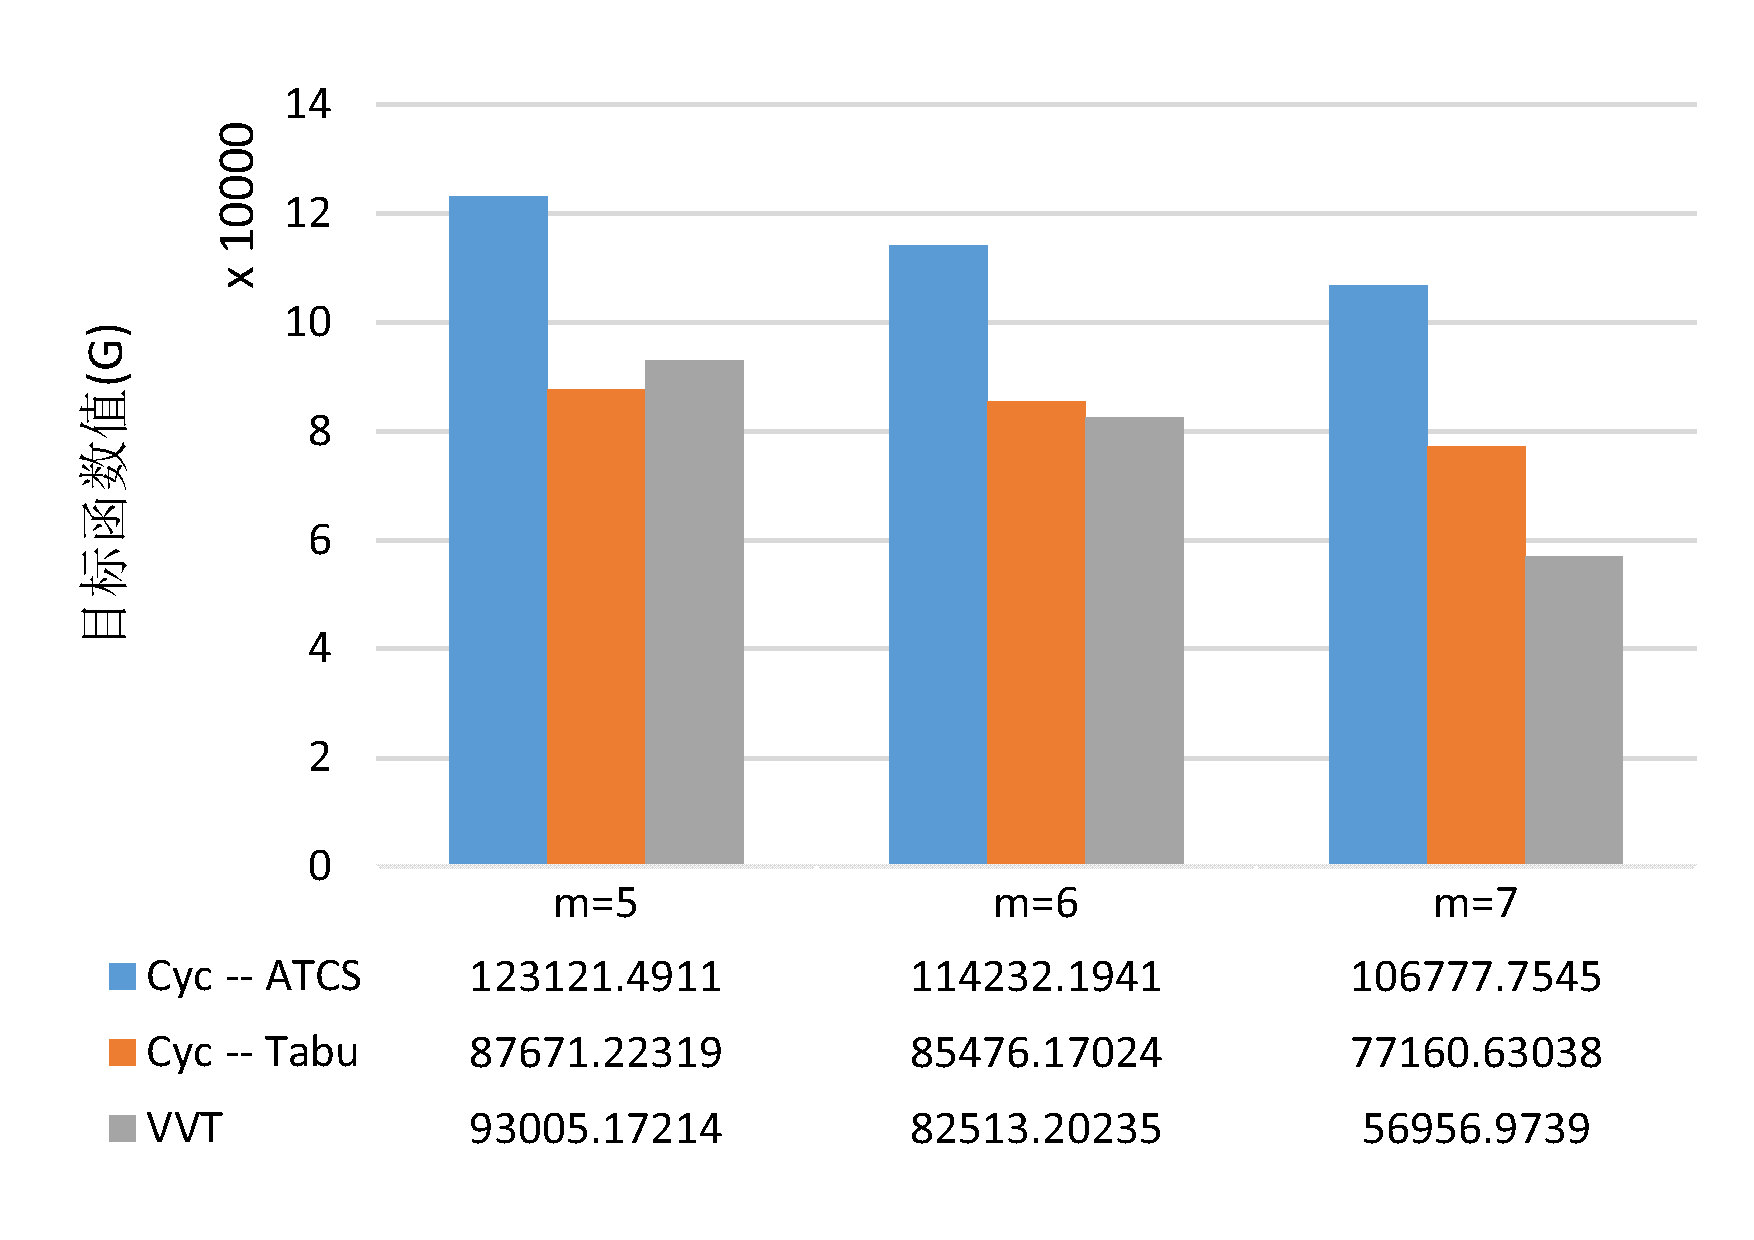
\includegraphics[height = 6cm, angle = -90]{continue_04_100}}
\subfloat[$n = 150$]{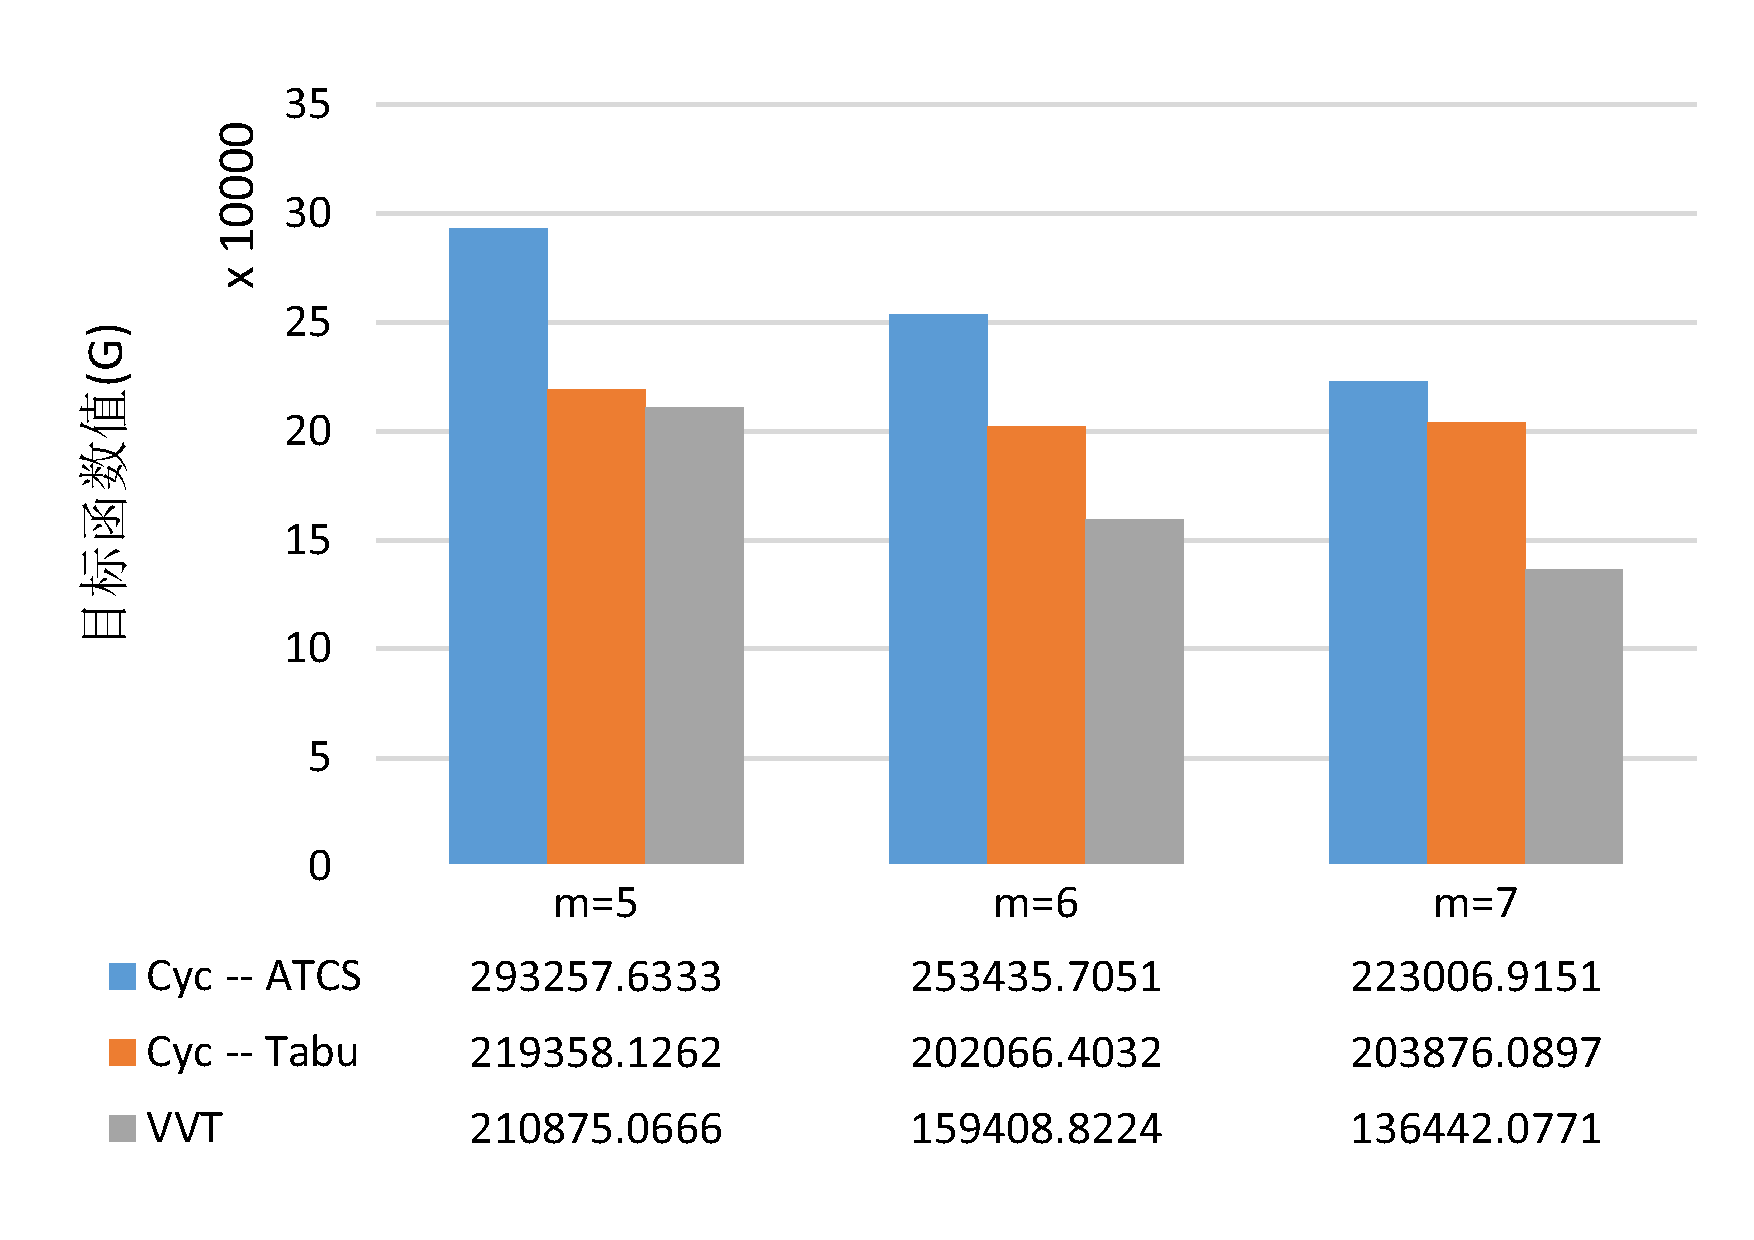
\includegraphics[height = 6cm, angle = -90]{continue_04_150}}
\subfloat[$n = 200$]{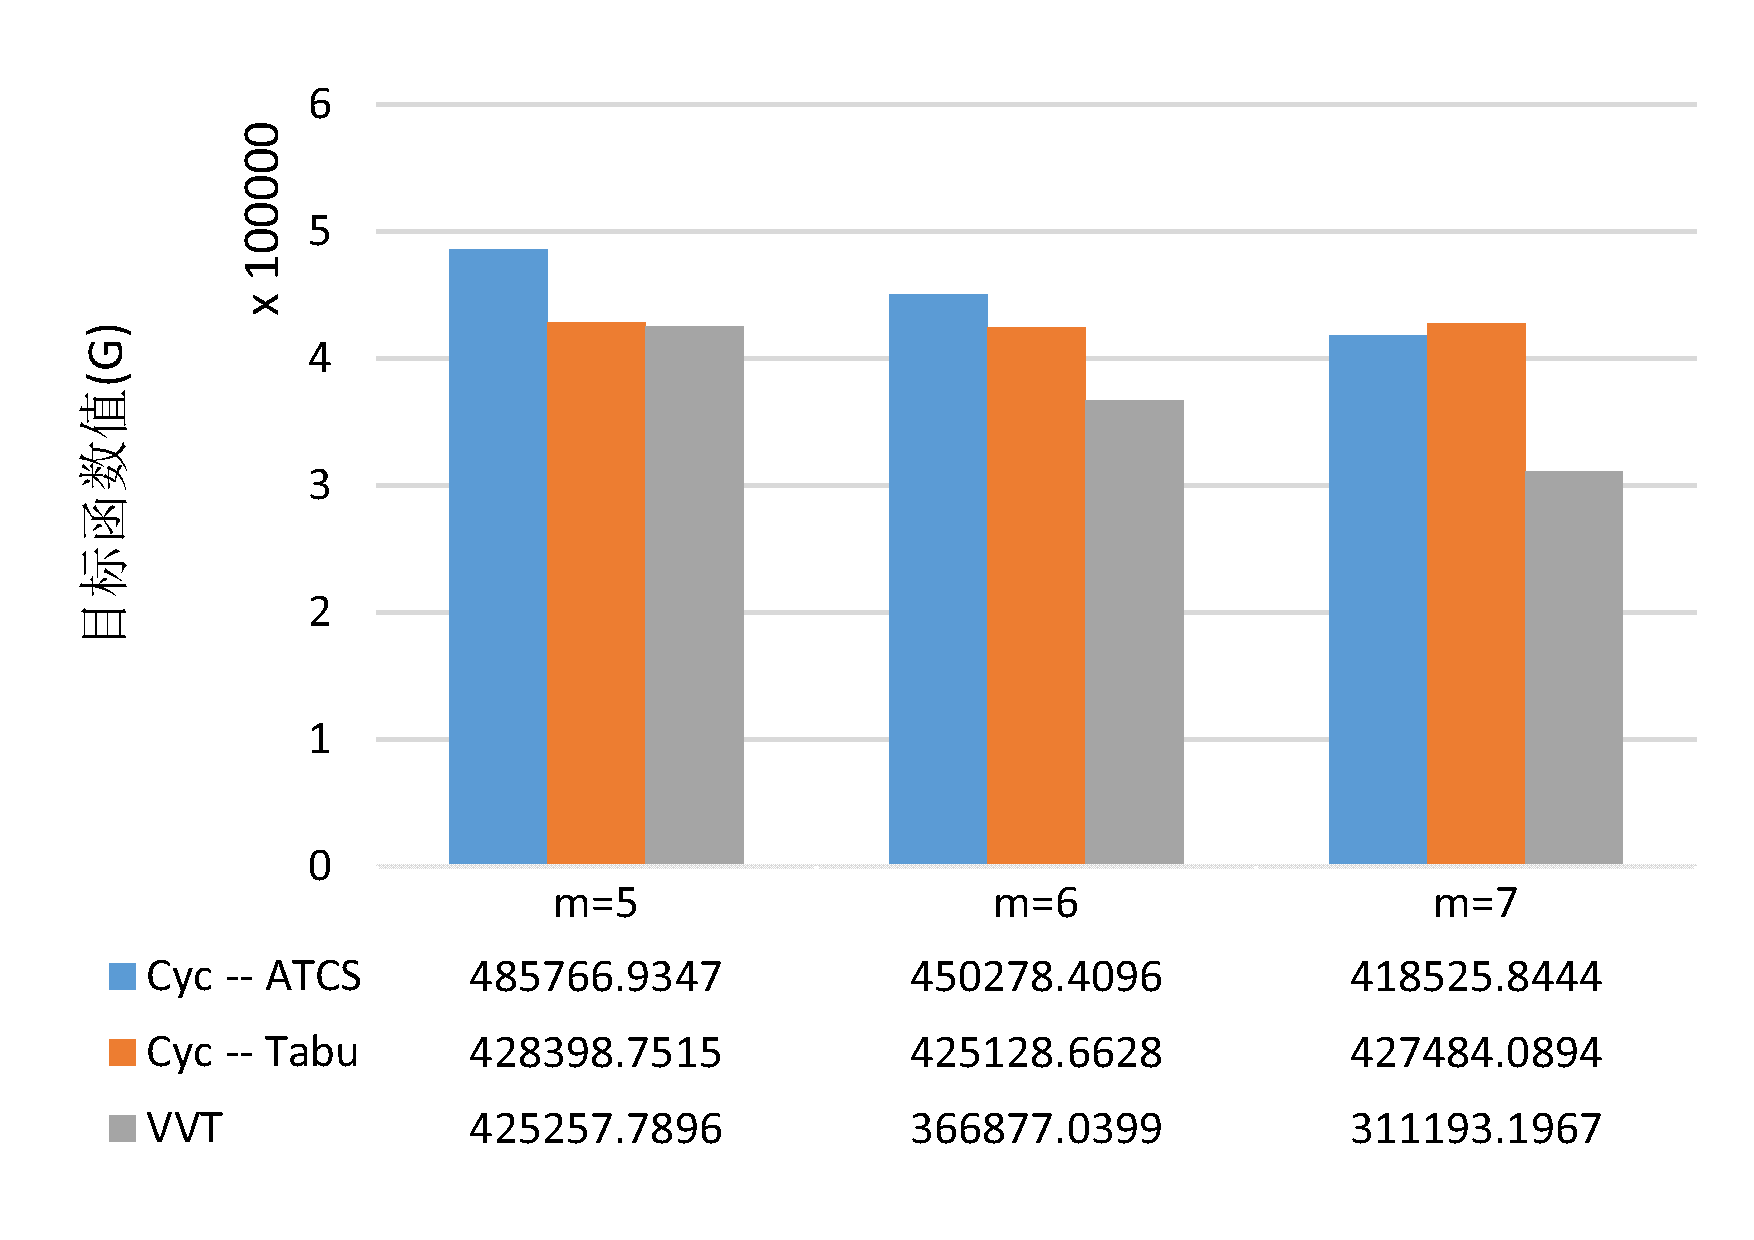
\includegraphics[height = 6cm, angle = -90]{continue_04_200}}
\subfloat[$n = 300$]{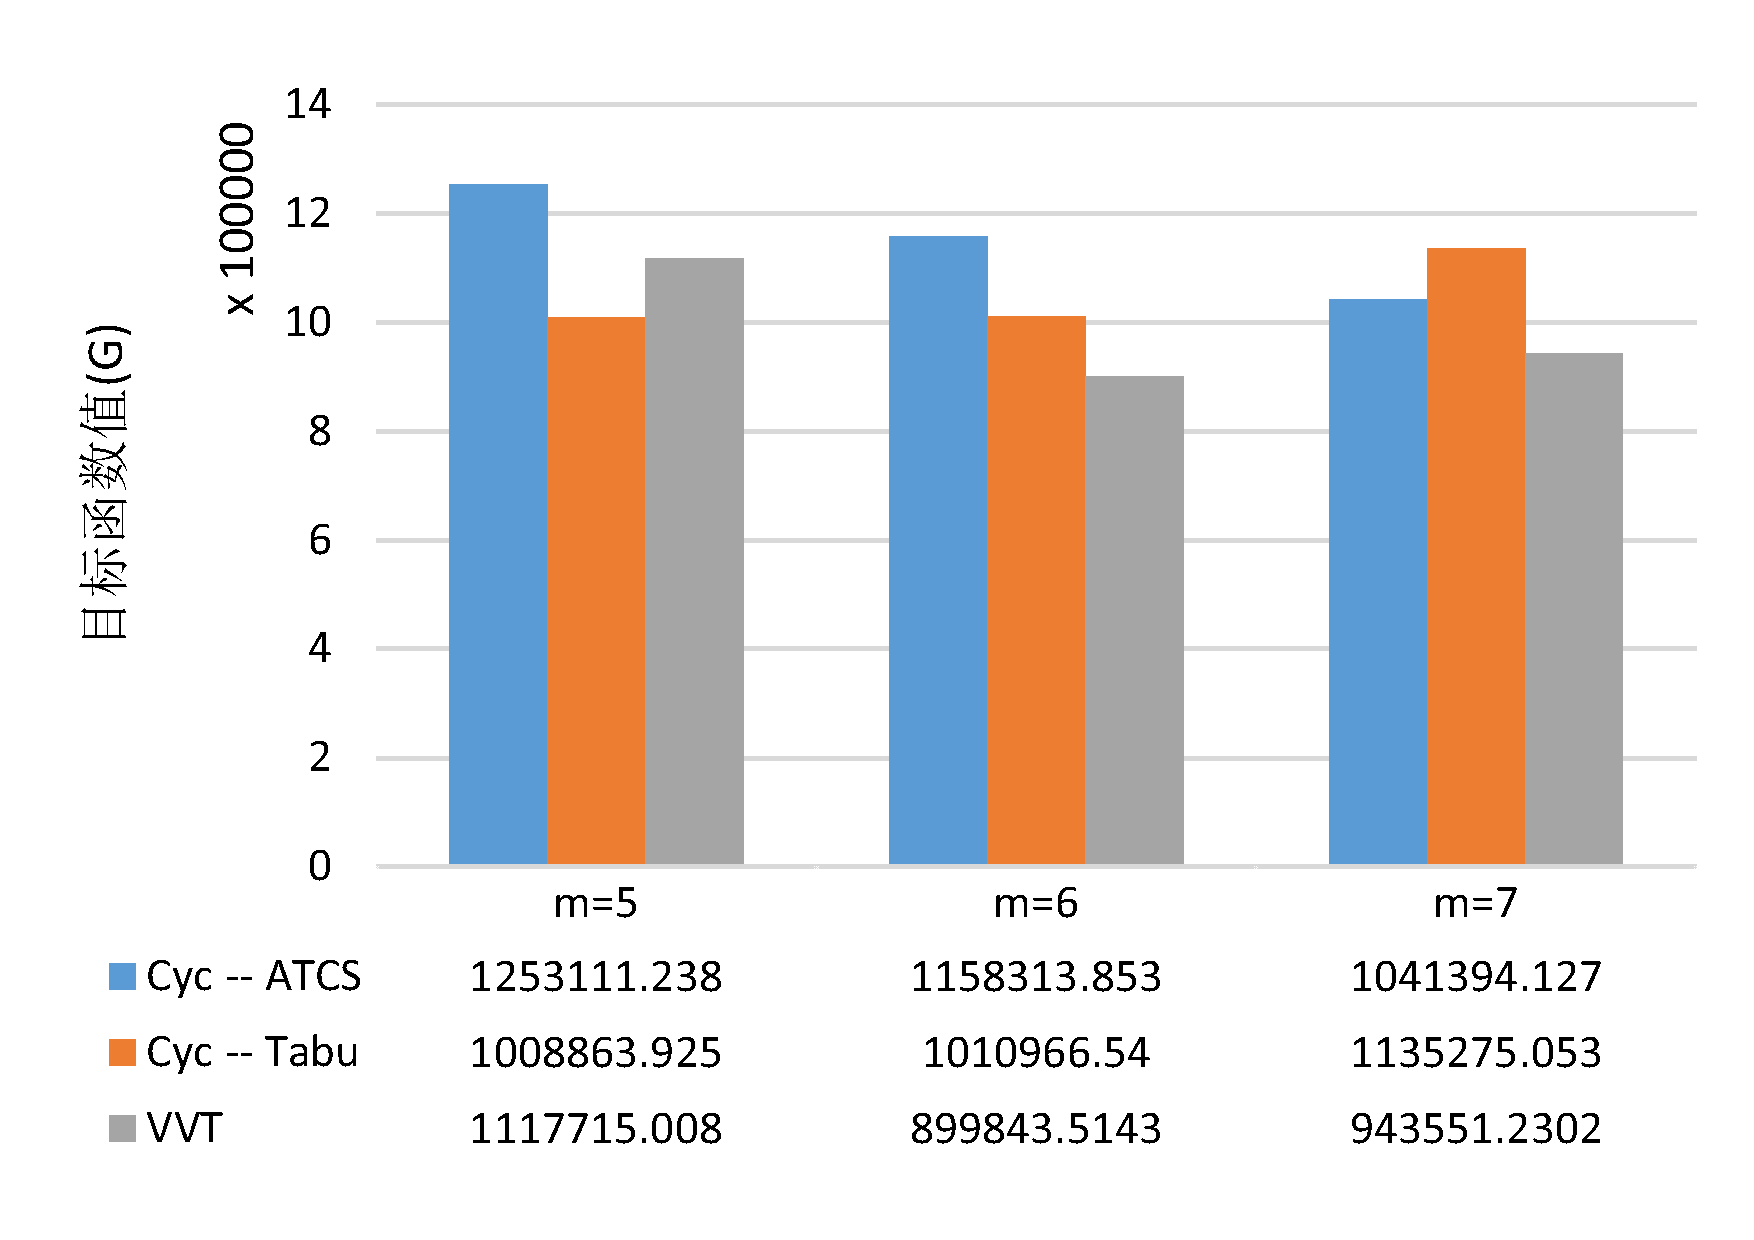
\includegraphics[height = 6cm, angle = -90]{continue_04_300}}\\
\subfloat[$n = 500$]{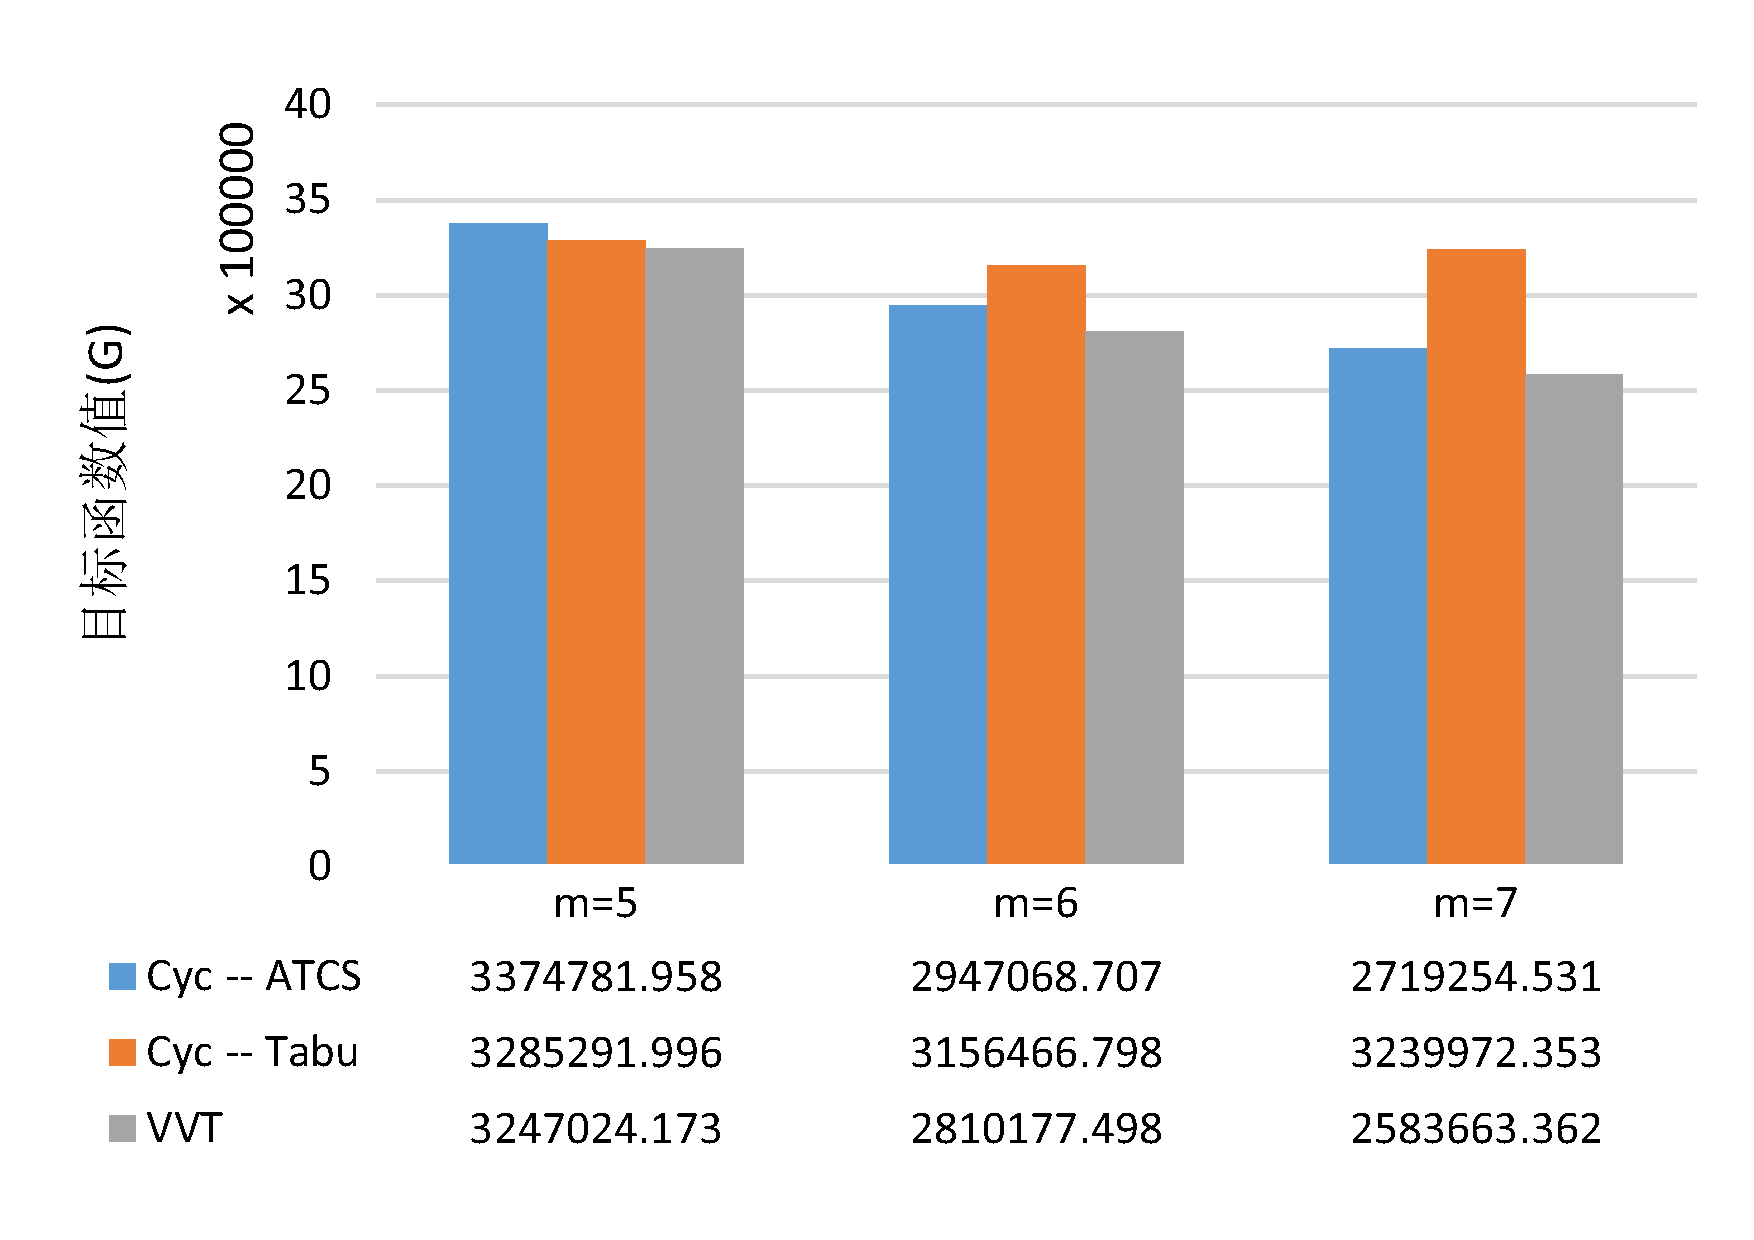
\includegraphics[height = 6cm, angle = -90]{continue_04_500}}
\subfloat[$n = 750$]{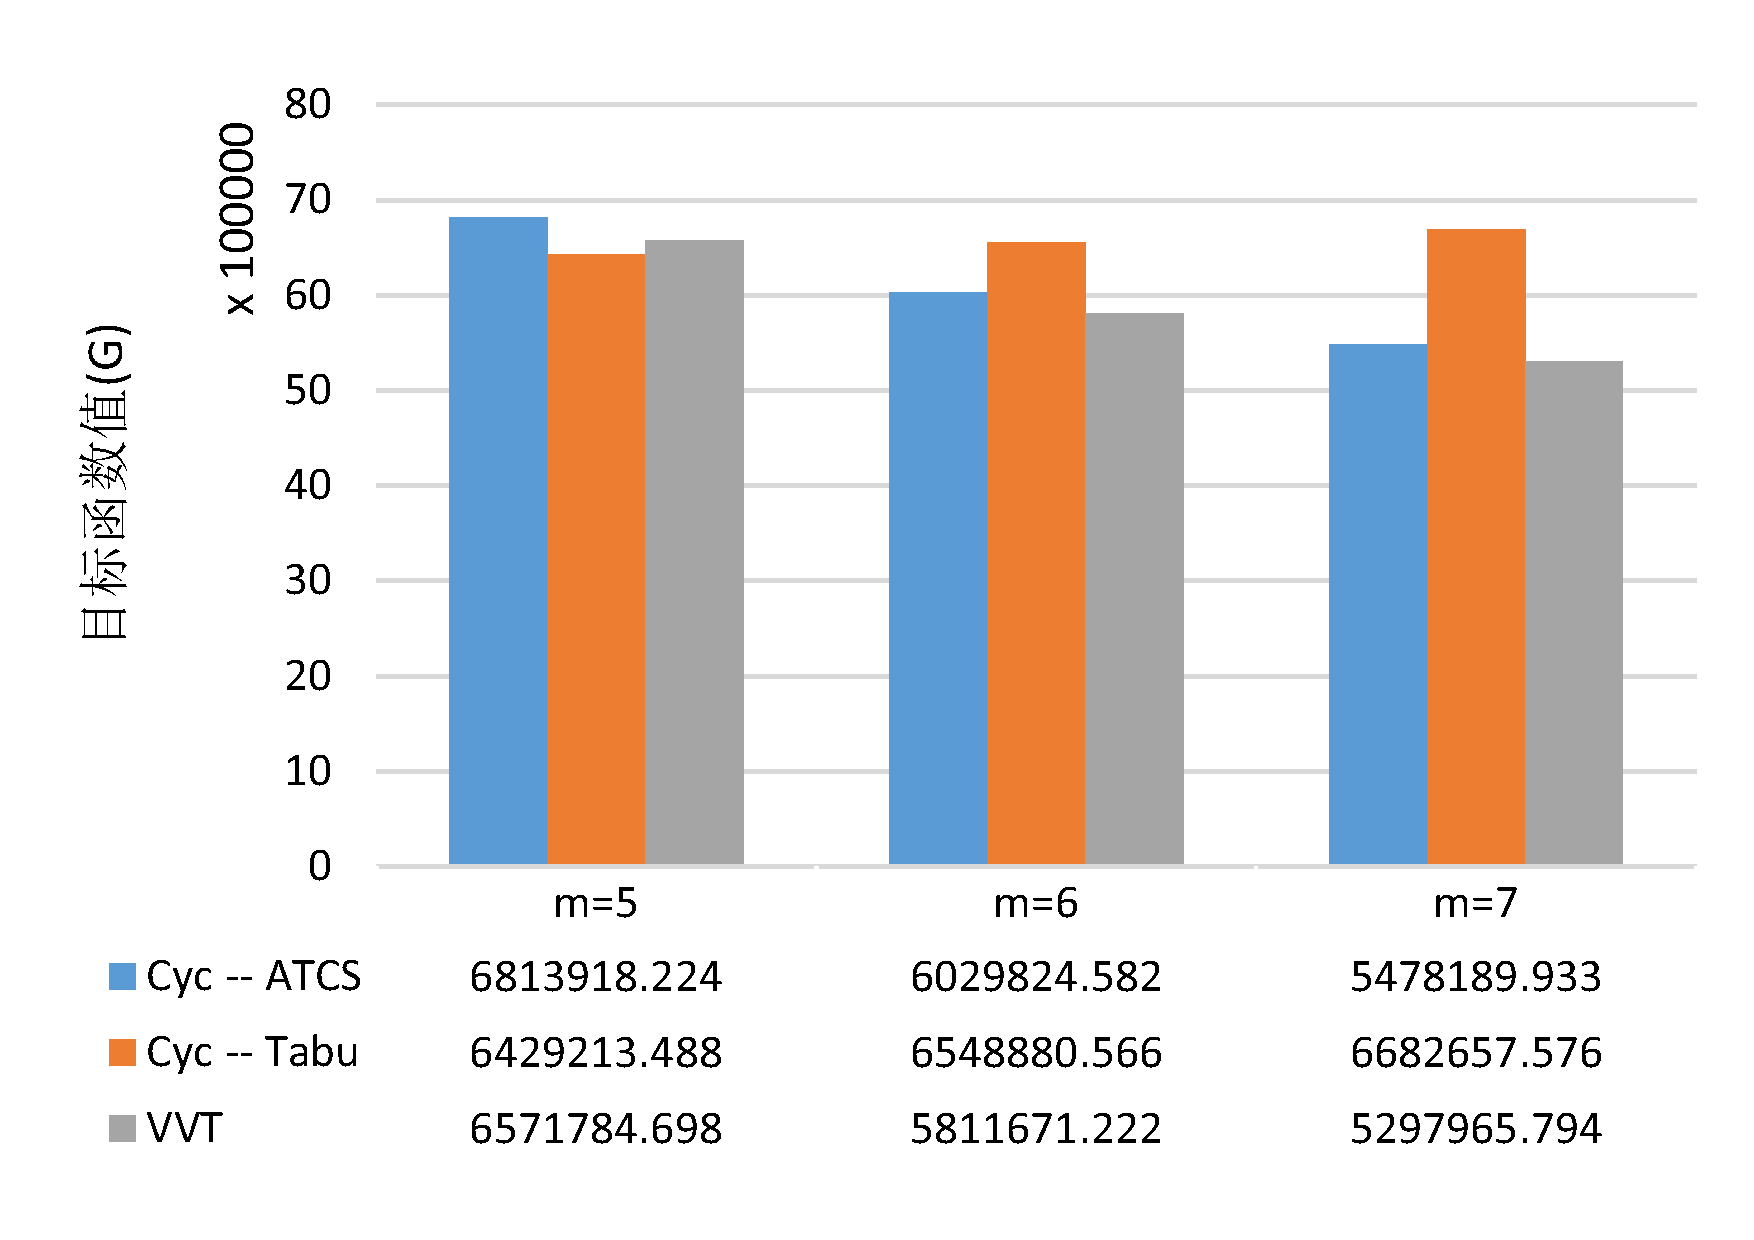
\includegraphics[height = 6cm, angle = -90]{continue_04_750}}
\subfloat[$n = 1000$]{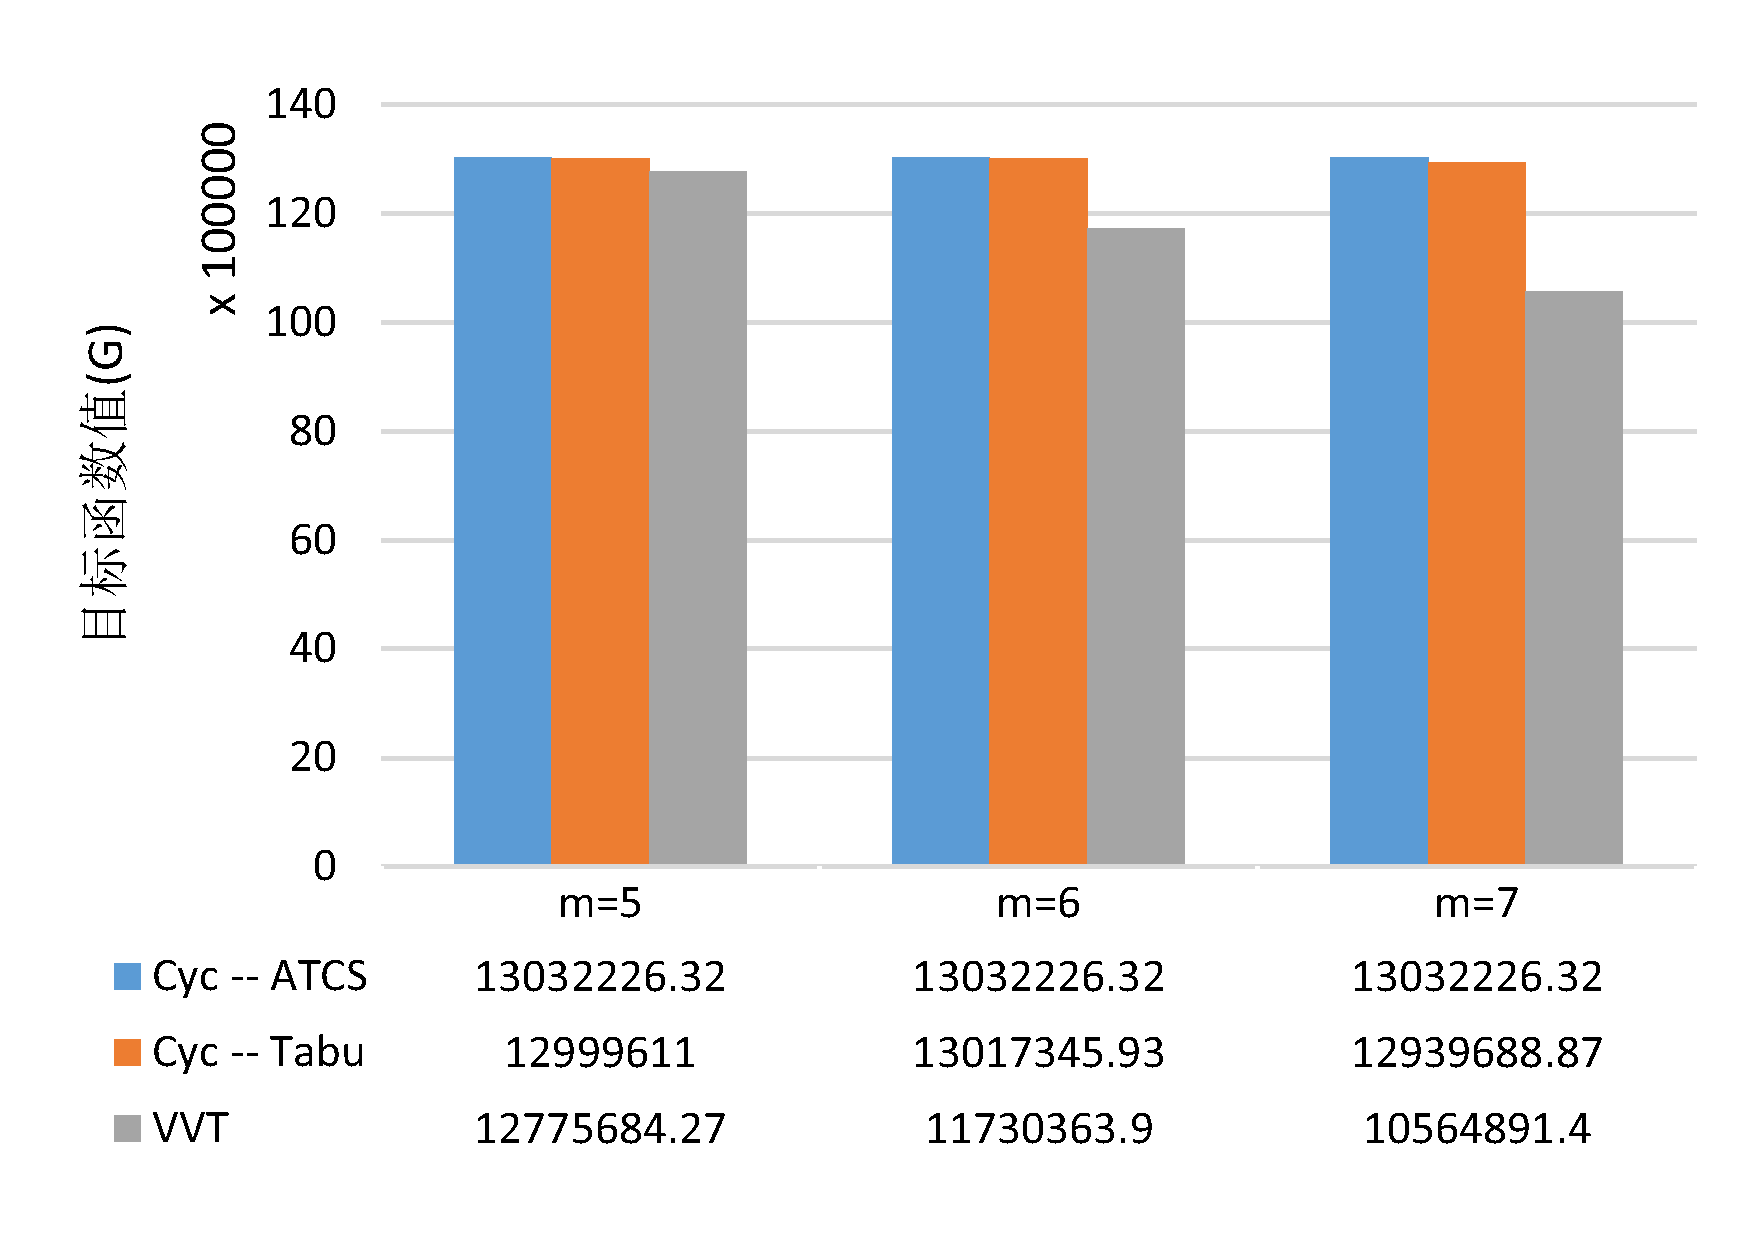
\includegraphics[height = 6cm, angle = -90]{continue_04_1000}}
\caption{\label{fig:result4}模型$2$的Cyc -- ATCS、Cyc -- Tabu、VVT 算法求解目标函数值比较$(\lambda_1 = 0.4)$}
\end{sidewaysfigure}

% !Mode:: "TeX:UTF-8"
% !TEX root = ..\thesis.tex
\begin{table}
\centering
\caption{Cyc -- ATCS、Cyc -- Tabu、VVT 算法求解模型2 目标函数值($\lambda_1 = 0.5$)}
\subfloat{
\begin{tabular}{cccccccc}
\toprule
流水线数量($m$) & 订单数量($n$) &$ 20    $&$ 30    $&$ 50    $&$ 70    $&$ 100   $&$ 150$ \\
\midrule
\multirow{3}[0]{*}{$5$} & Cyc - ATCS &$ 6740  $&$ 15186 $&$ 38060 $&$ 61202 $&$ 133384 $&$ 314488$ \\
      & Cyc - Tabu &$ 3957  $&$ 7475.494 $&$ 30024.952 $&$ 43281.954 $&$ 89535.599 $&$ 230244.43$ \\
      & VVT   &$ 4841  $&$ 10682.449 $&$ 30334.404 $&$ 45382.031 $&$ 91565.783 $&$ 233094.79 $\\
\multirow{3}[0]{*}{$6$} & Cyc - ATCS &$ 6056  $&$ 14293.191 $&$ 35423.612 $&$ 51775.478 $&$ 122588.7 $&$ 271166.69$ \\
      & Cyc - Tabu &$ 3560  $&$ 7173.9686 $&$ 24593.106 $&$ 46707.875 $&$ 85702.282 $&$ 203873.55$ \\
      & VVT   &$ 3185  $&$ 5580.5588 $&$ 22762.927 $&$ 42459.636 $&$ 90951.2 $&$ 161589.65$ \\
\multirow{3}[0]{*}{$7$} & Cyc - ATCS &$ 5720  $&$ 13337.446 $&$ 34178.32 $&$ 49005.801 $&$ 113118.15 $&$ 237750.37$ \\
      & Cyc - Tabu &$ 5033  $&$ 10620.604 $&$ 25618.636 $&$ 48125.465 $&$ 93584.444 $&$ 205749.06$ \\
      & VVT   &$ 3805  $&$ 5781.3025 $&$ 18140.016 $&$ 36682.585 $&$ 53703.663 $&$ 134552.74$ \\
\bottomrule
\end{tabular}
}\\
\subfloat{
\begin{tabular}{ccccccc}
\toprule
流水线数量($m$) & 订单数量($n$) &$ 200   $&$ 300   $&$ 500   $&$ 750   $&$ 1000$ \\
\midrule
\multirow{3}[0]{*}{$5$} & Cyc - ATCS &$ 512529 $&$ 1337254 $&$ 3600003 $&$ 7235024 $&$ 13904592$ \\
      & Cyc - Tabu &$ 439460.13 $&$ 1102003.4 $&$ 3450126.4 $&$ 6756132 $&$ 13867215$ \\
      & VVT   &$ 450672.22 $&$ 1207918 $&$ 3465804.3 $&$ 6990151.6 $&$ 13738407$ \\
\multirow{3}[0]{*}{$6$} & Cyc - ATCS &$ 476880.16 $&$ 1234507.1 $&$ 3140292 $&$ 6447693.7 $&$ 13904592$ \\
      & Cyc - Tabu &$ 441373.17 $&$ 1097814.1 $&$ 3369450.8 $&$ 6989977.2 $&$ 13902982$ \\
      & VVT   &$ 391727.05 $&$ 974797.64 $&$ 2979827.2 $&$ 6136982.2 $&$ 12446438$ \\
\multirow{3}[0]{*}{$7$} & Cyc - ATCS &$ 436937.69 $&$ 1110805 $&$ 2895860.9 $&$ 5795939.3 $&$ 13904592$ \\
      & Cyc - Tabu &$ 442388.89 $&$ 1234795.9 $&$ 3502010 $&$ 7115955.3 $&$ 13774464$ \\
      & VVT   &$ 304350.76 $&$ 967481.18 $&$ 2737065 $&$ 5545648.9 $&$ 11242550$ \\
\bottomrule
\end{tabular}
}
\label{tab:resultmodel205}
\end{table}
% !Mode:: "TeX:UTF-8"
% !TEX root = ..\thesis.tex
\begin{table}
\centering
\caption{Cyc -- ATCS、Cyc -- Tabu、VVT 算法求解模型2 目标函数值($\lambda_1 = 0.6$)}
\subfloat{
\begin{tabular}{cccccccc}
\toprule
流水线数量($m$) & 订单数量($n$) &$ 20    $&$ 30    $&$ 50    $&$ 70    $&$ 100   $&$ 150$ \\
\midrule
\multirow{3}[0]{*}{$5$} & Cyc - ATCS &$ 6536  $&$ 15460 $&$ 39821 $&$ 64062 $&$ 138328 $&$ 334844$ \\
      & Cyc - Tabu &$ 4006  $&$ 8412.1974 $&$ 28282.738 $&$ 47732.025 $&$ 94457.323 $&$ 226605.08$ \\
      & VVT   &$ 4323  $&$ 7979.0224 $&$ 28277.507 $&$ 46135.165 $&$ 94500.141 $&$ 241701.07 $\\
\multirow{3}[0]{*}{$6$} & Cyc - ATCS &$ 6276  $&$ 14801.549 $&$ 36929.67 $&$ 54043.214 $&$ 129235.53 $&$ 288897.68$ \\
      & Cyc - Tabu &$ 3424  $&$ 8248.3767 $&$ 27369.773 $&$ 47279.659 $&$ 86141.272 $&$ 213476.86$ \\
      & VVT   &$ 3604  $&$ 5725.7217 $&$ 21615.213 $&$ 40028.772 $&$ 93898.487 $&$ 164785.29 $\\
\multirow{3}[0]{*}{$7$} & Cyc - ATCS &$ 6002  $&$ 13890.81 $&$ 36826.504 $&$ 50582.146 $&$ 119156.7 $&$ 252460.32$ \\
      & Cyc - Tabu &$ 4236  $&$ 8735.0075 $&$ 25470.642 $&$ 48098.666 $&$ 84992.165 $&$ 210151.94$ \\
      & VVT   &$ 3730  $&$ 6336.405 $&$ 19830.276 $&$ 37488.671 $&$ 57210.411 $&$ 142846.99$ \\
\bottomrule
\end{tabular}
}\\
\subfloat{
\begin{tabular}{ccccccc}
\toprule
流水线数量($m$) & 订单数量($n$) &$ 200   $&$ 300   $&$ 500   $&$ 750   $&$ 1000$ \\
\midrule
\multirow{3}[0]{*}{$5$} & Cyc - ATCS &$ 539637 $&$ 1421502 $&$ 3842180 $&$ 7681112 $&$ 14821505$ \\
      & Cyc - Tabu &$ 461679.68 $&$ 1190764.1 $&$ 3657340.3 $&$ 7177373.7 $&$ 14853646$ \\
      & VVT   &$ 483441.39 $&$ 1240203.6 $&$ 3687990.8 $&$ 7344367.5 $&$ 14621840$ \\
\multirow{3}[0]{*}{$6$} & Cyc - ATCS &$ 503521.09 $&$ 1310700.4 $&$ 3361729.1 $&$ 6829840.8 $&$ 14821505$ \\
      & Cyc - Tabu &$ 453662.49 $&$ 1113032.7 $&$ 3573224.3 $&$ 7318057.6 $&$ 14863523$ \\
      & VVT   &$ 391036.57 $&$ 993546.02 $&$ 3169608.7 $&$ 6478538.2 $&$ 13241260$ \\
\multirow{3}[0]{*}{$7$} & Cyc - ATCS &$ 458750.04 $&$ 1181963.8 $&$ 3080549.8 $&$ 6122988.8 $&$ 14821505$ \\
      & Cyc - Tabu &$ 454908.33 $&$ 1252287.2 $&$ 3646277.8 $&$ 7506555.2 $&$ 14656063$ \\
      & VVT   &$ 322579.1 $&$ 1065107.2 $&$ 2882401.5 $&$ 5924617.8 $&$ 11897569$ \\
\bottomrule
\end{tabular}
}
\label{tab:resultmodel206}
\end{table}
\begin{sidewaysfigure}
\centering
\subfloat[$n = 20$]{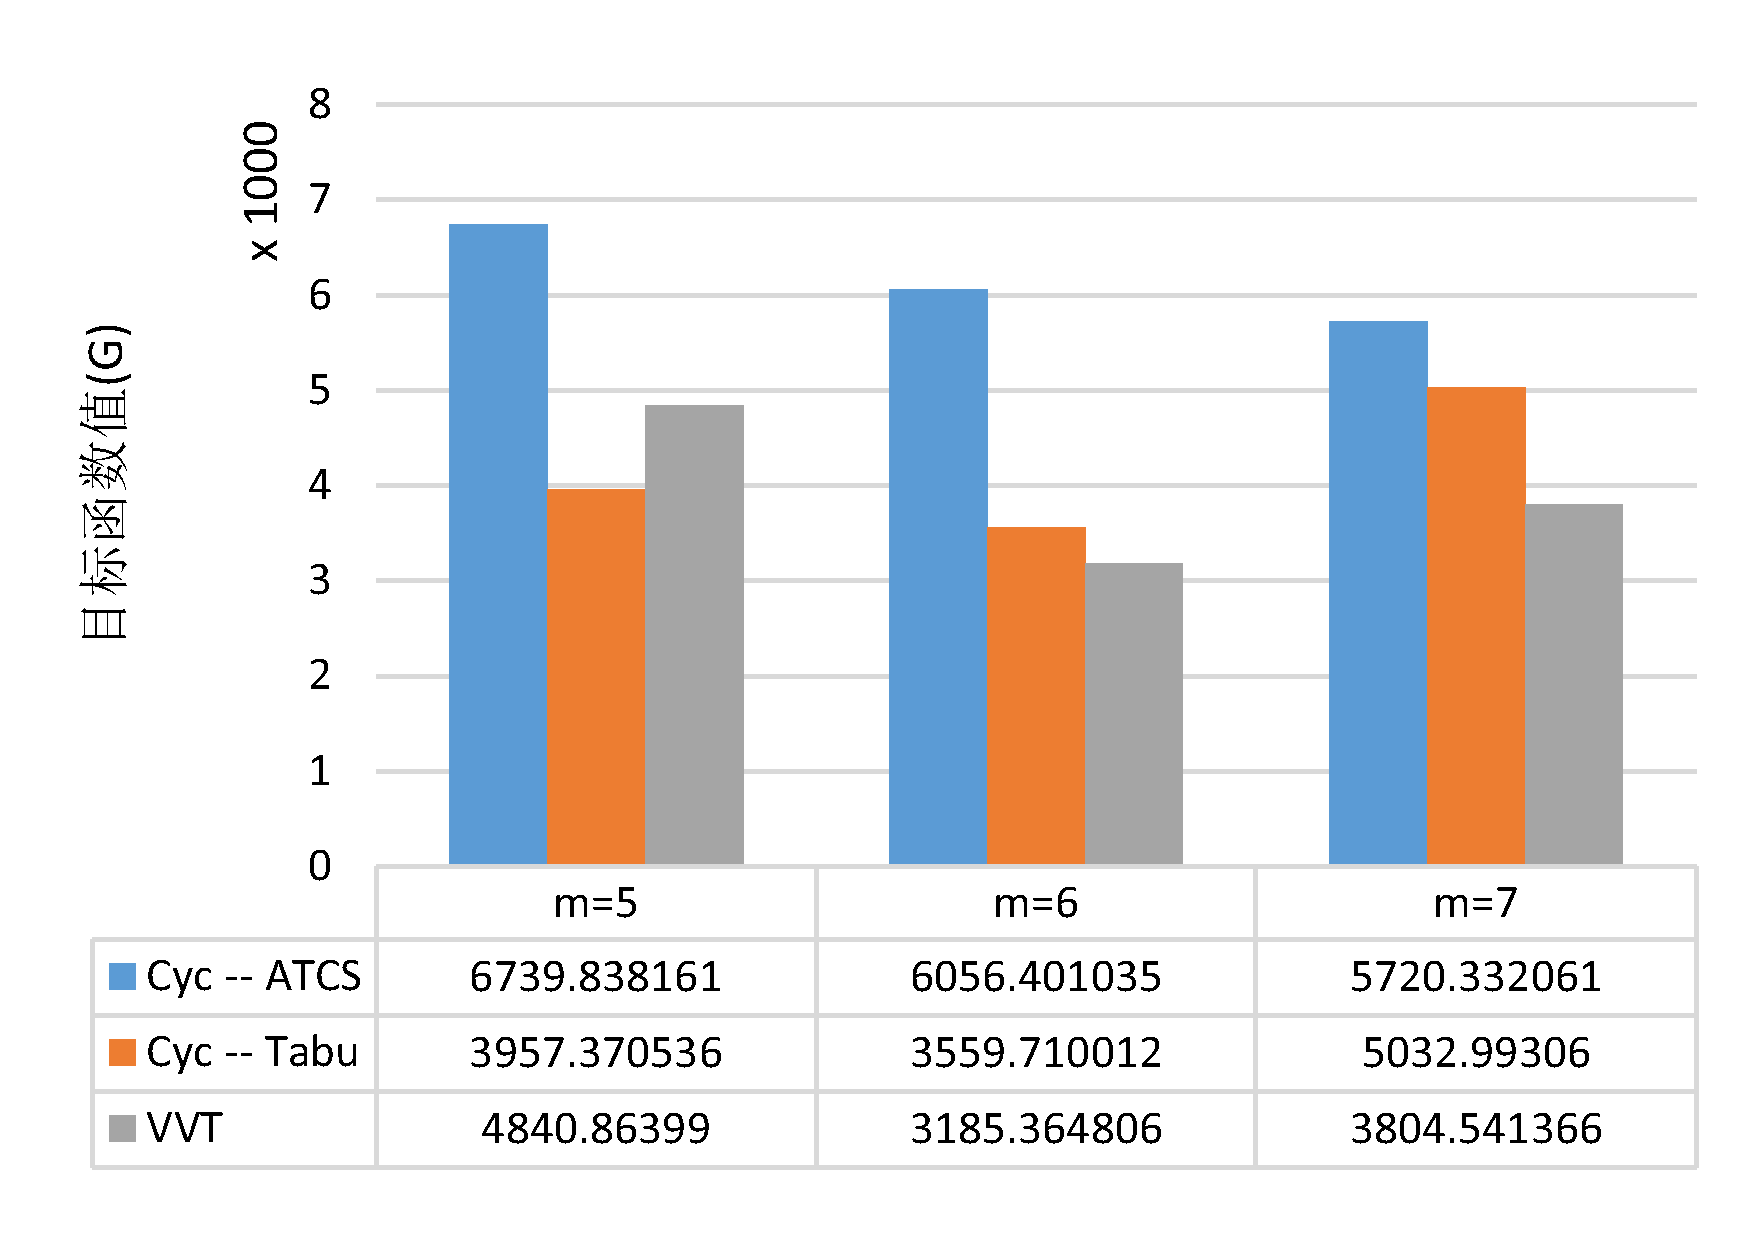
\includegraphics[height = 6cm, angle = -90]{continue_05_20}}
\subfloat[$n = 30$]{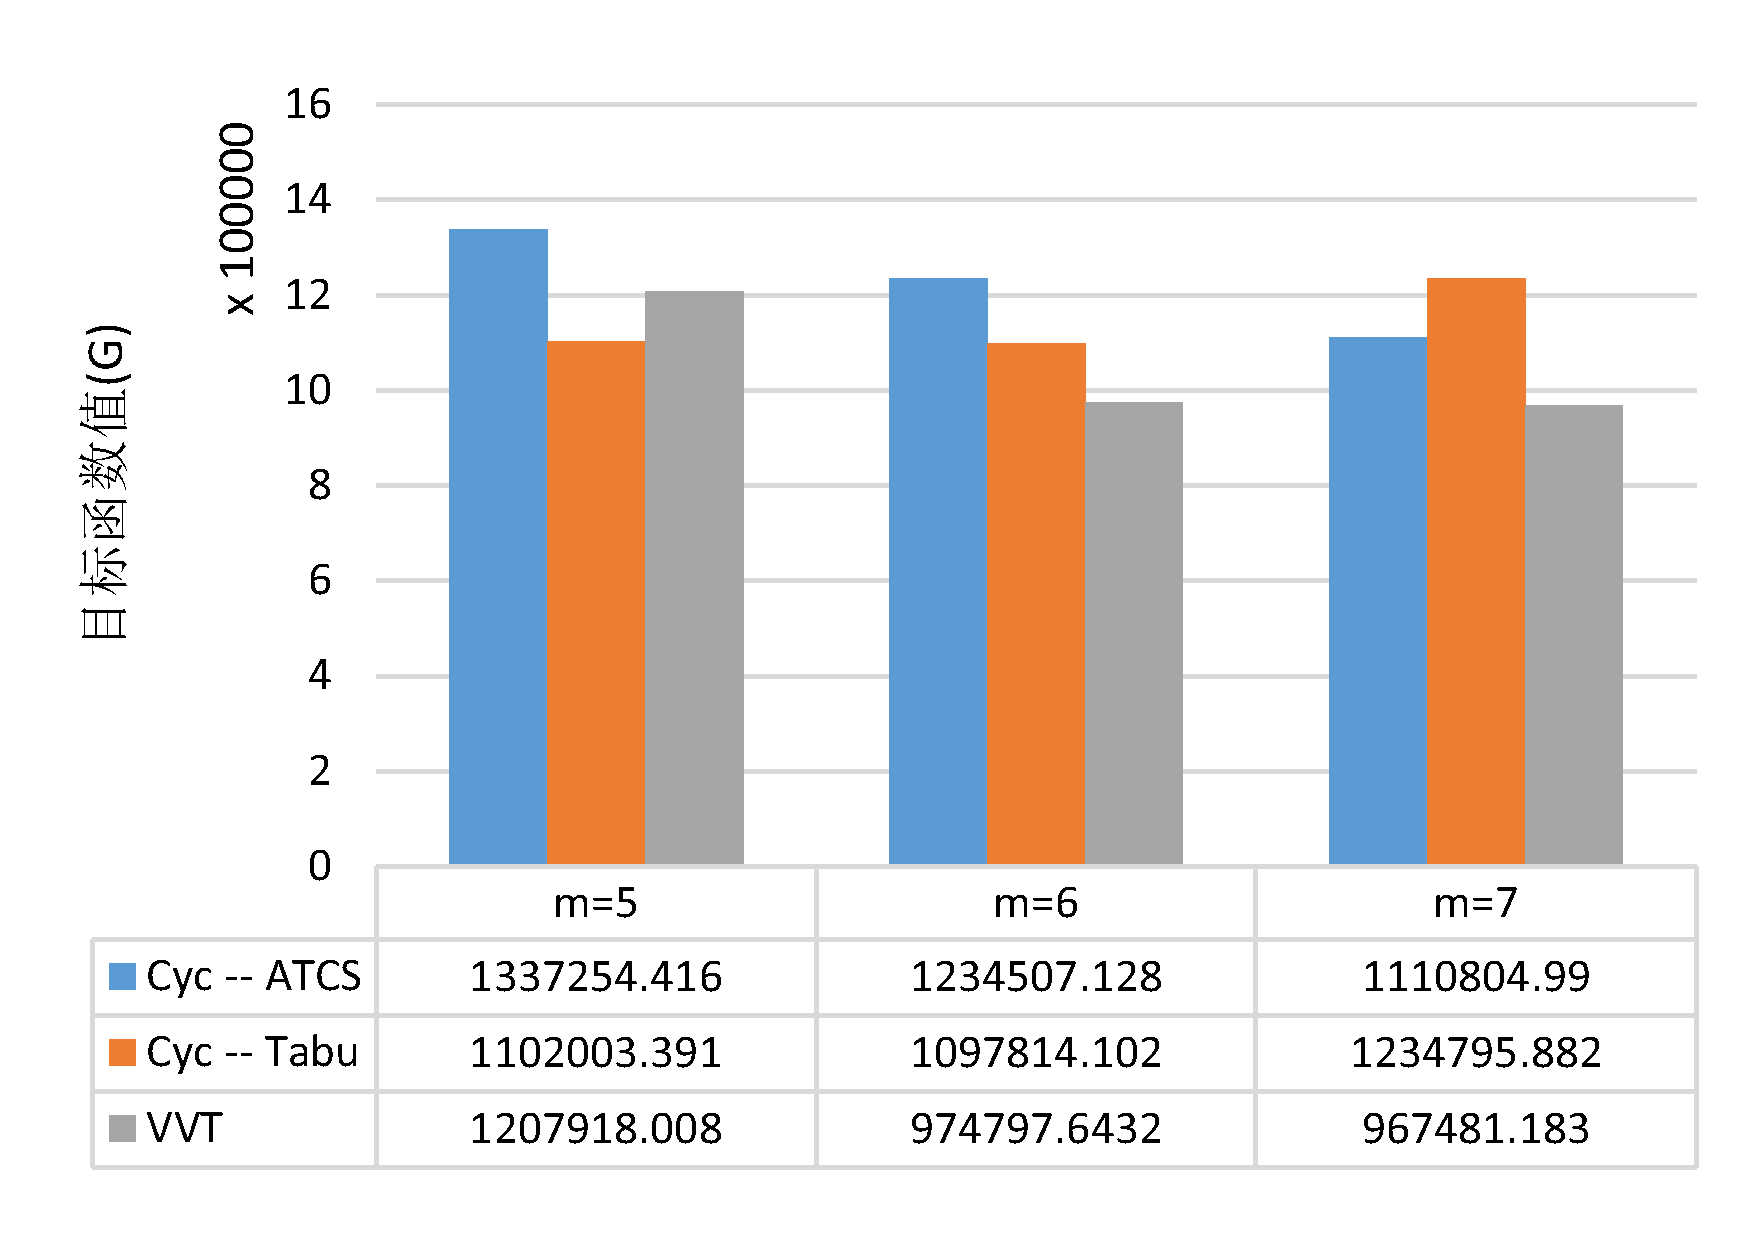
\includegraphics[height = 6cm, angle = -90]{continue_05_300}}
\subfloat[$n = 50$]{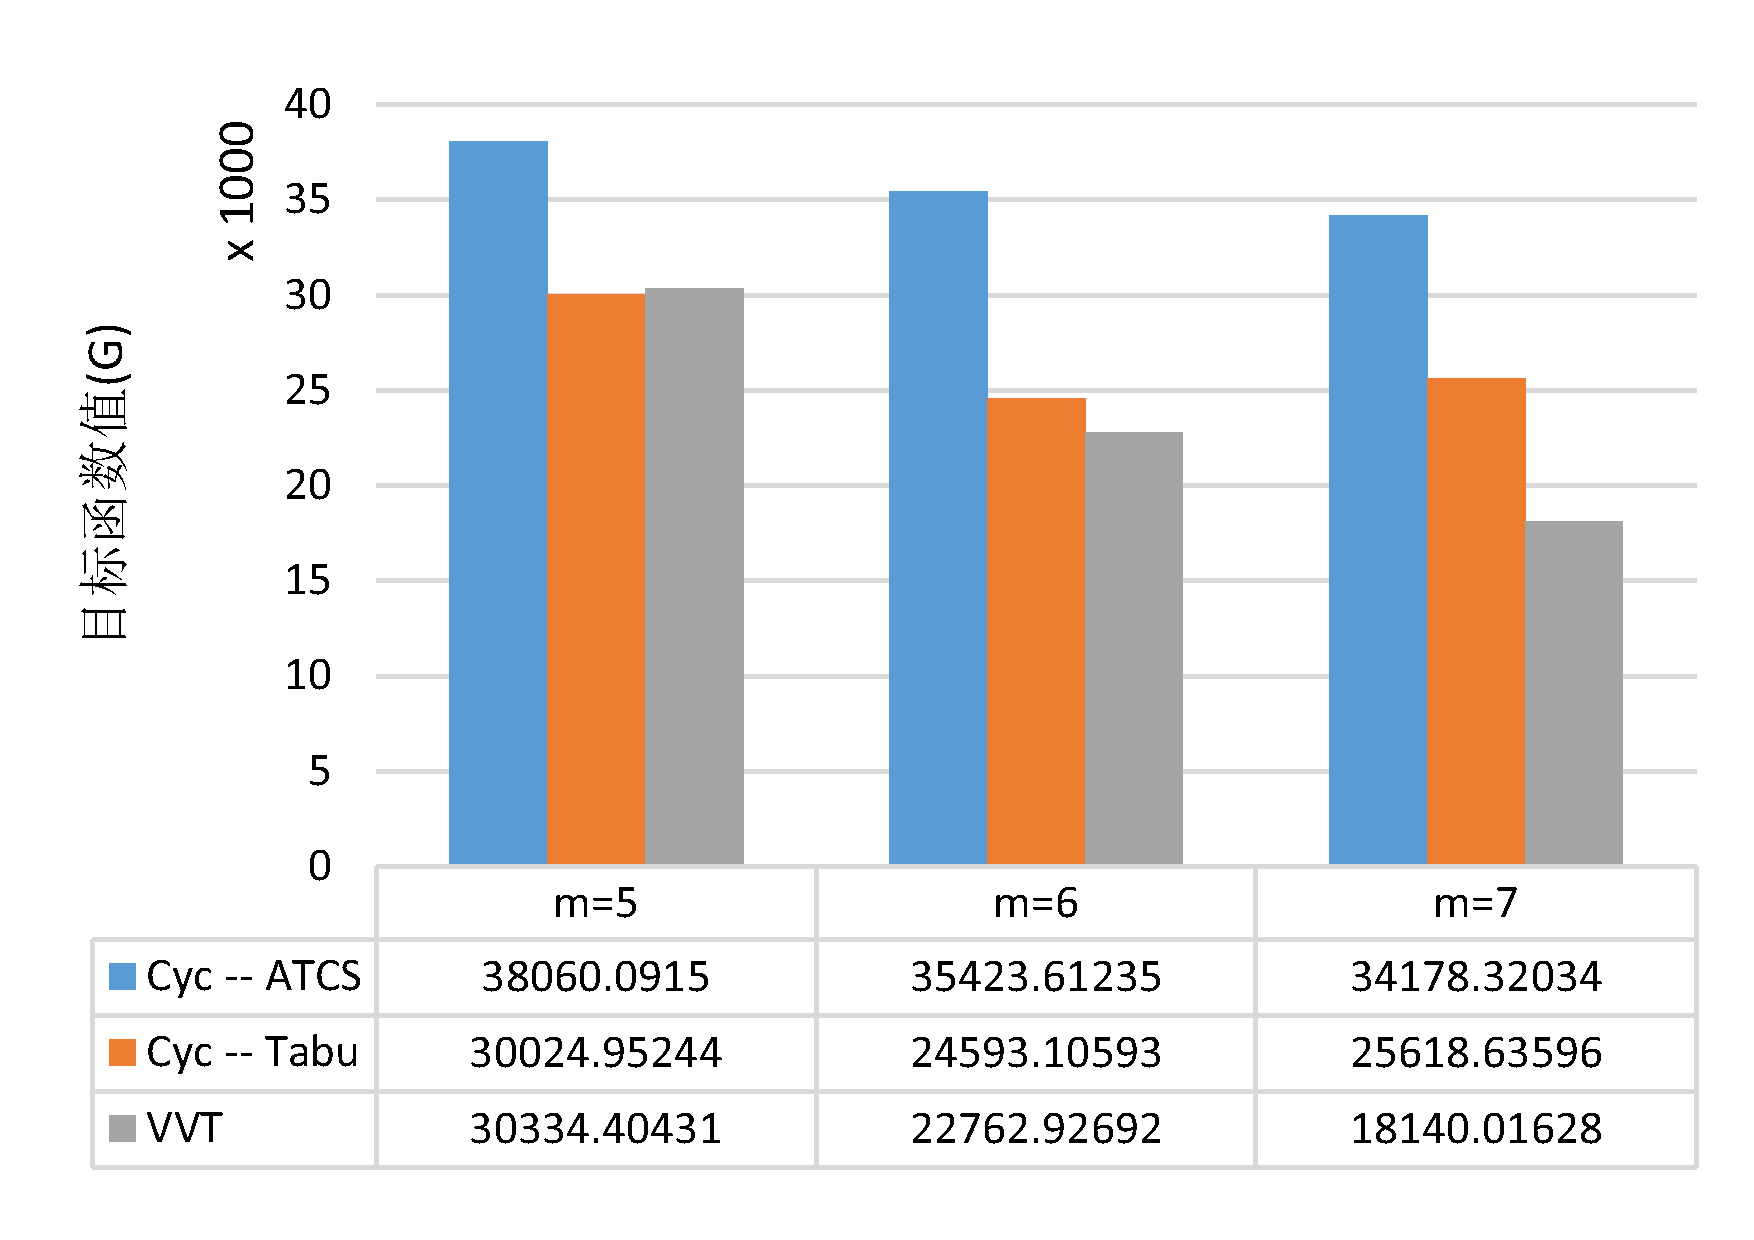
\includegraphics[height = 6cm, angle = -90]{continue_05_50}}
\subfloat[$n = 70$]{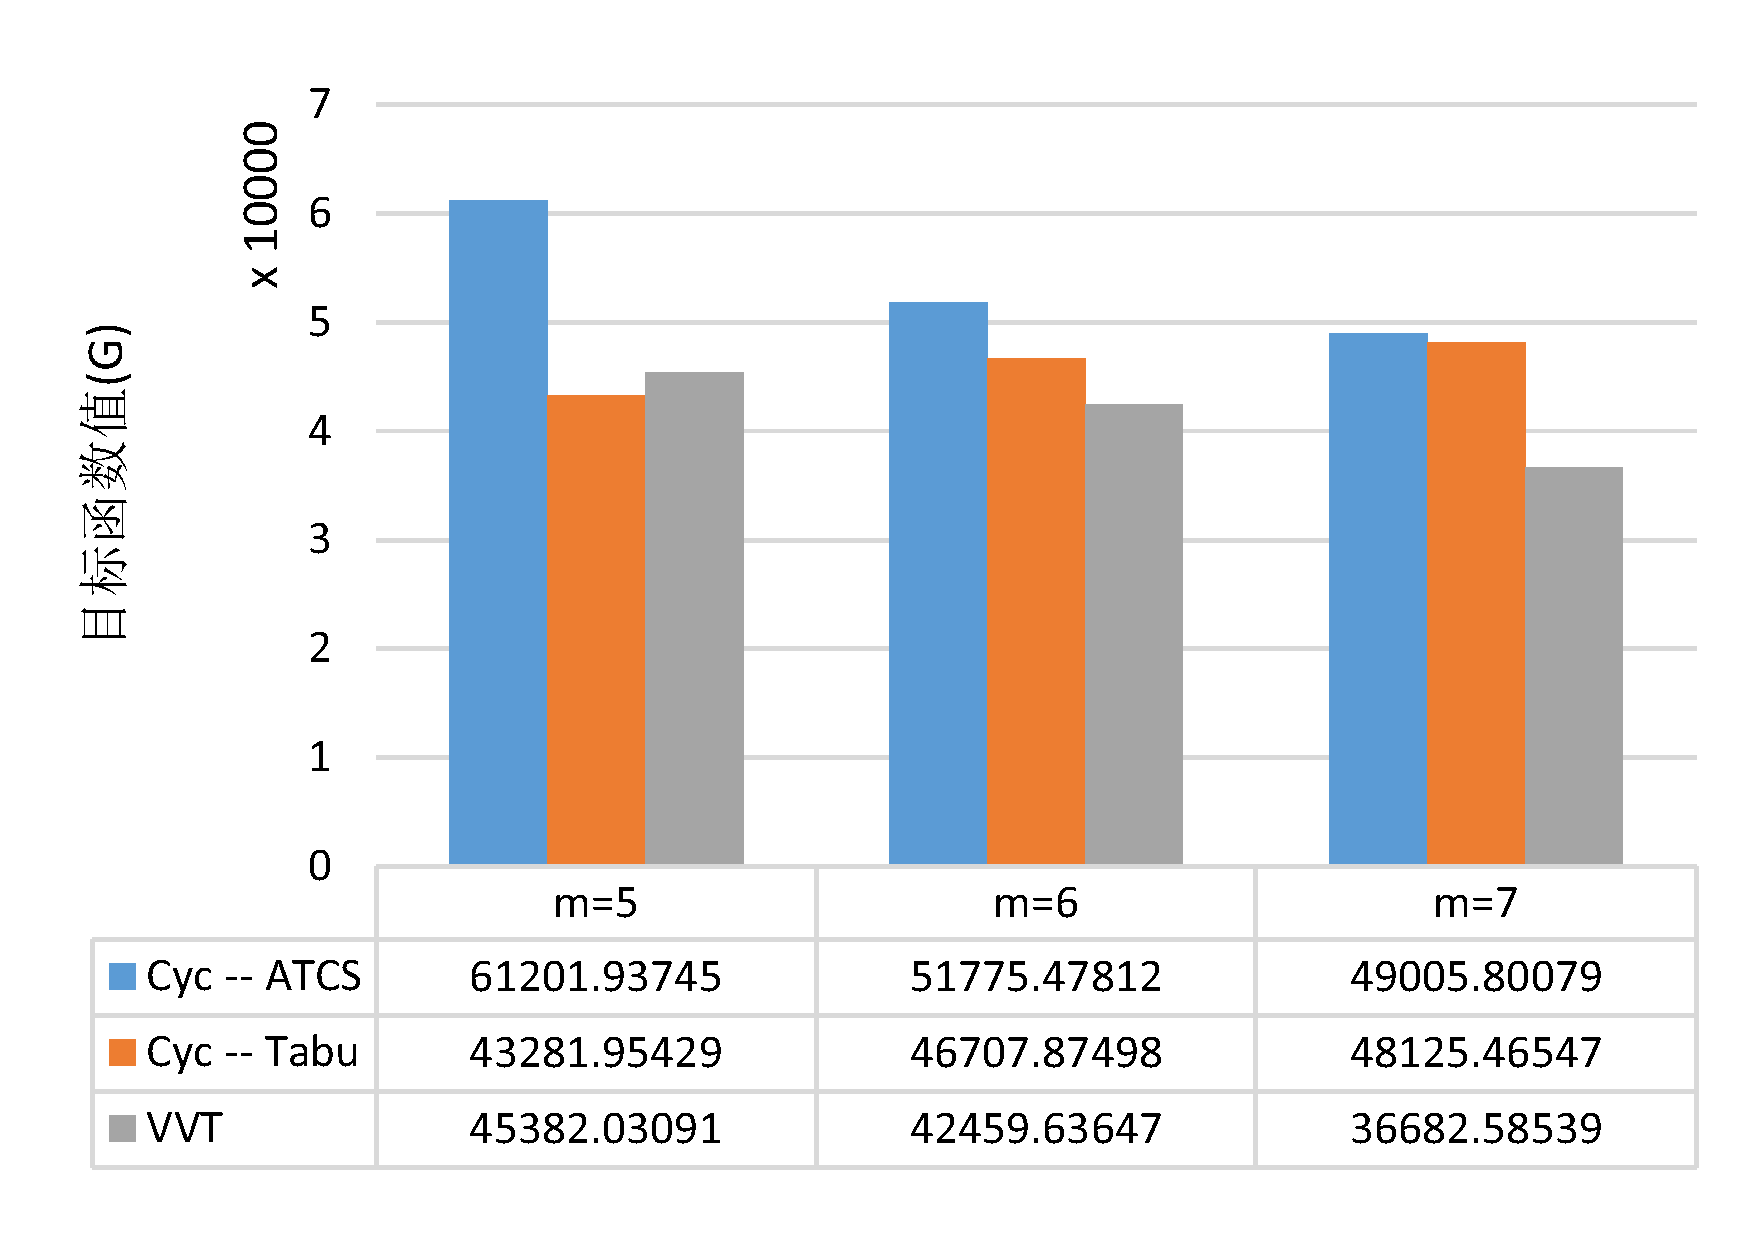
\includegraphics[height = 6cm, angle = -90]{continue_05_70}}\\
\subfloat[$n = 100$]{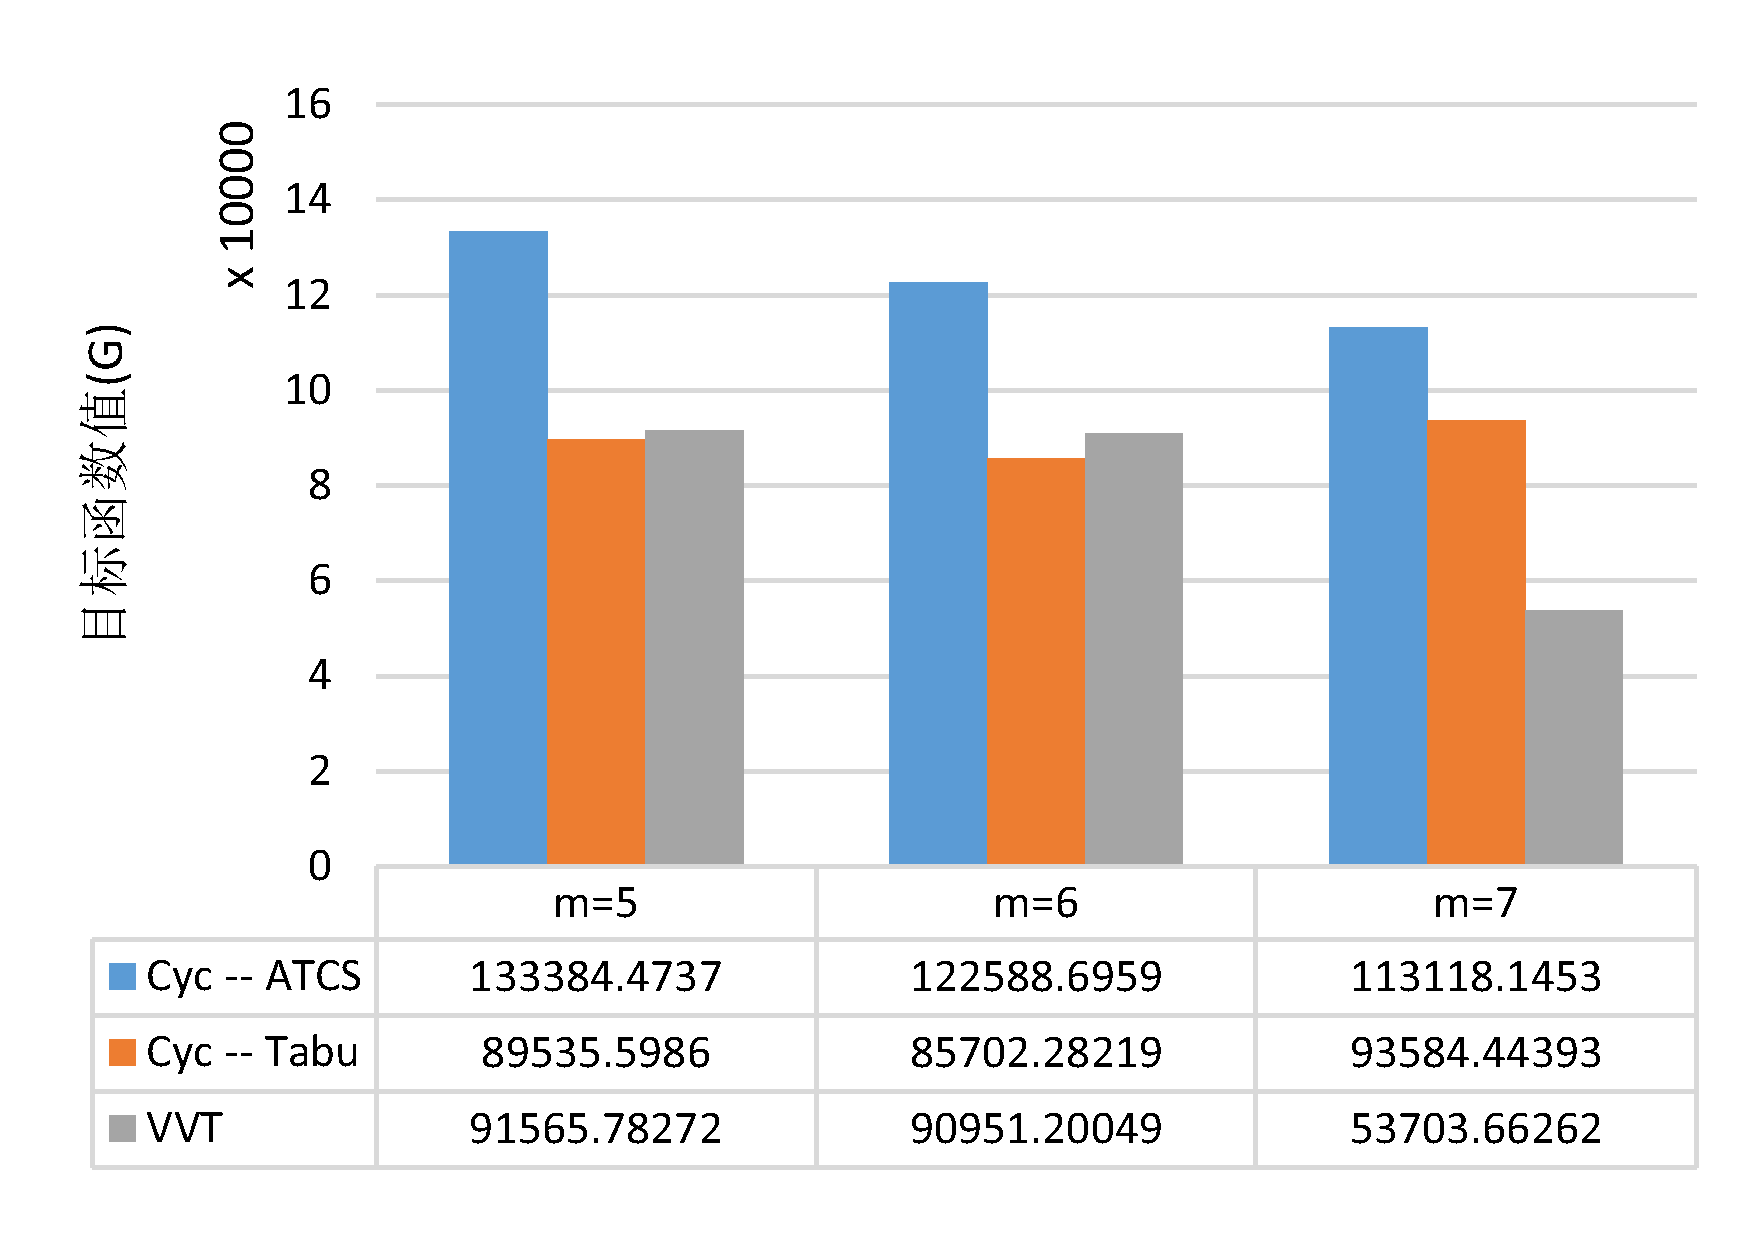
\includegraphics[height = 6cm, angle = -90]{continue_05_100}}
\subfloat[$n = 150$]{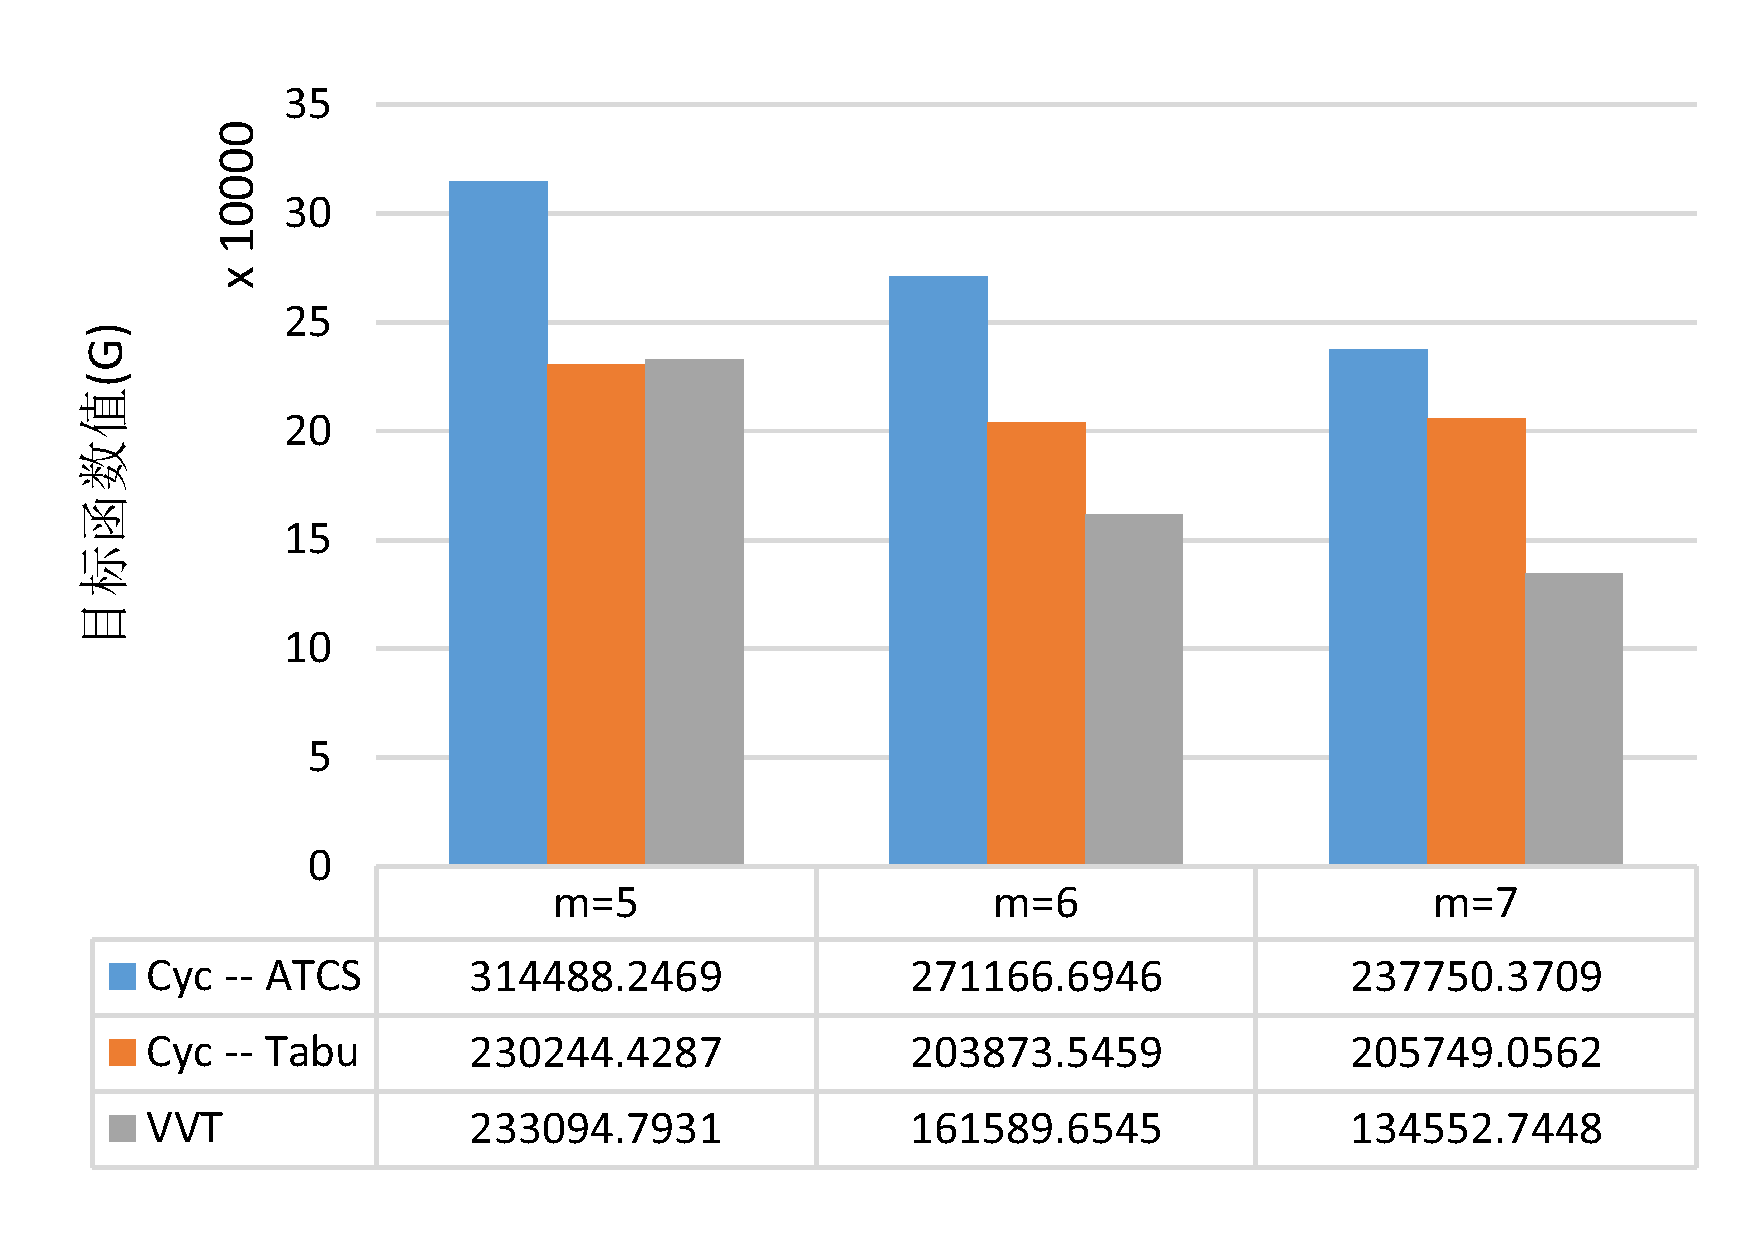
\includegraphics[height = 6cm, angle = -90]{continue_05_150}}
\subfloat[$n = 200$]{\includegraphics[height = 6cm, angle = -90]{continue_05_200}}
\subfloat[$n = 300$]{\includegraphics[height = 6cm, angle = -90]{continue_05_300}}\\
\subfloat[$n = 500$]{\includegraphics[height = 6cm, angle = -90]{continue_05_500}}
\subfloat[$n = 750$]{\includegraphics[height = 6cm, angle = -90]{continue_05_750}}
\subfloat[$n = 1000$]{\includegraphics[height = 6cm, angle = -90]{continue_05_1000}}
\caption{\label{fig:result5}模型$2$的Cyc -- ATCS、Cyc -- Tabu、VVT 算法求解目标函数值比较$(\lambda_1 = 0.5)$}
\end{sidewaysfigure}

\begin{sidewaysfigure}
\centering
\subfloat[$n = 20$]{\includegraphics[height = 6cm, angle = -90]{continue_06_20}}
\subfloat[$n = 30$]{\includegraphics[height = 6cm, angle = -90]{continue_06_300}}
\subfloat[$n = 50$]{\includegraphics[height = 6cm, angle = -90]{continue_06_50}}
\subfloat[$n = 70$]{\includegraphics[height = 6cm, angle = -90]{continue_06_70}}\\
\subfloat[$n = 100$]{\includegraphics[height = 6cm, angle = -90]{continue_06_100}}
\subfloat[$n = 150$]{\includegraphics[height = 6cm, angle = -90]{continue_06_150}}
\subfloat[$n = 200$]{\includegraphics[height = 6cm, angle = -90]{continue_06_200}}
\subfloat[$n = 300$]{\includegraphics[height = 6cm, angle = -90]{continue_06_300}}\\
\subfloat[$n = 500$]{\includegraphics[height = 6cm, angle = -90]{continue_06_500}}
\subfloat[$n = 750$]{\includegraphics[height = 6cm, angle = -90]{continue_06_750}}
\subfloat[$n = 1000$]{\includegraphics[height = 6cm, angle = -90]{continue_06_1000}}
\caption{\label{fig:result6}模型$2$的Cyc -- ATCS、Cyc -- Tabu、VVT 算法求解目标函数值比较$(\lambda_1 = 0.6)$}
\end{sidewaysfigure}

% !Mode:: "TeX:UTF-8"
% !TEX root = ..\thesis.tex
\begin{table}[htbp]
  \centering
  \caption{Cyc – ATCS、Cyc – Tabu、VVT 算法求解模型 2 所得调度流水线均衡率($\lambda_1 = 0.4$)}
    \begin{tabular}{cccccccccc}
    \toprule
$m $& \multicolumn{3}{c}{$5$} & \multicolumn{3}{c}{$6$} & \multicolumn{3}{c}{$7$} \\
\cmidrule(lr){2-4} \cmidrule(lr){5-7}\cmidrule(lr){8-10}
   $n $&(1) & (2) & (3)   &(1) & (2) & (3)   &(1) & (2) & (3) \footnote{(1): Cyc -- ATCS, (2): Cyc -- Tabu, (3): VVT, \reft{tab:rb5}与\reft{tab:rb6}与此相同}\\
  \midrule
    $20    $&$ 79.48\% $&$ 52.82\% $&$ 95.54\% $&$ 84.27\% $&$ 60.79\% $&$ 85.35\% $&$ 80.89\% $&$ 47.44\% $&$ 83.39\%$ \\
    $30    $&$ 87.39\% $&$ 81.09\% $&$ 90.53\% $&$ 86.76\% $&$ 76.63\% $&$ 85.48\% $&$ 85.28\% $&$ 76.92\% $&$ 79.37\% $\\
    $50    $&$ 94.55\% $&$ 92.44\% $&$ 95.33\% $&$ 90.03\% $&$ 90.63\% $&$ 88.33\% $&$ 93.58\% $&$ 91.78\% $&$ 86.79\% $\\
    $70    $&$ 89.91\% $&$ 93.05\% $&$ 92.99\% $&$ 93.42\% $&$ 95.08\% $&$ 93.64\% $&$ 92.62\% $&$ 93.85\% $&$ 94.06\% $\\
    $100   $&$ 97.27\% $&$ 89.14\% $&$ 91.19\% $&$ 94.38\% $&$ 88.58\% $&$ 94.10\% $&$ 94.92\% $&$ 92.98\% $&$ 83.80\% $\\
    $150   $&$ 94.77\% $&$ 93.43\% $&$ 97.24\% $&$ 95.98\% $&$ 95.03\% $&$ 94.33\% $&$ 96.57\% $&$ 96.43\% $&$ 93.09\%$ \\
    $200   $&$ 96.44\% $&$ 98.25\% $&$ 97.86\% $&$ 97.35\% $&$ 96.95\% $&$ 94.67\% $&$ 96.72\% $&$ 96.52\% $&$ 94.18\% $\\
    $300   $&$ 98.93\% $&$ 94.26\% $&$ 96.91\% $&$ 96.39\% $&$ 92.82\% $&$ 96.09\% $&$ 97.61\% $&$ 92.57\% $&$ 97.56\% $\\
    $500   $&$ 97.42\% $&$ 97.29\% $&$ 99.25\% $&$ 98.07\% $&$ 97.76\% $&$ 98.62\% $&$ 97.70\% $&$ 97.79\% $&$ 99.26\% $\\
    $750   $&$ 98.52\% $&$ 98.33\% $&$ 99.26\% $&$ 98.10\% $&$ 97.65\% $&$ 98.82\% $&$ 96.48\% $&$ 98.50\% $&$ 98.98\% $\\
    $1000  $&$ 99.42\% $&$ 99.23\% $&$ 99.80\% $&$ 99.42\% $&$ 99.85\% $&$ 99.78\% $&$ 99.42\% $&$ 99.51\% $&$ 99.44\% $\\
    \bottomrule
    \end{tabular}
  \label{tab:rb4}
\end{table}
% !Mode:: "TeX:UTF-8"
% !TEX root = ..\thesis.tex
\begin{table}[htbp]
  \centering
  \caption{Cyc – ATCS、Cyc – Tabu、VVT 算法求解模型 2 所得调度流水线均衡率($\lambda_1 = 0.5$)}
    \begin{tabular}{cccccccccc}
    \toprule
$m $& \multicolumn{3}{c}{$5$} & \multicolumn{3}{c}{$6$} & \multicolumn{3}{c}{$7$} \\
    \cmidrule(lr){2-4} \cmidrule(lr){5-7}\cmidrule(lr){8-10}
$n $& (1)& (2) & (3)   & (1)& (2) & (3)   & (1)& (2) & (3) \\
      \midrule
    $20    $&$ 79.48\% $&$ 54.65\% $&$ 93.47\% $&$ 79.86\% $&$ 60.00\% $&$ 86.38\% $&$ 87.38\% $&$ 74.07\% $&$ 80.95\% $\\
    $30    $&$ 87.39\% $&$ 79.09\% $&$ 93.58\% $&$ 86.76\% $&$ 80.45\% $&$ 80.39\% $&$ 85.28\% $&$ 71.85\% $&$ 83.89\% $\\
    $50    $&$ 94.31\% $&$ 88.52\% $&$ 94.49\% $&$ 90.03\% $&$ 87.09\% $&$ 89.90\% $&$ 94.44\% $&$ 92.35\% $&$ 89.13\% $\\
    $70    $&$ 89.91\% $&$ 87.56\% $&$ 93.53\% $&$ 93.42\% $&$ 90.43\% $&$ 91.80\% $&$ 89.89\% $&$ 86.93\% $&$ 93.16\% $\\
    $100   $&$ 91.81\% $&$ 88.89\% $&$ 92.57\% $&$ 94.89\% $&$ 90.97\% $&$ 91.27\% $&$ 94.77\% $&$ 93.79\% $&$ 90.01\% $\\
    $150   $&$ 94.77\% $&$ 94.48\% $&$ 96.72\% $&$ 95.98\% $&$ 94.76\% $&$ 93.50\% $&$ 96.57\% $&$ 93.61\% $&$ 94.22\% $\\
    $200   $&$ 96.44\% $&$ 97.77\% $&$ 96.29\% $&$ 97.35\% $&$ 98.75\% $&$ 96.03\% $&$ 96.36\% $&$ 98.24\% $&$ 96.52\% $\\
    $300   $&$ 98.93\% $&$ 93.38\% $&$ 97.50\% $&$ 96.39\% $&$ 93.74\% $&$ 97.71\% $&$ 97.66\% $&$ 94.16\% $&$ 98.01\% $\\
    $500   $&$ 97.64\% $&$ 97.15\% $&$ 99.08\% $&$ 98.07\% $&$ 96.81\% $&$ 98.74\% $&$ 97.70\% $&$ 97.16\% $&$ 98.62\% $\\
    $750   $&$ 99.38\% $&$ 98.85\% $&$ 99.40\% $&$ 98.23\% $&$ 98.56\% $&$ 99.36\% $&$ 96.48\% $&$ 98.53\% $&$ 98.56\% $\\
    $1000  $&$ 99.88\% $&$ 99.36\% $&$ 99.80\% $&$ 99.88\% $&$ 99.69\% $&$ 99.68\% $&$ 99.88\% $&$ 99.31\% $&$ 99.71\% $\\
    \bottomrule
    \end{tabular}
  \label{tab:rb5}
\end{table}
% !Mode:: "TeX:UTF-8"
% !TEX root = ..\thesis.tex
\begin{table}[htbp]
  \centering
  \caption{Cyc – ATCS、Cyc – Tabu、VVT 算法求解模型 2 所得调度流水线均衡率($\lambda_1 = 0.6$)}
    \begin{tabular}{cccccccccc}
    \toprule
$m $& \multicolumn{3}{c}{$5$} & \multicolumn{3}{c}{$6$} & \multicolumn{3}{c}{$7$} \\
    \cmidrule(lr){2-4} \cmidrule(lr){5-7}\cmidrule(lr){8-10}
$n $& (1)& (2) & (3)   & (1)& (2) & (3)   & (1) & (2) & (3) \\
        \midrule
    $20    $&$ 84.80\% $&$ 54.88\% $&$ 82.53\% $&$ 79.86\% $&$ 57.16\% $&$ 84.85\% $&$ 87.38\% $&$ 59.22\% $&$ 78.30\% $\\
    $30    $&$ 92.27\% $&$ 91.21\% $&$ 82.63\% $&$ 86.76\% $&$ 88.40\% $&$ 75.45\% $&$ 87.17\% $&$ 70.37\% $&$ 77.28\% $\\
    $50    $&$ 94.31\% $&$ 92.23\% $&$ 89.35\% $&$ 90.03\% $&$ 87.73\% $&$ 91.42\% $&$ 88.18\% $&$ 85.47\% $&$ 87.31\% $\\
    $70    $&$ 89.91\% $&$ 88.36\% $&$ 96.05\% $&$ 93.42\% $&$ 92.21\% $&$ 94.86\% $&$ 92.84\% $&$ 89.04\% $&$ 93.19\% $\\
    $100   $&$ 93.60\% $&$ 91.69\% $&$ 98.10\% $&$ 94.89\% $&$ 92.06\% $&$ 91.83\% $&$ 94.77\% $&$ 88.66\% $&$ 91.72\% $\\
    $150   $&$ 96.08\% $&$ 94.90\% $&$ 93.63\% $&$ 95.98\% $&$ 95.36\% $&$ 94.65\% $&$ 96.57\% $&$ 91.93\% $&$ 92.51\% $\\
    $200   $&$ 96.44\% $&$ 96.74\% $&$ 98.71\% $&$ 97.46\% $&$ 97.70\% $&$ 95.17\% $&$ 97.59\% $&$ 98.36\% $&$ 95.38\% $\\
    $300   $&$ 98.80\% $&$ 94.03\% $&$ 95.23\% $&$ 96.39\% $&$ 94.75\% $&$ 96.43\% $&$ 96.54\% $&$ 94.83\% $&$ 97.27\% $\\
    $500   $&$ 96.41\% $&$ 96.01\% $&$ 99.14\% $&$ 98.20\% $&$ 97.01\% $&$ 99.44\% $&$ 96.56\% $&$ 98.08\% $&$ 98.57\% $\\
    $750   $&$ 99.38\% $&$ 97.77\% $&$ 99.10\% $&$ 98.23\% $&$ 97.94\% $&$ 99.31\% $&$ 96.10\% $&$ 99.27\% $&$ 99.26\% $\\
    $1000  $&$ 99.39\% $&$ 99.49\% $&$ 99.67\% $&$ 99.39\% $&$ 99.67\% $&$ 99.72\% $&$ 99.39\% $&$ 99.42\% $&$ 99.49\% $\\
    \bottomrule
    \end{tabular}
  \label{tab:rb6}
\end{table}
\begin{sidewaysfigure}
\centering
\subfloat[$n = 20$]{\includegraphics[height = 6cm, angle = -90]{Rb_04_20}}
\subfloat[$n = 30$]{\includegraphics[height = 6cm, angle = -90]{Rb_04_300}}
\subfloat[$n = 50$]{\includegraphics[height = 6cm, angle = -90]{Rb_04_50}}
\subfloat[$n = 70$]{\includegraphics[height = 6cm, angle = -90]{Rb_04_70}}\\
\subfloat[$n = 100$]{\includegraphics[height = 6cm, angle = -90]{Rb_04_100}}
\subfloat[$n = 150$]{\includegraphics[height = 6cm, angle = -90]{Rb_04_150}}
\subfloat[$n = 200$]{\includegraphics[height = 6cm, angle = -90]{Rb_04_200}}
\subfloat[$n = 300$]{\includegraphics[height = 6cm, angle = -90]{Rb_04_300}}\\
\subfloat[$n = 500$]{\includegraphics[height = 6cm, angle = -90]{Rb_04_500}}
\subfloat[$n = 750$]{\includegraphics[height = 6cm, angle = -90]{Rb_04_750}}
\subfloat[$n = 1000$]{\includegraphics[height = 6cm, angle = -90]{Rb_04_1000}}
\caption{\label{fig:result7}模型$2$的Cyc -- ATCS、Cyc -- Tabu、VVT 算法求解流水线均衡率比较$(\lambda_1 = 0.4)$}
\end{sidewaysfigure}

\begin{sidewaysfigure}
\centering
\subfloat[$n = 20$]{\includegraphics[height = 6cm, angle = -90]{Rb_05_20}}
\subfloat[$n = 30$]{\includegraphics[height = 6cm, angle = -90]{Rb_05_300}}
\subfloat[$n = 50$]{\includegraphics[height = 6cm, angle = -90]{Rb_05_50}}
\subfloat[$n = 70$]{\includegraphics[height = 6cm, angle = -90]{Rb_05_70}}\\
\subfloat[$n = 100$]{\includegraphics[height = 6cm, angle = -90]{Rb_05_100}}
\subfloat[$n = 150$]{\includegraphics[height = 6cm, angle = -90]{Rb_05_150}}
\subfloat[$n = 200$]{\includegraphics[height = 6cm, angle = -90]{Rb_05_200}}
\subfloat[$n = 300$]{\includegraphics[height = 6cm, angle = -90]{Rb_05_300}}\\
\subfloat[$n = 500$]{\includegraphics[height = 6cm, angle = -90]{Rb_05_500}}
\subfloat[$n = 750$]{\includegraphics[height = 6cm, angle = -90]{Rb_05_750}}
\subfloat[$n = 1000$]{\includegraphics[height = 6cm, angle = -90]{Rb_05_1000}}
\caption{\label{fig:result8}模型$2$的Cyc -- ATCS、Cyc -- Tabu、VVT 算法求解流水线均衡率比较$(\lambda_1 = 0.5)$}
\end{sidewaysfigure}

\begin{sidewaysfigure}
\centering
\subfloat[$n = 20$]{\includegraphics[height = 6cm, angle = -90]{Rb_06_20}}
\subfloat[$n = 30$]{\includegraphics[height = 6cm, angle = -90]{Rb_06_300}}
\subfloat[$n = 50$]{\includegraphics[height = 6cm, angle = -90]{Rb_06_50}}
\subfloat[$n = 70$]{\includegraphics[height = 6cm, angle = -90]{Rb_06_70}}\\
\subfloat[$n = 100$]{\includegraphics[height = 6cm, angle = -90]{Rb_06_100}}
\subfloat[$n = 150$]{\includegraphics[height = 6cm, angle = -90]{Rb_06_150}}
\subfloat[$n = 200$]{\includegraphics[height = 6cm, angle = -90]{Rb_06_200}}
\subfloat[$n = 300$]{\includegraphics[height = 6cm, angle = -90]{Rb_06_300}}\\
\subfloat[$n = 500$]{\includegraphics[height = 6cm, angle = -90]{Rb_06_500}}
\subfloat[$n = 750$]{\includegraphics[height = 6cm, angle = -90]{Rb_06_750}}
\subfloat[$n = 1000$]{\includegraphics[height = 6cm, angle = -90]{Rb_06_1000}}
\caption{\label{fig:result9}模型$2$的Cyc -- ATCS、Cyc -- Tabu、VVT 算法求解流水线均衡率比较$(\lambda_1 = 0.6)$}
\end{sidewaysfigure}



